\documentclass[twoside]{book}

% Packages required by doxygen
\usepackage{fixltx2e}
\usepackage{calc}
\usepackage{doxygen}
\usepackage[export]{adjustbox} % also loads graphicx
\usepackage{graphicx}
\usepackage[utf8]{inputenc}
\usepackage{makeidx}
\usepackage{multicol}
\usepackage{multirow}
\PassOptionsToPackage{warn}{textcomp}
\usepackage{textcomp}
\usepackage[nointegrals]{wasysym}
\usepackage[table]{xcolor}

% Font selection
\usepackage[T1]{fontenc}
\usepackage[scaled=.90]{helvet}
\usepackage{courier}
\usepackage{amssymb}
\usepackage{sectsty}
\renewcommand{\familydefault}{\sfdefault}
\allsectionsfont{%
  \fontseries{bc}\selectfont%
  \color{darkgray}%
}
\renewcommand{\DoxyLabelFont}{%
  \fontseries{bc}\selectfont%
  \color{darkgray}%
}
\newcommand{\+}{\discretionary{\mbox{\scriptsize$\hookleftarrow$}}{}{}}

% Page & text layout
\usepackage{geometry}
\geometry{%
  a4paper,%
  top=2.5cm,%
  bottom=2.5cm,%
  left=2.5cm,%
  right=2.5cm%
}
\tolerance=750
\hfuzz=15pt
\hbadness=750
\setlength{\emergencystretch}{15pt}
\setlength{\parindent}{0cm}
\setlength{\parskip}{3ex plus 2ex minus 2ex}
\makeatletter
\renewcommand{\paragraph}{%
  \@startsection{paragraph}{4}{0ex}{-1.0ex}{1.0ex}{%
    \normalfont\normalsize\bfseries\SS@parafont%
  }%
}
\renewcommand{\subparagraph}{%
  \@startsection{subparagraph}{5}{0ex}{-1.0ex}{1.0ex}{%
    \normalfont\normalsize\bfseries\SS@subparafont%
  }%
}
\makeatother

% Headers & footers
\usepackage{fancyhdr}
\pagestyle{fancyplain}
\fancyhead[LE]{\fancyplain{}{\bfseries\thepage}}
\fancyhead[CE]{\fancyplain{}{}}
\fancyhead[RE]{\fancyplain{}{\bfseries\leftmark}}
\fancyhead[LO]{\fancyplain{}{\bfseries\rightmark}}
\fancyhead[CO]{\fancyplain{}{}}
\fancyhead[RO]{\fancyplain{}{\bfseries\thepage}}
\fancyfoot[LE]{\fancyplain{}{}}
\fancyfoot[CE]{\fancyplain{}{}}
\fancyfoot[RE]{\fancyplain{}{\bfseries\scriptsize Generated by Doxygen }}
\fancyfoot[LO]{\fancyplain{}{\bfseries\scriptsize Generated by Doxygen }}
\fancyfoot[CO]{\fancyplain{}{}}
\fancyfoot[RO]{\fancyplain{}{}}
\renewcommand{\footrulewidth}{0.4pt}
\renewcommand{\chaptermark}[1]{%
  \markboth{#1}{}%
}
\renewcommand{\sectionmark}[1]{%
  \markright{\thesection\ #1}%
}

% Indices & bibliography
\usepackage{natbib}
\usepackage[titles]{tocloft}
\setcounter{tocdepth}{3}
\setcounter{secnumdepth}{5}
\makeindex

% Hyperlinks (required, but should be loaded last)
\usepackage{ifpdf}
\ifpdf
  \usepackage[pdftex,pagebackref=true]{hyperref}
\else
  \usepackage[ps2pdf,pagebackref=true]{hyperref}
\fi
\hypersetup{%
  colorlinks=true,%
  linkcolor=blue,%
  citecolor=blue,%
  unicode%
}

% Custom commands
\newcommand{\clearemptydoublepage}{%
  \newpage{\pagestyle{empty}\cleardoublepage}%
}

\usepackage{caption}
\captionsetup{labelsep=space,justification=centering,font={bf},singlelinecheck=off,skip=4pt,position=top}

%===== C O N T E N T S =====

\begin{document}

% Titlepage & ToC
\hypersetup{pageanchor=false,
             bookmarksnumbered=true,
             pdfencoding=unicode
            }
\pagenumbering{alph}
\begin{titlepage}
\vspace*{7cm}
\begin{center}%
{\Large My Project }\\
\vspace*{1cm}
{\large Generated by Doxygen 1.8.14}\\
\end{center}
\end{titlepage}
\clearemptydoublepage
\pagenumbering{roman}
\tableofcontents
\clearemptydoublepage
\pagenumbering{arabic}
\hypersetup{pageanchor=true}

%--- Begin generated contents ---
\chapter{Hierarchical Index}
\section{Class Hierarchy}
This inheritance list is sorted roughly, but not completely, alphabetically\+:\begin{DoxyCompactList}
\item \contentsline{section}{C\+Aquarium}{\pageref{class_c_aquarium}}{}
\item C\+Dialog\+Ex\begin{DoxyCompactList}
\item \contentsline{section}{C\+About\+Dlg}{\pageref{class_c_about_dlg}}{}
\end{DoxyCompactList}
\item C\+Frame\+Wnd\begin{DoxyCompactList}
\item \contentsline{section}{C\+Main\+Frame}{\pageref{class_c_main_frame}}{}
\end{DoxyCompactList}
\item \contentsline{section}{C\+Item}{\pageref{class_c_item}}{}
\begin{DoxyCompactList}
\item \contentsline{section}{C\+Fish\+Beta}{\pageref{class_c_fish_beta}}{}
\end{DoxyCompactList}
\item C\+Win\+App\begin{DoxyCompactList}
\item \contentsline{section}{C\+Step2\+App}{\pageref{class_c_step2_app}}{}
\end{DoxyCompactList}
\item C\+Wnd\begin{DoxyCompactList}
\item \contentsline{section}{C\+Child\+View}{\pageref{class_c_child_view}}{}
\end{DoxyCompactList}
\end{DoxyCompactList}

\chapter{Class Index}
\section{Class List}
Here are the classes, structs, unions and interfaces with brief descriptions\+:\begin{DoxyCompactList}
\item\contentsline{section}{\mbox{\hyperlink{class_c_about_dlg}{C\+About\+Dlg}} }{\pageref{class_c_about_dlg}}{}
\item\contentsline{section}{\mbox{\hyperlink{class_c_aquarium}{C\+Aquarium}} }{\pageref{class_c_aquarium}}{}
\item\contentsline{section}{\mbox{\hyperlink{class_c_child_view}{C\+Child\+View}} }{\pageref{class_c_child_view}}{}
\item\contentsline{section}{\mbox{\hyperlink{class_c_decor_castle}{C\+Decor\+Castle}} }{\pageref{class_c_decor_castle}}{}
\item\contentsline{section}{\mbox{\hyperlink{class_c_fish}{C\+Fish}} }{\pageref{class_c_fish}}{}
\item\contentsline{section}{\mbox{\hyperlink{class_c_fish_beta}{C\+Fish\+Beta}} }{\pageref{class_c_fish_beta}}{}
\item\contentsline{section}{\mbox{\hyperlink{class_c_fish_dory}{C\+Fish\+Dory}} }{\pageref{class_c_fish_dory}}{}
\item\contentsline{section}{\mbox{\hyperlink{class_c_fish_karp}{C\+Fish\+Karp}} }{\pageref{class_c_fish_karp}}{}
\item\contentsline{section}{\mbox{\hyperlink{class_c_fish_nemo}{C\+Fish\+Nemo}} }{\pageref{class_c_fish_nemo}}{}
\item\contentsline{section}{\mbox{\hyperlink{classxmlnode_1_1_c_xml_node_1_1_children}{xmlnode\+::\+C\+Xml\+Node\+::\+Children}} \\*Representation of children to support iteration }{\pageref{classxmlnode_1_1_c_xml_node_1_1_children}}{}
\item\contentsline{section}{\mbox{\hyperlink{class_c_item}{C\+Item}} }{\pageref{class_c_item}}{}
\item\contentsline{section}{\mbox{\hyperlink{class_c_main_frame}{C\+Main\+Frame}} }{\pageref{class_c_main_frame}}{}
\item\contentsline{section}{\mbox{\hyperlink{class_c_step2_app}{C\+Step2\+App}} }{\pageref{class_c_step2_app}}{}
\item\contentsline{section}{\mbox{\hyperlink{classxmlnode_1_1_c_xml_node}{xmlnode\+::\+C\+Xml\+Node}} \\*A wrapper for msxml nodes }{\pageref{classxmlnode_1_1_c_xml_node}}{}
\item\contentsline{section}{\mbox{\hyperlink{classxmlnode_1_1_c_xml_node_1_1_exception}{xmlnode\+::\+C\+Xml\+Node\+::\+Exception}} \\*Exceptions for \mbox{\hyperlink{classxmlnode_1_1_c_xml_node}{C\+Xml\+Node}} }{\pageref{classxmlnode_1_1_c_xml_node_1_1_exception}}{}
\item\contentsline{section}{\mbox{\hyperlink{classxmlnode_1_1_c_xml_node_1_1_iterator}{xmlnode\+::\+C\+Xml\+Node\+::\+Iterator}} \\*Support for iterating over the children of a node }{\pageref{classxmlnode_1_1_c_xml_node_1_1_iterator}}{}
\end{DoxyCompactList}

\chapter{File Index}
\section{File List}
Here is a list of all documented files with brief descriptions\+:\begin{DoxyCompactList}
\item\contentsline{section}{\mbox{\hyperlink{_aquarium_8cpp}{Aquarium.\+cpp}} }{\pageref{_aquarium_8cpp}}{}
\item\contentsline{section}{\mbox{\hyperlink{_aquarium_8h}{Aquarium.\+h}} }{\pageref{_aquarium_8h}}{}
\item\contentsline{section}{\mbox{\hyperlink{_child_view_8cpp}{Child\+View.\+cpp}} }{\pageref{_child_view_8cpp}}{}
\item\contentsline{section}{\mbox{\hyperlink{_child_view_8h}{Child\+View.\+h}} }{\pageref{_child_view_8h}}{}
\item\contentsline{section}{\mbox{\hyperlink{_fish_beta_8cpp}{Fish\+Beta.\+cpp}} }{\pageref{_fish_beta_8cpp}}{}
\item\contentsline{section}{\mbox{\hyperlink{_fish_beta_8h}{Fish\+Beta.\+h}} }{\pageref{_fish_beta_8h}}{}
\item\contentsline{section}{\mbox{\hyperlink{_item_8cpp}{Item.\+cpp}} }{\pageref{_item_8cpp}}{}
\item\contentsline{section}{\mbox{\hyperlink{_item_8h}{Item.\+h}} }{\pageref{_item_8h}}{}
\item\contentsline{section}{{\bfseries Main\+Frm.\+h} }{\pageref{_main_frm_8h}}{}
\item\contentsline{section}{{\bfseries Resource.\+h} }{\pageref{_resource_8h}}{}
\item\contentsline{section}{{\bfseries stdafx.\+h} }{\pageref{stdafx_8h}}{}
\item\contentsline{section}{{\bfseries Step2.\+h} }{\pageref{_step2_8h}}{}
\item\contentsline{section}{{\bfseries targetver.\+h} }{\pageref{targetver_8h}}{}
\end{DoxyCompactList}

\chapter{Class Documentation}
\hypertarget{class_c_about_dlg}{}\section{C\+About\+Dlg Class Reference}
\label{class_c_about_dlg}\index{C\+About\+Dlg@{C\+About\+Dlg}}
Inheritance diagram for C\+About\+Dlg\+:\begin{figure}[H]
\begin{center}
\leavevmode
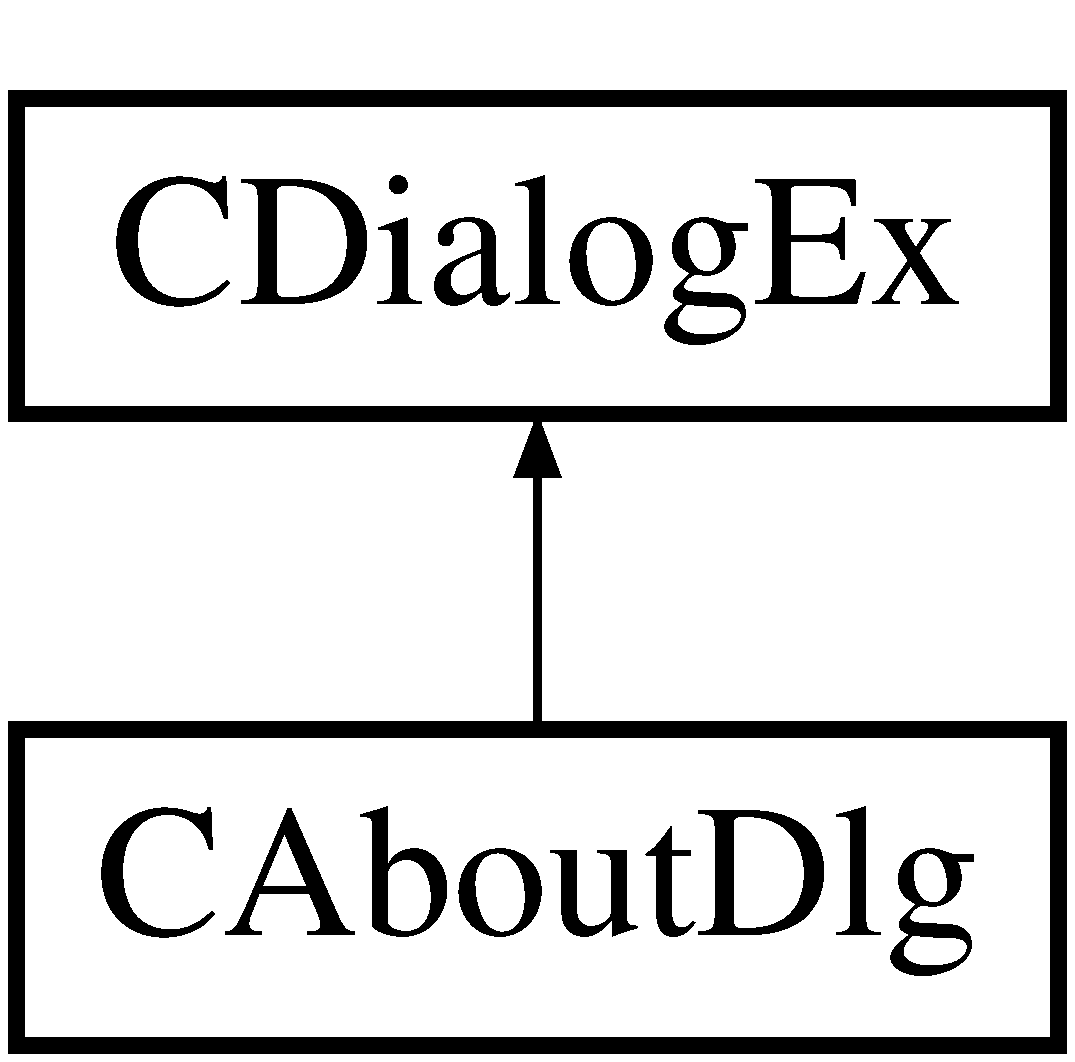
\includegraphics[height=2.000000cm]{class_c_about_dlg}
\end{center}
\end{figure}
\subsection*{Protected Member Functions}
\begin{DoxyCompactItemize}
\item 
\mbox{\Hypertarget{class_c_about_dlg_ab83db7484fec957282d7d5a21aed4df4}\label{class_c_about_dlg_ab83db7484fec957282d7d5a21aed4df4}} 
virtual void {\bfseries Do\+Data\+Exchange} (C\+Data\+Exchange $\ast$p\+DX)
\end{DoxyCompactItemize}


The documentation for this class was generated from the following file\+:\begin{DoxyCompactItemize}
\item 
Step2.\+cpp\end{DoxyCompactItemize}

\hypertarget{class_c_aquarium}{}\section{C\+Aquarium Class Reference}
\label{class_c_aquarium}\index{C\+Aquarium@{C\+Aquarium}}


{\ttfamily \#include $<$Aquarium.\+h$>$}

\subsection*{Public Member Functions}
\begin{DoxyCompactItemize}
\item 
\mbox{\hyperlink{class_c_aquarium_ab6ba8b1abd87437ff66748e82173a5a8}{C\+Aquarium}} ()
\item 
virtual \mbox{\hyperlink{class_c_aquarium_ab1baf78dc047af2b8cab8982e1446875}{$\sim$\+C\+Aquarium}} ()
\item 
void \mbox{\hyperlink{class_c_aquarium_a20b4899158d1ba4bc41217630d47e180}{On\+Draw}} (Gdiplus\+::\+Graphics $\ast$graphics)
\item 
void \mbox{\hyperlink{class_c_aquarium_a85063d05c147cf80f54182016fe12d64}{Add}} (std\+::shared\+\_\+ptr$<$ \mbox{\hyperlink{class_c_item}{C\+Item}} $>$ item)
\item 
std\+::shared\+\_\+ptr$<$ \mbox{\hyperlink{class_c_item}{C\+Item}} $>$ \mbox{\hyperlink{class_c_aquarium_a7129486467e76938fbc049723f9187f3}{Hit\+Test}} (int x, int y)
\item 
void \mbox{\hyperlink{class_c_aquarium_a2ee2a7d57d9f5d9996f9f9b468c98a2b}{Push\+To\+Front}} (std\+::shared\+\_\+ptr$<$ \mbox{\hyperlink{class_c_item}{C\+Item}} $>$ item)
\item 
bool \mbox{\hyperlink{class_c_aquarium_a111b3c61aa0cd3f8bdda1e2bc6b63ed1}{Killing}} (\mbox{\hyperlink{class_c_item}{C\+Item}} $\ast$item)
\item 
void \mbox{\hyperlink{class_c_aquarium_adc9e22446b161ec23acdef368cb8ac2e}{Clear}} ()
\item 
void \mbox{\hyperlink{class_c_aquarium_acace2b3a8c1ed29011d83ac8231c66d0}{Save}} (const std\+::wstring \&filename)
\item 
void \mbox{\hyperlink{class_c_aquarium_aeffc772356405adc8b79beba77c25d0f}{Update}} (double elapsed)
\item 
void \mbox{\hyperlink{class_c_aquarium_a21faac4da17cea923d8f7a5cebe45141}{Load}} (const std\+::wstring \&filename)
\item 
int \mbox{\hyperlink{class_c_aquarium_a002b101c76d468db423da85b9eb56210}{Get\+Width}} () const
\item 
int \mbox{\hyperlink{class_c_aquarium_a6553dfa3238a4e731dbdbe0ccd6ce956}{Get\+Height}} () const
\end{DoxyCompactItemize}


\subsection{Detailed Description}
Represents an aquarium 

\subsection{Constructor \& Destructor Documentation}
\mbox{\Hypertarget{class_c_aquarium_ab6ba8b1abd87437ff66748e82173a5a8}\label{class_c_aquarium_ab6ba8b1abd87437ff66748e82173a5a8}} 
\index{C\+Aquarium@{C\+Aquarium}!C\+Aquarium@{C\+Aquarium}}
\index{C\+Aquarium@{C\+Aquarium}!C\+Aquarium@{C\+Aquarium}}
\subsubsection{\texorpdfstring{C\+Aquarium()}{CAquarium()}}
{\footnotesize\ttfamily C\+Aquarium\+::\+C\+Aquarium (\begin{DoxyParamCaption}{ }\end{DoxyParamCaption})}

Constructor \mbox{\Hypertarget{class_c_aquarium_ab1baf78dc047af2b8cab8982e1446875}\label{class_c_aquarium_ab1baf78dc047af2b8cab8982e1446875}} 
\index{C\+Aquarium@{C\+Aquarium}!````~C\+Aquarium@{$\sim$\+C\+Aquarium}}
\index{````~C\+Aquarium@{$\sim$\+C\+Aquarium}!C\+Aquarium@{C\+Aquarium}}
\subsubsection{\texorpdfstring{$\sim$\+C\+Aquarium()}{~CAquarium()}}
{\footnotesize\ttfamily C\+Aquarium\+::$\sim$\+C\+Aquarium (\begin{DoxyParamCaption}{ }\end{DoxyParamCaption})\hspace{0.3cm}{\ttfamily [virtual]}}

Destructor 

\subsection{Member Function Documentation}
\mbox{\Hypertarget{class_c_aquarium_a85063d05c147cf80f54182016fe12d64}\label{class_c_aquarium_a85063d05c147cf80f54182016fe12d64}} 
\index{C\+Aquarium@{C\+Aquarium}!Add@{Add}}
\index{Add@{Add}!C\+Aquarium@{C\+Aquarium}}
\subsubsection{\texorpdfstring{Add()}{Add()}}
{\footnotesize\ttfamily void C\+Aquarium\+::\+Add (\begin{DoxyParamCaption}\item[{std\+::shared\+\_\+ptr$<$ \mbox{\hyperlink{class_c_item}{C\+Item}} $>$}]{item }\end{DoxyParamCaption})}

Add an item to the aquarium 
\begin{DoxyParams}{Parameters}
{\em item} & New item to add \\
\hline
\end{DoxyParams}
\mbox{\Hypertarget{class_c_aquarium_adc9e22446b161ec23acdef368cb8ac2e}\label{class_c_aquarium_adc9e22446b161ec23acdef368cb8ac2e}} 
\index{C\+Aquarium@{C\+Aquarium}!Clear@{Clear}}
\index{Clear@{Clear}!C\+Aquarium@{C\+Aquarium}}
\subsubsection{\texorpdfstring{Clear()}{Clear()}}
{\footnotesize\ttfamily void C\+Aquarium\+::\+Clear (\begin{DoxyParamCaption}{ }\end{DoxyParamCaption})}

Clear the aquarium data.

Deletes all known items in the aquarium. \mbox{\Hypertarget{class_c_aquarium_a6553dfa3238a4e731dbdbe0ccd6ce956}\label{class_c_aquarium_a6553dfa3238a4e731dbdbe0ccd6ce956}} 
\index{C\+Aquarium@{C\+Aquarium}!Get\+Height@{Get\+Height}}
\index{Get\+Height@{Get\+Height}!C\+Aquarium@{C\+Aquarium}}
\subsubsection{\texorpdfstring{Get\+Height()}{GetHeight()}}
{\footnotesize\ttfamily int C\+Aquarium\+::\+Get\+Height (\begin{DoxyParamCaption}{ }\end{DoxyParamCaption}) const\hspace{0.3cm}{\ttfamily [inline]}}

Get the height of the aquarium \begin{DoxyReturn}{Returns}
Aquarium height 
\end{DoxyReturn}
\mbox{\Hypertarget{class_c_aquarium_a002b101c76d468db423da85b9eb56210}\label{class_c_aquarium_a002b101c76d468db423da85b9eb56210}} 
\index{C\+Aquarium@{C\+Aquarium}!Get\+Width@{Get\+Width}}
\index{Get\+Width@{Get\+Width}!C\+Aquarium@{C\+Aquarium}}
\subsubsection{\texorpdfstring{Get\+Width()}{GetWidth()}}
{\footnotesize\ttfamily int C\+Aquarium\+::\+Get\+Width (\begin{DoxyParamCaption}{ }\end{DoxyParamCaption}) const\hspace{0.3cm}{\ttfamily [inline]}}

Get the width of the aquarium \begin{DoxyReturn}{Returns}
Aquarium width 
\end{DoxyReturn}
\mbox{\Hypertarget{class_c_aquarium_a7129486467e76938fbc049723f9187f3}\label{class_c_aquarium_a7129486467e76938fbc049723f9187f3}} 
\index{C\+Aquarium@{C\+Aquarium}!Hit\+Test@{Hit\+Test}}
\index{Hit\+Test@{Hit\+Test}!C\+Aquarium@{C\+Aquarium}}
\subsubsection{\texorpdfstring{Hit\+Test()}{HitTest()}}
{\footnotesize\ttfamily std\+::shared\+\_\+ptr$<$ \mbox{\hyperlink{class_c_item}{C\+Item}} $>$ C\+Aquarium\+::\+Hit\+Test (\begin{DoxyParamCaption}\item[{int}]{x,  }\item[{int}]{y }\end{DoxyParamCaption})}

Test an x,y click location to see if it clicked on some item in the aquarium. 
\begin{DoxyParams}{Parameters}
{\em x} & X location \\
\hline
{\em y} & Y location \\
\hline
\end{DoxyParams}
\begin{DoxyReturn}{Returns}
Pointer to item we clicked on or nullptr if none. 
\end{DoxyReturn}
\mbox{\Hypertarget{class_c_aquarium_a111b3c61aa0cd3f8bdda1e2bc6b63ed1}\label{class_c_aquarium_a111b3c61aa0cd3f8bdda1e2bc6b63ed1}} 
\index{C\+Aquarium@{C\+Aquarium}!Killing@{Killing}}
\index{Killing@{Killing}!C\+Aquarium@{C\+Aquarium}}
\subsubsection{\texorpdfstring{Killing()}{Killing()}}
{\footnotesize\ttfamily bool C\+Aquarium\+::\+Killing (\begin{DoxyParamCaption}\item[{\mbox{\hyperlink{class_c_item}{C\+Item}} $\ast$}]{eater }\end{DoxyParamCaption})}

We are passed a pointer to a fish that eats. We check to see if there are any fish it is currently over. If so, eat them! 
\begin{DoxyParams}{Parameters}
{\em item} & Item we are testing \\
\hline
{\em eater} & is the karp \\
\hline
\end{DoxyParams}
\begin{DoxyReturn}{Returns}
true if a fish is eaten 
\end{DoxyReturn}
\mbox{\Hypertarget{class_c_aquarium_a21faac4da17cea923d8f7a5cebe45141}\label{class_c_aquarium_a21faac4da17cea923d8f7a5cebe45141}} 
\index{C\+Aquarium@{C\+Aquarium}!Load@{Load}}
\index{Load@{Load}!C\+Aquarium@{C\+Aquarium}}
\subsubsection{\texorpdfstring{Load()}{Load()}}
{\footnotesize\ttfamily void C\+Aquarium\+::\+Load (\begin{DoxyParamCaption}\item[{const std\+::wstring \&}]{filename }\end{DoxyParamCaption})}

Load the aquarium from a .aqua X\+ML file.

Opens the X\+ML file and reads the nodes, creating items as appropriate.


\begin{DoxyParams}{Parameters}
{\em filename} & The filename of the file to load the aquarium from. \\
\hline
\end{DoxyParams}
\mbox{\Hypertarget{class_c_aquarium_a20b4899158d1ba4bc41217630d47e180}\label{class_c_aquarium_a20b4899158d1ba4bc41217630d47e180}} 
\index{C\+Aquarium@{C\+Aquarium}!On\+Draw@{On\+Draw}}
\index{On\+Draw@{On\+Draw}!C\+Aquarium@{C\+Aquarium}}
\subsubsection{\texorpdfstring{On\+Draw()}{OnDraw()}}
{\footnotesize\ttfamily void C\+Aquarium\+::\+On\+Draw (\begin{DoxyParamCaption}\item[{Gdiplus\+::\+Graphics $\ast$}]{graphics }\end{DoxyParamCaption})}

Draw the aquarium 
\begin{DoxyParams}{Parameters}
{\em graphics} & The G\+D\+I+ graphics context to draw on \\
\hline
\end{DoxyParams}
\mbox{\Hypertarget{class_c_aquarium_a2ee2a7d57d9f5d9996f9f9b468c98a2b}\label{class_c_aquarium_a2ee2a7d57d9f5d9996f9f9b468c98a2b}} 
\index{C\+Aquarium@{C\+Aquarium}!Push\+To\+Front@{Push\+To\+Front}}
\index{Push\+To\+Front@{Push\+To\+Front}!C\+Aquarium@{C\+Aquarium}}
\subsubsection{\texorpdfstring{Push\+To\+Front()}{PushToFront()}}
{\footnotesize\ttfamily void C\+Aquarium\+::\+Push\+To\+Front (\begin{DoxyParamCaption}\item[{std\+::shared\+\_\+ptr$<$ \mbox{\hyperlink{class_c_item}{C\+Item}} $>$}]{item }\end{DoxyParamCaption})}

Function to push to front of list 
\begin{DoxyParams}{Parameters}
{\em item} & \\
\hline
\end{DoxyParams}
\mbox{\Hypertarget{class_c_aquarium_acace2b3a8c1ed29011d83ac8231c66d0}\label{class_c_aquarium_acace2b3a8c1ed29011d83ac8231c66d0}} 
\index{C\+Aquarium@{C\+Aquarium}!Save@{Save}}
\index{Save@{Save}!C\+Aquarium@{C\+Aquarium}}
\subsubsection{\texorpdfstring{Save()}{Save()}}
{\footnotesize\ttfamily void C\+Aquarium\+::\+Save (\begin{DoxyParamCaption}\item[{const std\+::wstring \&}]{filename }\end{DoxyParamCaption})}

Save the aquarium as a .aqua X\+ML file.

Open an X\+ML file and stream the aquarium data to it.


\begin{DoxyParams}{Parameters}
{\em filename} & The filename of the file to save the aquarium to \\
\hline
\end{DoxyParams}
\mbox{\Hypertarget{class_c_aquarium_aeffc772356405adc8b79beba77c25d0f}\label{class_c_aquarium_aeffc772356405adc8b79beba77c25d0f}} 
\index{C\+Aquarium@{C\+Aquarium}!Update@{Update}}
\index{Update@{Update}!C\+Aquarium@{C\+Aquarium}}
\subsubsection{\texorpdfstring{Update()}{Update()}}
{\footnotesize\ttfamily void C\+Aquarium\+::\+Update (\begin{DoxyParamCaption}\item[{double}]{elapsed }\end{DoxyParamCaption})}

Handle updates for animation 
\begin{DoxyParams}{Parameters}
{\em elapsed} & The time since the last update \\
\hline
\end{DoxyParams}


The documentation for this class was generated from the following files\+:\begin{DoxyCompactItemize}
\item 
\mbox{\hyperlink{_aquarium_8h}{Aquarium.\+h}}\item 
\mbox{\hyperlink{_aquarium_8cpp}{Aquarium.\+cpp}}\end{DoxyCompactItemize}

\hypertarget{class_c_child_view}{}\section{C\+Child\+View Class Reference}
\label{class_c_child_view}\index{C\+Child\+View@{C\+Child\+View}}


{\ttfamily \#include $<$Child\+View.\+h$>$}

Inheritance diagram for C\+Child\+View\+:\begin{figure}[H]
\begin{center}
\leavevmode
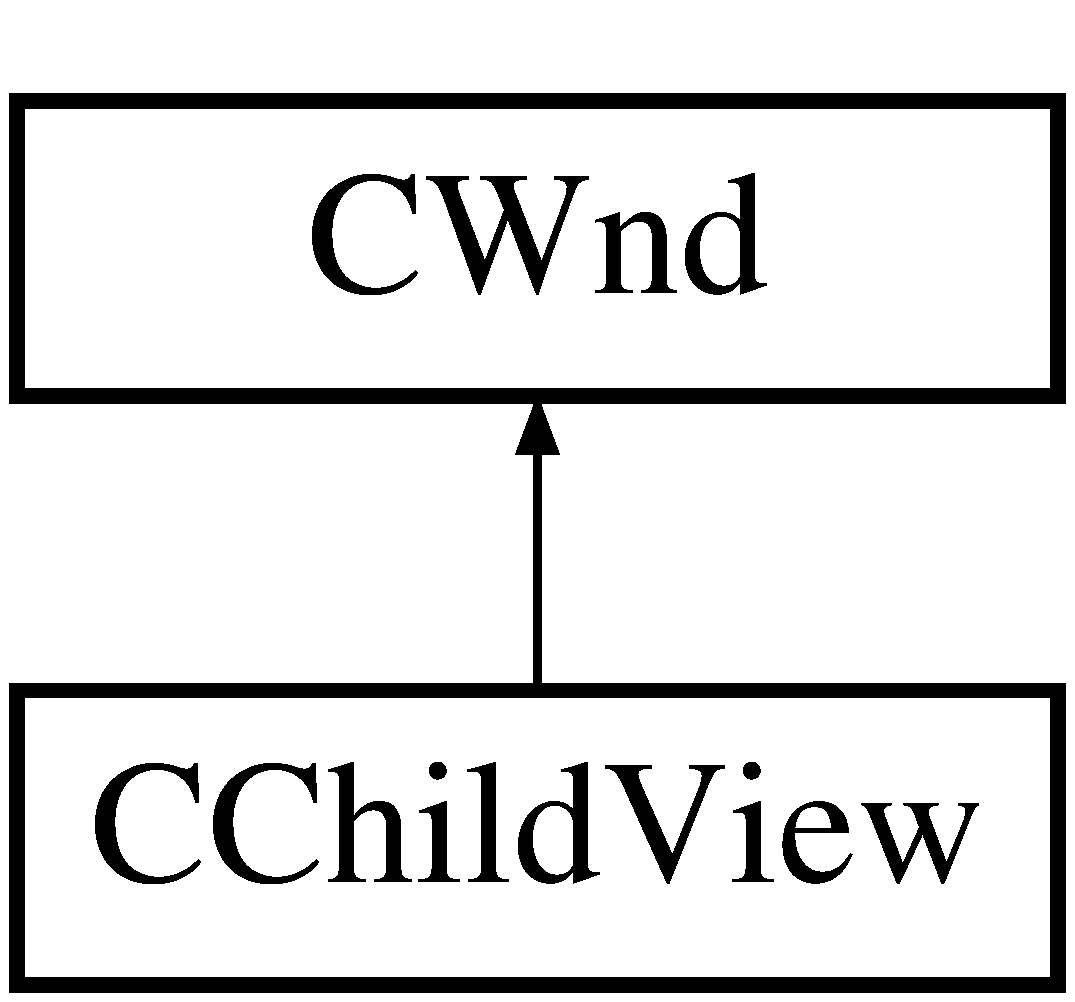
\includegraphics[height=2.000000cm]{class_c_child_view}
\end{center}
\end{figure}
\subsection*{Public Member Functions}
\begin{DoxyCompactItemize}
\item 
\mbox{\hyperlink{class_c_child_view_aff5af7c162c10755edbe58f260ded6d4}{C\+Child\+View}} ()
\item 
virtual \mbox{\hyperlink{class_c_child_view_a5b033b5e0a130950719a173b86418698}{$\sim$\+C\+Child\+View}} ()
\item 
afx\+\_\+msg void \mbox{\hyperlink{class_c_child_view_ad05faefbdb17d1c73f85de75b01a1ac1}{On\+Addfish\+Betafish}} ()
\item 
afx\+\_\+msg void \mbox{\hyperlink{class_c_child_view_ad3cb2f8d9fa9a6fb06989513dee5a8bc}{On\+Mouse\+Move}} (U\+I\+NT n\+Flags, C\+Point point)
\item 
afx\+\_\+msg void \mbox{\hyperlink{class_c_child_view_af513a57c45ce8b9dcc09dd934e228534}{On\+L\+Button\+Down}} (U\+I\+NT n\+Flags, C\+Point point)
\item 
afx\+\_\+msg void \mbox{\hyperlink{class_c_child_view_ae81948a77ebf3744bd0f9449af57ee21}{On\+L\+Button\+Up}} (U\+I\+NT n\+Flags, C\+Point point)
\item 
afx\+\_\+msg B\+O\+OL \mbox{\hyperlink{class_c_child_view_a6060e6d09d522d345dcee5a01d41c1f0}{On\+Erase\+Bkgnd}} (C\+DC $\ast$p\+DC)
\item 
afx\+\_\+msg void \mbox{\hyperlink{class_c_child_view_acb27b77bb4d6f4997c7d2d94f1a4e14c}{On\+Addfish\+Doryfish}} ()
\item 
afx\+\_\+msg void \mbox{\hyperlink{class_c_child_view_a6fddae71d821dd64cfae1359e8a33a62}{On\+Addfish\+Nemofish}} ()
\item 
afx\+\_\+msg void \mbox{\hyperlink{class_c_child_view_a0d3175bb87c2e24572d6c0364abebd07}{On\+Addfish\+Killerkarp}} ()
\item 
afx\+\_\+msg void \mbox{\hyperlink{class_c_child_view_aaf8f6acf9df7bdfa17f9dfcfa60d7883}{On\+Adddecor\+Decorcastle}} ()
\item 
afx\+\_\+msg void \mbox{\hyperlink{class_c_child_view_a2f79325c40f3a93227e60498b2135785}{On\+File\+Saveas}} ()
\item 
afx\+\_\+msg void \mbox{\hyperlink{class_c_child_view_a6e69d915eea1631da5f8a8d8d5a2c101}{On\+File\+Open32780}} ()
\item 
\mbox{\Hypertarget{class_c_child_view_a4c6bb8bd631cee84bb80c948f3d6d98a}\label{class_c_child_view_a4c6bb8bd631cee84bb80c948f3d6d98a}} 
afx\+\_\+msg void {\bfseries On\+Timer} (U\+I\+N\+T\+\_\+\+P\+TR n\+I\+D\+Event)
\end{DoxyCompactItemize}
\subsection*{Protected Member Functions}
\begin{DoxyCompactItemize}
\item 
afx\+\_\+msg void \mbox{\hyperlink{class_c_child_view_a8ea6d42631a4f9f446923ff864b239ab}{On\+Paint}} ()
\item 
\mbox{\Hypertarget{class_c_child_view_a072cbcba60255377ac9d82aed9a14ce8}\label{class_c_child_view_a072cbcba60255377ac9d82aed9a14ce8}} 
virtual B\+O\+OL {\bfseries Pre\+Create\+Window} (C\+R\+E\+A\+T\+E\+S\+T\+R\+U\+CT \&cs)
\end{DoxyCompactItemize}


\subsection{Detailed Description}
The child window our program draws in. 

\subsection{Constructor \& Destructor Documentation}
\mbox{\Hypertarget{class_c_child_view_aff5af7c162c10755edbe58f260ded6d4}\label{class_c_child_view_aff5af7c162c10755edbe58f260ded6d4}} 
\index{C\+Child\+View@{C\+Child\+View}!C\+Child\+View@{C\+Child\+View}}
\index{C\+Child\+View@{C\+Child\+View}!C\+Child\+View@{C\+Child\+View}}
\subsubsection{\texorpdfstring{C\+Child\+View()}{CChildView()}}
{\footnotesize\ttfamily C\+Child\+View\+::\+C\+Child\+View (\begin{DoxyParamCaption}{ }\end{DoxyParamCaption})}

Constructor \mbox{\Hypertarget{class_c_child_view_a5b033b5e0a130950719a173b86418698}\label{class_c_child_view_a5b033b5e0a130950719a173b86418698}} 
\index{C\+Child\+View@{C\+Child\+View}!````~C\+Child\+View@{$\sim$\+C\+Child\+View}}
\index{````~C\+Child\+View@{$\sim$\+C\+Child\+View}!C\+Child\+View@{C\+Child\+View}}
\subsubsection{\texorpdfstring{$\sim$\+C\+Child\+View()}{~CChildView()}}
{\footnotesize\ttfamily C\+Child\+View\+::$\sim$\+C\+Child\+View (\begin{DoxyParamCaption}{ }\end{DoxyParamCaption})\hspace{0.3cm}{\ttfamily [virtual]}}

Destructor 

\subsection{Member Function Documentation}
\mbox{\Hypertarget{class_c_child_view_aaf8f6acf9df7bdfa17f9dfcfa60d7883}\label{class_c_child_view_aaf8f6acf9df7bdfa17f9dfcfa60d7883}} 
\index{C\+Child\+View@{C\+Child\+View}!On\+Adddecor\+Decorcastle@{On\+Adddecor\+Decorcastle}}
\index{On\+Adddecor\+Decorcastle@{On\+Adddecor\+Decorcastle}!C\+Child\+View@{C\+Child\+View}}
\subsubsection{\texorpdfstring{On\+Adddecor\+Decorcastle()}{OnAdddecorDecorcastle()}}
{\footnotesize\ttfamily void C\+Child\+View\+::\+On\+Adddecor\+Decorcastle (\begin{DoxyParamCaption}{ }\end{DoxyParamCaption})}

Castle event handler for menu option. \mbox{\Hypertarget{class_c_child_view_ad05faefbdb17d1c73f85de75b01a1ac1}\label{class_c_child_view_ad05faefbdb17d1c73f85de75b01a1ac1}} 
\index{C\+Child\+View@{C\+Child\+View}!On\+Addfish\+Betafish@{On\+Addfish\+Betafish}}
\index{On\+Addfish\+Betafish@{On\+Addfish\+Betafish}!C\+Child\+View@{C\+Child\+View}}
\subsubsection{\texorpdfstring{On\+Addfish\+Betafish()}{OnAddfishBetafish()}}
{\footnotesize\ttfamily void C\+Child\+View\+::\+On\+Addfish\+Betafish (\begin{DoxyParamCaption}{ }\end{DoxyParamCaption})}

Function to add on a Beta Fish \mbox{\Hypertarget{class_c_child_view_acb27b77bb4d6f4997c7d2d94f1a4e14c}\label{class_c_child_view_acb27b77bb4d6f4997c7d2d94f1a4e14c}} 
\index{C\+Child\+View@{C\+Child\+View}!On\+Addfish\+Doryfish@{On\+Addfish\+Doryfish}}
\index{On\+Addfish\+Doryfish@{On\+Addfish\+Doryfish}!C\+Child\+View@{C\+Child\+View}}
\subsubsection{\texorpdfstring{On\+Addfish\+Doryfish()}{OnAddfishDoryfish()}}
{\footnotesize\ttfamily void C\+Child\+View\+::\+On\+Addfish\+Doryfish (\begin{DoxyParamCaption}{ }\end{DoxyParamCaption})}

Fish\+Dory event handler for menu option. \mbox{\Hypertarget{class_c_child_view_a0d3175bb87c2e24572d6c0364abebd07}\label{class_c_child_view_a0d3175bb87c2e24572d6c0364abebd07}} 
\index{C\+Child\+View@{C\+Child\+View}!On\+Addfish\+Killerkarp@{On\+Addfish\+Killerkarp}}
\index{On\+Addfish\+Killerkarp@{On\+Addfish\+Killerkarp}!C\+Child\+View@{C\+Child\+View}}
\subsubsection{\texorpdfstring{On\+Addfish\+Killerkarp()}{OnAddfishKillerkarp()}}
{\footnotesize\ttfamily void C\+Child\+View\+::\+On\+Addfish\+Killerkarp (\begin{DoxyParamCaption}{ }\end{DoxyParamCaption})}

Carp event handler for menu option. \mbox{\Hypertarget{class_c_child_view_a6fddae71d821dd64cfae1359e8a33a62}\label{class_c_child_view_a6fddae71d821dd64cfae1359e8a33a62}} 
\index{C\+Child\+View@{C\+Child\+View}!On\+Addfish\+Nemofish@{On\+Addfish\+Nemofish}}
\index{On\+Addfish\+Nemofish@{On\+Addfish\+Nemofish}!C\+Child\+View@{C\+Child\+View}}
\subsubsection{\texorpdfstring{On\+Addfish\+Nemofish()}{OnAddfishNemofish()}}
{\footnotesize\ttfamily void C\+Child\+View\+::\+On\+Addfish\+Nemofish (\begin{DoxyParamCaption}{ }\end{DoxyParamCaption})}

Fish\+Nemo event handler for menu option. \mbox{\Hypertarget{class_c_child_view_a6060e6d09d522d345dcee5a01d41c1f0}\label{class_c_child_view_a6060e6d09d522d345dcee5a01d41c1f0}} 
\index{C\+Child\+View@{C\+Child\+View}!On\+Erase\+Bkgnd@{On\+Erase\+Bkgnd}}
\index{On\+Erase\+Bkgnd@{On\+Erase\+Bkgnd}!C\+Child\+View@{C\+Child\+View}}
\subsubsection{\texorpdfstring{On\+Erase\+Bkgnd()}{OnEraseBkgnd()}}
{\footnotesize\ttfamily B\+O\+OL C\+Child\+View\+::\+On\+Erase\+Bkgnd (\begin{DoxyParamCaption}\item[{C\+DC $\ast$}]{p\+DC }\end{DoxyParamCaption})}

Erase the background

This is disabled to eliminate flicker 
\begin{DoxyParams}{Parameters}
{\em p\+DC} & Device context \\
\hline
\end{DoxyParams}
\begin{DoxyReturn}{Returns}
F\+A\+L\+SE 
\end{DoxyReturn}
\mbox{\Hypertarget{class_c_child_view_a6e69d915eea1631da5f8a8d8d5a2c101}\label{class_c_child_view_a6e69d915eea1631da5f8a8d8d5a2c101}} 
\index{C\+Child\+View@{C\+Child\+View}!On\+File\+Open32780@{On\+File\+Open32780}}
\index{On\+File\+Open32780@{On\+File\+Open32780}!C\+Child\+View@{C\+Child\+View}}
\subsubsection{\texorpdfstring{On\+File\+Open32780()}{OnFileOpen32780()}}
{\footnotesize\ttfamily void C\+Child\+View\+::\+On\+File\+Open32780 (\begin{DoxyParamCaption}{ }\end{DoxyParamCaption})}

This function is called when an File Open menu item is selected.

It loads the aquarium from a file. \mbox{\Hypertarget{class_c_child_view_a2f79325c40f3a93227e60498b2135785}\label{class_c_child_view_a2f79325c40f3a93227e60498b2135785}} 
\index{C\+Child\+View@{C\+Child\+View}!On\+File\+Saveas@{On\+File\+Saveas}}
\index{On\+File\+Saveas@{On\+File\+Saveas}!C\+Child\+View@{C\+Child\+View}}
\subsubsection{\texorpdfstring{On\+File\+Saveas()}{OnFileSaveas()}}
{\footnotesize\ttfamily void C\+Child\+View\+::\+On\+File\+Saveas (\begin{DoxyParamCaption}{ }\end{DoxyParamCaption})}

This function is called when an File Saveas menu item is selected.

It saves the aquarium as an X\+ML file. \mbox{\Hypertarget{class_c_child_view_af513a57c45ce8b9dcc09dd934e228534}\label{class_c_child_view_af513a57c45ce8b9dcc09dd934e228534}} 
\index{C\+Child\+View@{C\+Child\+View}!On\+L\+Button\+Down@{On\+L\+Button\+Down}}
\index{On\+L\+Button\+Down@{On\+L\+Button\+Down}!C\+Child\+View@{C\+Child\+View}}
\subsubsection{\texorpdfstring{On\+L\+Button\+Down()}{OnLButtonDown()}}
{\footnotesize\ttfamily void C\+Child\+View\+::\+On\+L\+Button\+Down (\begin{DoxyParamCaption}\item[{U\+I\+NT}]{n\+Flags,  }\item[{C\+Point}]{point }\end{DoxyParamCaption})}

Called when there is a left mouse button press 
\begin{DoxyParams}{Parameters}
{\em n\+Flags} & Flags associated with the mouse button press \\
\hline
{\em point} & Where the button was pressed \\
\hline
\end{DoxyParams}
\mbox{\Hypertarget{class_c_child_view_ae81948a77ebf3744bd0f9449af57ee21}\label{class_c_child_view_ae81948a77ebf3744bd0f9449af57ee21}} 
\index{C\+Child\+View@{C\+Child\+View}!On\+L\+Button\+Up@{On\+L\+Button\+Up}}
\index{On\+L\+Button\+Up@{On\+L\+Button\+Up}!C\+Child\+View@{C\+Child\+View}}
\subsubsection{\texorpdfstring{On\+L\+Button\+Up()}{OnLButtonUp()}}
{\footnotesize\ttfamily void C\+Child\+View\+::\+On\+L\+Button\+Up (\begin{DoxyParamCaption}\item[{U\+I\+NT}]{n\+Flags,  }\item[{C\+Point}]{point }\end{DoxyParamCaption})}

Called when the left mouse button is released 
\begin{DoxyParams}{Parameters}
{\em n\+Flags} & Flags associated with the mouse button release \\
\hline
{\em point} & Where the button was pressed \\
\hline
\end{DoxyParams}
\mbox{\Hypertarget{class_c_child_view_ad3cb2f8d9fa9a6fb06989513dee5a8bc}\label{class_c_child_view_ad3cb2f8d9fa9a6fb06989513dee5a8bc}} 
\index{C\+Child\+View@{C\+Child\+View}!On\+Mouse\+Move@{On\+Mouse\+Move}}
\index{On\+Mouse\+Move@{On\+Mouse\+Move}!C\+Child\+View@{C\+Child\+View}}
\subsubsection{\texorpdfstring{On\+Mouse\+Move()}{OnMouseMove()}}
{\footnotesize\ttfamily void C\+Child\+View\+::\+On\+Mouse\+Move (\begin{DoxyParamCaption}\item[{U\+I\+NT}]{n\+Flags,  }\item[{C\+Point}]{point }\end{DoxyParamCaption})}

Called when the mouse is moved 
\begin{DoxyParams}{Parameters}
{\em n\+Flags} & Flags associated with the mouse movement \\
\hline
{\em point} & Where the button was pressed \\
\hline
\end{DoxyParams}
\mbox{\Hypertarget{class_c_child_view_a8ea6d42631a4f9f446923ff864b239ab}\label{class_c_child_view_a8ea6d42631a4f9f446923ff864b239ab}} 
\index{C\+Child\+View@{C\+Child\+View}!On\+Paint@{On\+Paint}}
\index{On\+Paint@{On\+Paint}!C\+Child\+View@{C\+Child\+View}}
\subsubsection{\texorpdfstring{On\+Paint()}{OnPaint()}}
{\footnotesize\ttfamily void C\+Child\+View\+::\+On\+Paint (\begin{DoxyParamCaption}{ }\end{DoxyParamCaption})\hspace{0.3cm}{\ttfamily [protected]}}

This function is called to draw in the window.

This function is called in response to a drawing message whenever we need to redraw the window on the screen. It is responsible for painting the window. 

The documentation for this class was generated from the following files\+:\begin{DoxyCompactItemize}
\item 
\mbox{\hyperlink{_child_view_8h}{Child\+View.\+h}}\item 
\mbox{\hyperlink{_child_view_8cpp}{Child\+View.\+cpp}}\end{DoxyCompactItemize}

\hypertarget{class_c_decor_castle}{}\section{C\+Decor\+Castle Class Reference}
\label{class_c_decor_castle}\index{C\+Decor\+Castle@{C\+Decor\+Castle}}


{\ttfamily \#include $<$Decor\+Castle.\+h$>$}

Inheritance diagram for C\+Decor\+Castle\+:\begin{figure}[H]
\begin{center}
\leavevmode
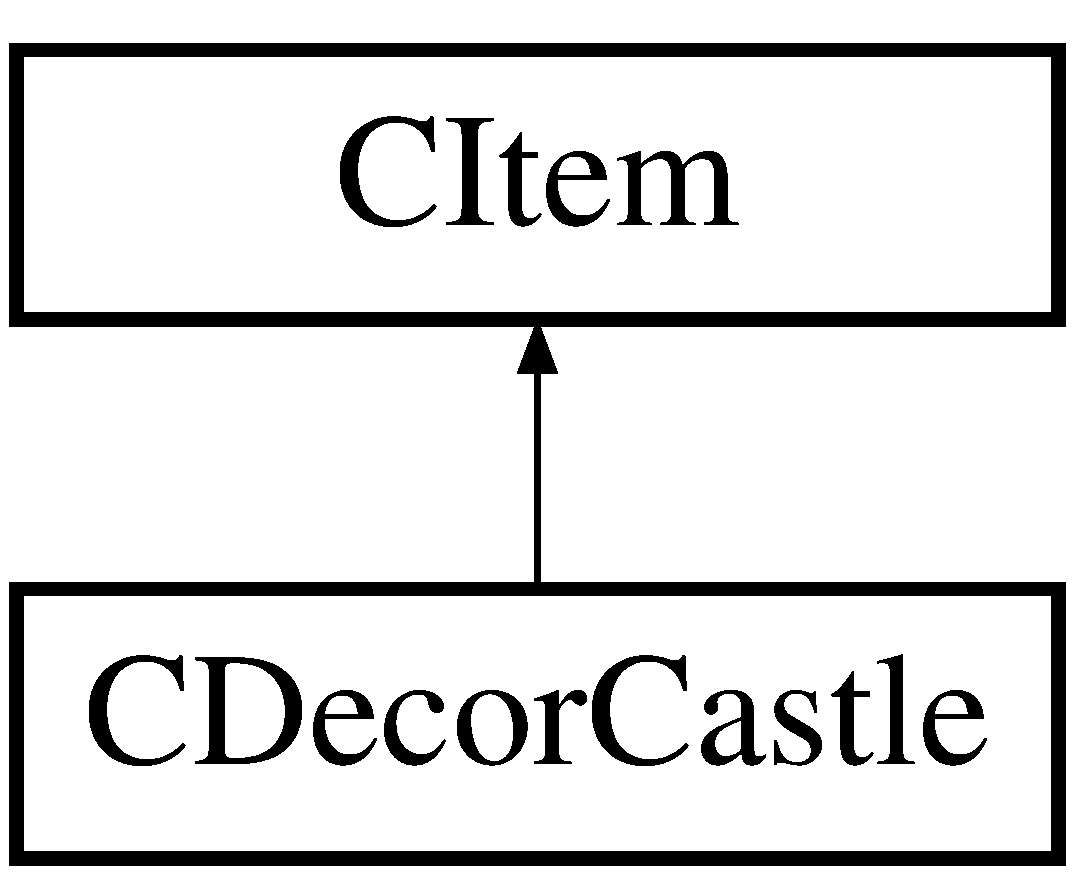
\includegraphics[height=2.000000cm]{class_c_decor_castle}
\end{center}
\end{figure}
\subsection*{Public Member Functions}
\begin{DoxyCompactItemize}
\item 
\mbox{\hyperlink{class_c_decor_castle_a9c88c926ea898a19ef6b726a722f39af}{C\+Decor\+Castle}} (\mbox{\hyperlink{class_c_aquarium}{C\+Aquarium}} $\ast$aquarium)
\item 
\mbox{\Hypertarget{class_c_decor_castle_a5f0d27e7013bc141525986d2bd6cd3f3}\label{class_c_decor_castle_a5f0d27e7013bc141525986d2bd6cd3f3}} 
\mbox{\hyperlink{class_c_decor_castle_a5f0d27e7013bc141525986d2bd6cd3f3}{C\+Decor\+Castle}} ()=delete
\begin{DoxyCompactList}\small\item\em Default Constructor. \end{DoxyCompactList}\item 
\mbox{\Hypertarget{class_c_decor_castle_a430a8ba95eb526bda2d966a63d11e73c}\label{class_c_decor_castle_a430a8ba95eb526bda2d966a63d11e73c}} 
\mbox{\hyperlink{class_c_decor_castle_a430a8ba95eb526bda2d966a63d11e73c}{C\+Decor\+Castle}} (const \mbox{\hyperlink{class_c_decor_castle}{C\+Decor\+Castle}} \&)=delete
\begin{DoxyCompactList}\small\item\em Copy constructor (disabled) \end{DoxyCompactList}\item 
virtual std\+::shared\+\_\+ptr$<$ \mbox{\hyperlink{classxmlnode_1_1_c_xml_node}{xmlnode\+::\+C\+Xml\+Node}} $>$ \mbox{\hyperlink{class_c_decor_castle_a83ecb7c898679e55dcafbc6492bc38d0}{Xml\+Save}} (const std\+::shared\+\_\+ptr$<$ \mbox{\hyperlink{classxmlnode_1_1_c_xml_node}{xmlnode\+::\+C\+Xml\+Node}} $>$ \&node) override
\item 
virtual \mbox{\hyperlink{class_c_decor_castle_a520ef2928c6d8a115200d64060b93c6f}{$\sim$\+C\+Decor\+Castle}} ()
\begin{DoxyCompactList}\small\item\em Destructor. \end{DoxyCompactList}\end{DoxyCompactItemize}
\subsection*{Additional Inherited Members}


\subsection{Detailed Description}
Implements a Decor Castle. 

\subsection{Constructor \& Destructor Documentation}
\mbox{\Hypertarget{class_c_decor_castle_a9c88c926ea898a19ef6b726a722f39af}\label{class_c_decor_castle_a9c88c926ea898a19ef6b726a722f39af}} 
\index{C\+Decor\+Castle@{C\+Decor\+Castle}!C\+Decor\+Castle@{C\+Decor\+Castle}}
\index{C\+Decor\+Castle@{C\+Decor\+Castle}!C\+Decor\+Castle@{C\+Decor\+Castle}}
\subsubsection{\texorpdfstring{C\+Decor\+Castle()}{CDecorCastle()}}
{\footnotesize\ttfamily C\+Decor\+Castle\+::\+C\+Decor\+Castle (\begin{DoxyParamCaption}\item[{\mbox{\hyperlink{class_c_aquarium}{C\+Aquarium}} $\ast$}]{aquarium }\end{DoxyParamCaption})}

Constructor 
\begin{DoxyParams}{Parameters}
{\em aquarium} & The aquarium this is a member of \\
\hline
\end{DoxyParams}
\mbox{\Hypertarget{class_c_decor_castle_a520ef2928c6d8a115200d64060b93c6f}\label{class_c_decor_castle_a520ef2928c6d8a115200d64060b93c6f}} 
\index{C\+Decor\+Castle@{C\+Decor\+Castle}!````~C\+Decor\+Castle@{$\sim$\+C\+Decor\+Castle}}
\index{````~C\+Decor\+Castle@{$\sim$\+C\+Decor\+Castle}!C\+Decor\+Castle@{C\+Decor\+Castle}}
\subsubsection{\texorpdfstring{$\sim$\+C\+Decor\+Castle()}{~CDecorCastle()}}
{\footnotesize\ttfamily C\+Decor\+Castle\+::$\sim$\+C\+Decor\+Castle (\begin{DoxyParamCaption}{ }\end{DoxyParamCaption})\hspace{0.3cm}{\ttfamily [virtual]}}



Destructor. 

Destructor 

\subsection{Member Function Documentation}
\mbox{\Hypertarget{class_c_decor_castle_a83ecb7c898679e55dcafbc6492bc38d0}\label{class_c_decor_castle_a83ecb7c898679e55dcafbc6492bc38d0}} 
\index{C\+Decor\+Castle@{C\+Decor\+Castle}!Xml\+Save@{Xml\+Save}}
\index{Xml\+Save@{Xml\+Save}!C\+Decor\+Castle@{C\+Decor\+Castle}}
\subsubsection{\texorpdfstring{Xml\+Save()}{XmlSave()}}
{\footnotesize\ttfamily std\+::shared\+\_\+ptr$<$ \mbox{\hyperlink{classxmlnode_1_1_c_xml_node}{xmlnode\+::\+C\+Xml\+Node}} $>$ C\+Decor\+Castle\+::\+Xml\+Save (\begin{DoxyParamCaption}\item[{const std\+::shared\+\_\+ptr$<$ \mbox{\hyperlink{classxmlnode_1_1_c_xml_node}{xmlnode\+::\+C\+Xml\+Node}} $>$ \&}]{node }\end{DoxyParamCaption})\hspace{0.3cm}{\ttfamily [override]}, {\ttfamily [virtual]}}

Save this item to an X\+ML node 
\begin{DoxyParams}{Parameters}
{\em node} & The node we are going to be a child of \\
\hline
\end{DoxyParams}


Reimplemented from \mbox{\hyperlink{class_c_item_a10584fa8e05d3abe125f95f0ceecdedd}{C\+Item}}.



The documentation for this class was generated from the following files\+:\begin{DoxyCompactItemize}
\item 
\mbox{\hyperlink{_decor_castle_8h}{Decor\+Castle.\+h}}\item 
Decor\+Castle.\+cpp\end{DoxyCompactItemize}

\hypertarget{class_c_fish}{}\section{C\+Fish Class Reference}
\label{class_c_fish}\index{C\+Fish@{C\+Fish}}


{\ttfamily \#include $<$Fish.\+h$>$}

Inheritance diagram for C\+Fish\+:\begin{figure}[H]
\begin{center}
\leavevmode
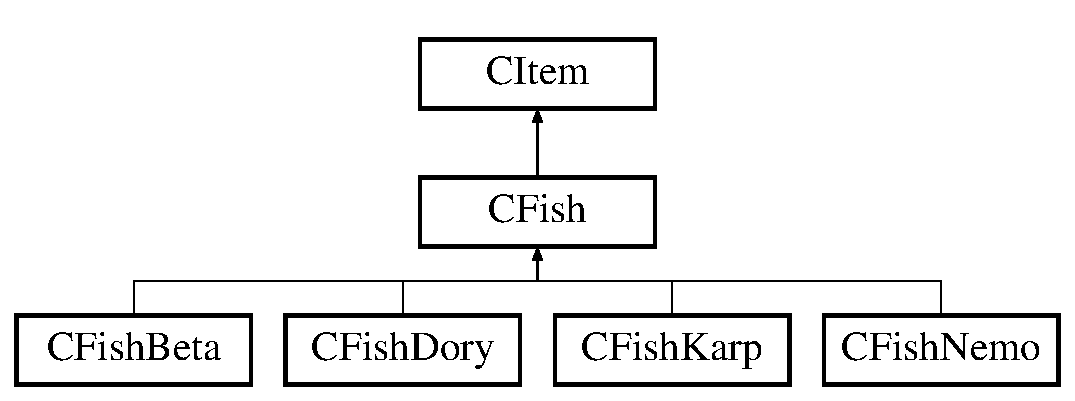
\includegraphics[height=3.000000cm]{class_c_fish}
\end{center}
\end{figure}
\subsection*{Public Member Functions}
\begin{DoxyCompactItemize}
\item 
\mbox{\Hypertarget{class_c_fish_ac4c190f887382bb976a3bca156010d60}\label{class_c_fish_ac4c190f887382bb976a3bca156010d60}} 
\mbox{\hyperlink{class_c_fish_ac4c190f887382bb976a3bca156010d60}{C\+Fish}} ()=delete
\begin{DoxyCompactList}\small\item\em Default constructor (disabled) \end{DoxyCompactList}\item 
\mbox{\Hypertarget{class_c_fish_a74ba012f126e8e105638cba899c5434b}\label{class_c_fish_a74ba012f126e8e105638cba899c5434b}} 
\mbox{\hyperlink{class_c_fish_a74ba012f126e8e105638cba899c5434b}{C\+Fish}} (const \mbox{\hyperlink{class_c_fish}{C\+Fish}} \&)=delete
\begin{DoxyCompactList}\small\item\em Copy constructor (disabled) \end{DoxyCompactList}\item 
std\+::shared\+\_\+ptr$<$ \mbox{\hyperlink{classxmlnode_1_1_c_xml_node}{xmlnode\+::\+C\+Xml\+Node}} $>$ \mbox{\hyperlink{class_c_fish_abfc997d2d755be8f94069c57e75a854b}{Xml\+Save}} (const std\+::shared\+\_\+ptr$<$ \mbox{\hyperlink{classxmlnode_1_1_c_xml_node}{xmlnode\+::\+C\+Xml\+Node}} $>$ \&node)
\item 
void \mbox{\hyperlink{class_c_fish_a997f243d89dd8c397597010eec4b611e}{Xml\+Load}} (const std\+::shared\+\_\+ptr$<$ \mbox{\hyperlink{classxmlnode_1_1_c_xml_node}{xmlnode\+::\+C\+Xml\+Node}} $>$ \&node) override
\item 
void \mbox{\hyperlink{class_c_fish_ab3d626359c6bcbb020583ddd19032447}{Change\+Speed}} (int SpeedX, int SpeedY)
\end{DoxyCompactItemize}
\subsection*{Protected Member Functions}
\begin{DoxyCompactItemize}
\item 
\mbox{\hyperlink{class_c_fish_a1daf95e31dfa4f045b67ea821b625275}{C\+Fish}} (\mbox{\hyperlink{class_c_aquarium}{C\+Aquarium}} $\ast$aquarium, const std\+::wstring \&filename)
\item 
void \mbox{\hyperlink{class_c_fish_a1f32288b28d3c1f186bd51cf8ac71aeb}{Update}} (double elapsed)
\end{DoxyCompactItemize}


\subsection{Detailed Description}
Base class for a fish This applies to all of the fish, but not the decor items in the aquarium. 

\subsection{Constructor \& Destructor Documentation}
\mbox{\Hypertarget{class_c_fish_a1daf95e31dfa4f045b67ea821b625275}\label{class_c_fish_a1daf95e31dfa4f045b67ea821b625275}} 
\index{C\+Fish@{C\+Fish}!C\+Fish@{C\+Fish}}
\index{C\+Fish@{C\+Fish}!C\+Fish@{C\+Fish}}
\subsubsection{\texorpdfstring{C\+Fish()}{CFish()}}
{\footnotesize\ttfamily C\+Fish\+::\+C\+Fish (\begin{DoxyParamCaption}\item[{\mbox{\hyperlink{class_c_aquarium}{C\+Aquarium}} $\ast$}]{aquarium,  }\item[{const std\+::wstring \&}]{filename }\end{DoxyParamCaption})\hspace{0.3cm}{\ttfamily [protected]}}

Constructor 
\begin{DoxyParams}{Parameters}
{\em aquarium} & The aquarium we are in \\
\hline
{\em filename} & Filename for the image we use \\
\hline
\end{DoxyParams}


\subsection{Member Function Documentation}
\mbox{\Hypertarget{class_c_fish_ab3d626359c6bcbb020583ddd19032447}\label{class_c_fish_ab3d626359c6bcbb020583ddd19032447}} 
\index{C\+Fish@{C\+Fish}!Change\+Speed@{Change\+Speed}}
\index{Change\+Speed@{Change\+Speed}!C\+Fish@{C\+Fish}}
\subsubsection{\texorpdfstring{Change\+Speed()}{ChangeSpeed()}}
{\footnotesize\ttfamily void C\+Fish\+::\+Change\+Speed (\begin{DoxyParamCaption}\item[{int}]{SpeedX,  }\item[{int}]{SpeedY }\end{DoxyParamCaption})}

Changes fish speed based on minimum and maximum speeds set. 
\begin{DoxyParams}{Parameters}
{\em SpeedX,SpeedY} & \\
\hline
\end{DoxyParams}
\mbox{\Hypertarget{class_c_fish_a1f32288b28d3c1f186bd51cf8ac71aeb}\label{class_c_fish_a1f32288b28d3c1f186bd51cf8ac71aeb}} 
\index{C\+Fish@{C\+Fish}!Update@{Update}}
\index{Update@{Update}!C\+Fish@{C\+Fish}}
\subsubsection{\texorpdfstring{Update()}{Update()}}
{\footnotesize\ttfamily void C\+Fish\+::\+Update (\begin{DoxyParamCaption}\item[{double}]{elapsed }\end{DoxyParamCaption})\hspace{0.3cm}{\ttfamily [protected]}, {\ttfamily [virtual]}}

Handle updates in time of our fish

This is called before we draw and allows us to move our fish. We add our speed times the amount of time that has elapsed. 
\begin{DoxyParams}{Parameters}
{\em elapsed} & Time elapsed since the class call \\
\hline
\end{DoxyParams}


Reimplemented from \mbox{\hyperlink{class_c_item_a0e88df0b5e12a93941dcec378797d0fe}{C\+Item}}.

\mbox{\Hypertarget{class_c_fish_a997f243d89dd8c397597010eec4b611e}\label{class_c_fish_a997f243d89dd8c397597010eec4b611e}} 
\index{C\+Fish@{C\+Fish}!Xml\+Load@{Xml\+Load}}
\index{Xml\+Load@{Xml\+Load}!C\+Fish@{C\+Fish}}
\subsubsection{\texorpdfstring{Xml\+Load()}{XmlLoad()}}
{\footnotesize\ttfamily void C\+Fish\+::\+Xml\+Load (\begin{DoxyParamCaption}\item[{const std\+::shared\+\_\+ptr$<$ \mbox{\hyperlink{classxmlnode_1_1_c_xml_node}{xmlnode\+::\+C\+Xml\+Node}} $>$ \&}]{node }\end{DoxyParamCaption})\hspace{0.3cm}{\ttfamily [override]}, {\ttfamily [virtual]}}

Load the attributes for an item node.

This is the base class version that loads the attributes common to all items. Override this to load custom attributes for specific items.


\begin{DoxyParams}{Parameters}
{\em node} & The Xml node we are loading the item from \\
\hline
\end{DoxyParams}


Reimplemented from \mbox{\hyperlink{class_c_item_ad0bad7d47a01ff133734b5498f9ca3bb}{C\+Item}}.

\mbox{\Hypertarget{class_c_fish_abfc997d2d755be8f94069c57e75a854b}\label{class_c_fish_abfc997d2d755be8f94069c57e75a854b}} 
\index{C\+Fish@{C\+Fish}!Xml\+Save@{Xml\+Save}}
\index{Xml\+Save@{Xml\+Save}!C\+Fish@{C\+Fish}}
\subsubsection{\texorpdfstring{Xml\+Save()}{XmlSave()}}
{\footnotesize\ttfamily std\+::shared\+\_\+ptr$<$ \mbox{\hyperlink{classxmlnode_1_1_c_xml_node}{xmlnode\+::\+C\+Xml\+Node}} $>$ C\+Fish\+::\+Xml\+Save (\begin{DoxyParamCaption}\item[{const std\+::shared\+\_\+ptr$<$ \mbox{\hyperlink{classxmlnode_1_1_c_xml_node}{xmlnode\+::\+C\+Xml\+Node}} $>$ \&}]{node }\end{DoxyParamCaption})\hspace{0.3cm}{\ttfamily [virtual]}}

Save this item to an X\+ML node 
\begin{DoxyParams}{Parameters}
{\em node} & The node we are going to be a child of \\
\hline
\end{DoxyParams}
\begin{DoxyReturn}{Returns}
xmlnode ptr 
\end{DoxyReturn}


Reimplemented from \mbox{\hyperlink{class_c_item_a10584fa8e05d3abe125f95f0ceecdedd}{C\+Item}}.



Reimplemented in \mbox{\hyperlink{class_c_fish_beta_a0be2886a531ede77bfa5338fec71d71b}{C\+Fish\+Beta}}, \mbox{\hyperlink{class_c_fish_nemo_ae9fd9446cd4852c9d9a78831bec0f32f}{C\+Fish\+Nemo}}, \mbox{\hyperlink{class_c_fish_dory_ac906b7f952cdbc52a72d1e87c9228ad9}{C\+Fish\+Dory}}, and \mbox{\hyperlink{class_c_fish_karp_a182d8cce606be73a981bd140aca64ba8}{C\+Fish\+Karp}}.



The documentation for this class was generated from the following files\+:\begin{DoxyCompactItemize}
\item 
Fish.\+h\item 
\mbox{\hyperlink{_fish_8cpp}{Fish.\+cpp}}\end{DoxyCompactItemize}

\hypertarget{class_c_fish_beta}{}\section{C\+Fish\+Beta Class Reference}
\label{class_c_fish_beta}\index{C\+Fish\+Beta@{C\+Fish\+Beta}}


{\ttfamily \#include $<$Fish\+Beta.\+h$>$}

Inheritance diagram for C\+Fish\+Beta\+:\begin{figure}[H]
\begin{center}
\leavevmode
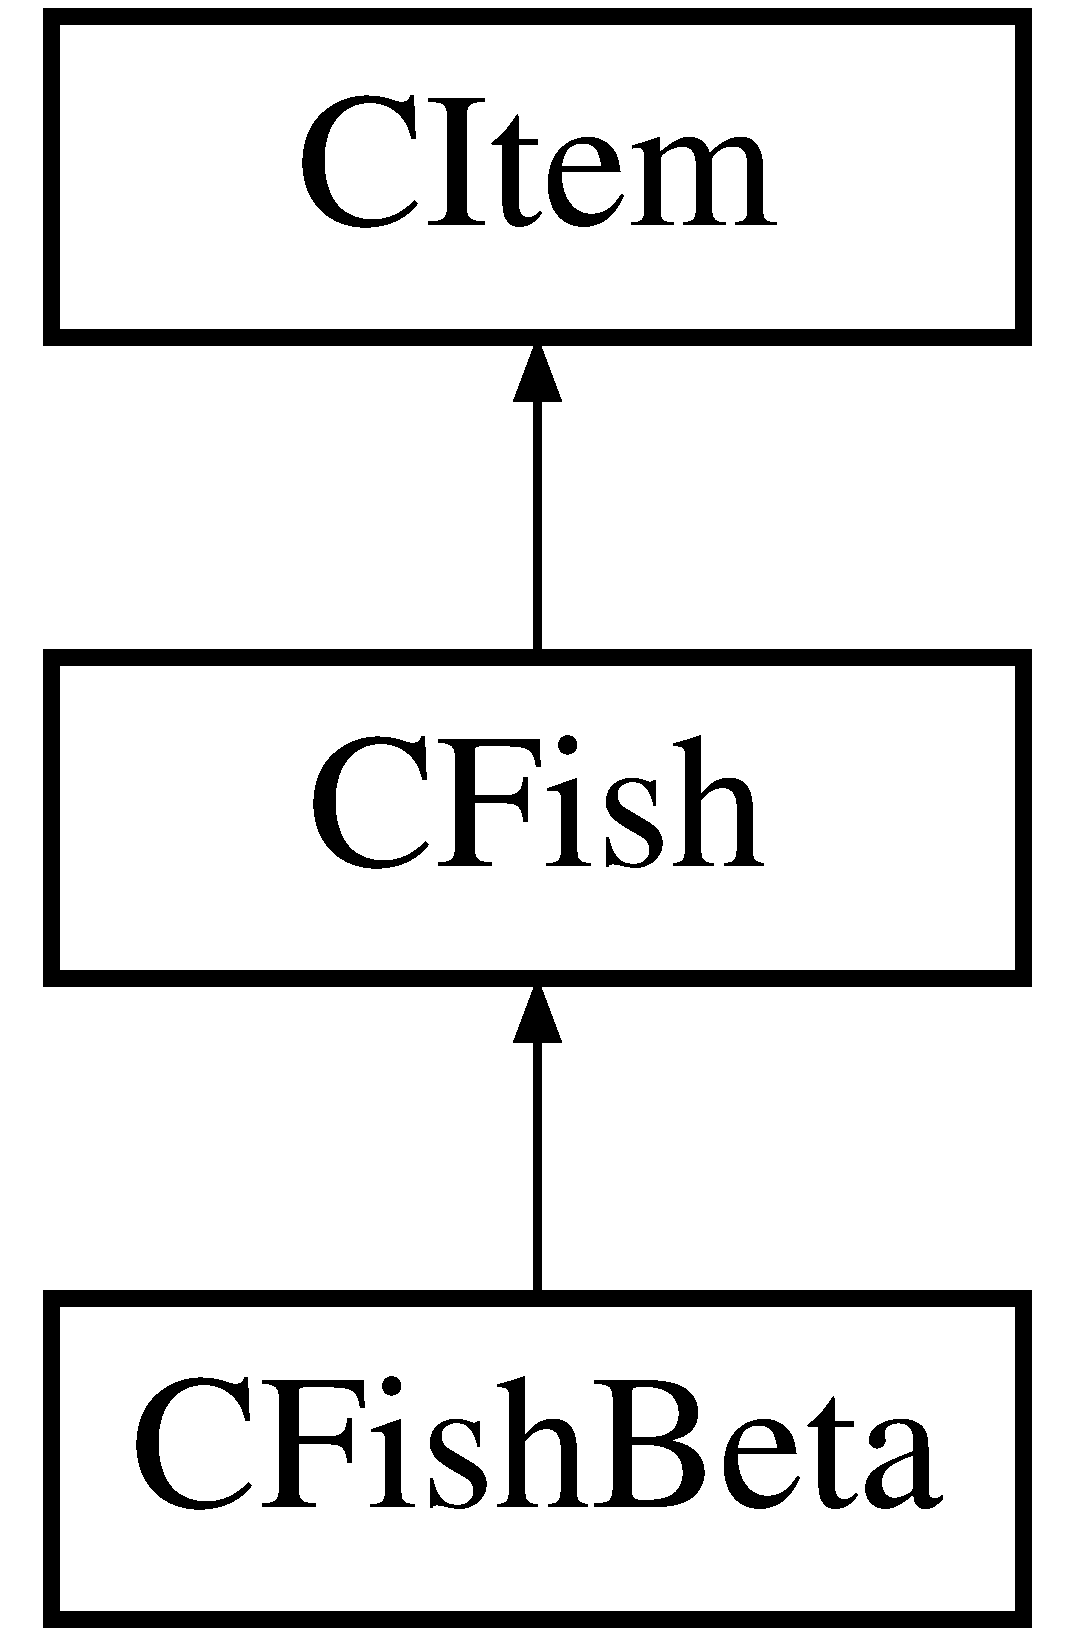
\includegraphics[height=3.000000cm]{class_c_fish_beta}
\end{center}
\end{figure}
\subsection*{Public Member Functions}
\begin{DoxyCompactItemize}
\item 
\mbox{\hyperlink{class_c_fish_beta_a021073e2e0034271cd7e776b1e3fed29}{C\+Fish\+Beta}} (\mbox{\hyperlink{class_c_aquarium}{C\+Aquarium}} $\ast$aquarium)
\item 
\mbox{\Hypertarget{class_c_fish_beta_a4e4d132618735adad44d04c9c40687ca}\label{class_c_fish_beta_a4e4d132618735adad44d04c9c40687ca}} 
\mbox{\hyperlink{class_c_fish_beta_a4e4d132618735adad44d04c9c40687ca}{C\+Fish\+Beta}} ()=delete
\begin{DoxyCompactList}\small\item\em Default constructor (disabled) \end{DoxyCompactList}\item 
\mbox{\Hypertarget{class_c_fish_beta_adbf3559baac135dff393729c51b1ab31}\label{class_c_fish_beta_adbf3559baac135dff393729c51b1ab31}} 
\mbox{\hyperlink{class_c_fish_beta_adbf3559baac135dff393729c51b1ab31}{C\+Fish\+Beta}} (const \mbox{\hyperlink{class_c_fish_beta}{C\+Fish\+Beta}} \&)=delete
\begin{DoxyCompactList}\small\item\em Copy constructor (disabled) \end{DoxyCompactList}\item 
virtual std\+::shared\+\_\+ptr$<$ \mbox{\hyperlink{classxmlnode_1_1_c_xml_node}{xmlnode\+::\+C\+Xml\+Node}} $>$ \mbox{\hyperlink{class_c_fish_beta_a0be2886a531ede77bfa5338fec71d71b}{Xml\+Save}} (const std\+::shared\+\_\+ptr$<$ \mbox{\hyperlink{classxmlnode_1_1_c_xml_node}{xmlnode\+::\+C\+Xml\+Node}} $>$ \&node) override
\item 
\mbox{\hyperlink{class_c_fish_beta_abd932894ad25a70f03c79c4f0f00fff4}{$\sim$\+C\+Fish\+Beta}} ()
\end{DoxyCompactItemize}
\subsection*{Additional Inherited Members}


\subsection{Detailed Description}
Implements a Beta fish 

\subsection{Constructor \& Destructor Documentation}
\mbox{\Hypertarget{class_c_fish_beta_a021073e2e0034271cd7e776b1e3fed29}\label{class_c_fish_beta_a021073e2e0034271cd7e776b1e3fed29}} 
\index{C\+Fish\+Beta@{C\+Fish\+Beta}!C\+Fish\+Beta@{C\+Fish\+Beta}}
\index{C\+Fish\+Beta@{C\+Fish\+Beta}!C\+Fish\+Beta@{C\+Fish\+Beta}}
\subsubsection{\texorpdfstring{C\+Fish\+Beta()}{CFishBeta()}}
{\footnotesize\ttfamily C\+Fish\+Beta\+::\+C\+Fish\+Beta (\begin{DoxyParamCaption}\item[{\mbox{\hyperlink{class_c_aquarium}{C\+Aquarium}} $\ast$}]{aquarium }\end{DoxyParamCaption})}

Constructor 
\begin{DoxyParams}{Parameters}
{\em aquarium} & The aquarium this is a member of \\
\hline
\end{DoxyParams}
\mbox{\Hypertarget{class_c_fish_beta_abd932894ad25a70f03c79c4f0f00fff4}\label{class_c_fish_beta_abd932894ad25a70f03c79c4f0f00fff4}} 
\index{C\+Fish\+Beta@{C\+Fish\+Beta}!````~C\+Fish\+Beta@{$\sim$\+C\+Fish\+Beta}}
\index{````~C\+Fish\+Beta@{$\sim$\+C\+Fish\+Beta}!C\+Fish\+Beta@{C\+Fish\+Beta}}
\subsubsection{\texorpdfstring{$\sim$\+C\+Fish\+Beta()}{~CFishBeta()}}
{\footnotesize\ttfamily C\+Fish\+Beta\+::$\sim$\+C\+Fish\+Beta (\begin{DoxyParamCaption}{ }\end{DoxyParamCaption})}

Destructor 

\subsection{Member Function Documentation}
\mbox{\Hypertarget{class_c_fish_beta_a0be2886a531ede77bfa5338fec71d71b}\label{class_c_fish_beta_a0be2886a531ede77bfa5338fec71d71b}} 
\index{C\+Fish\+Beta@{C\+Fish\+Beta}!Xml\+Save@{Xml\+Save}}
\index{Xml\+Save@{Xml\+Save}!C\+Fish\+Beta@{C\+Fish\+Beta}}
\subsubsection{\texorpdfstring{Xml\+Save()}{XmlSave()}}
{\footnotesize\ttfamily std\+::shared\+\_\+ptr$<$ \mbox{\hyperlink{classxmlnode_1_1_c_xml_node}{xmlnode\+::\+C\+Xml\+Node}} $>$ C\+Fish\+Beta\+::\+Xml\+Save (\begin{DoxyParamCaption}\item[{const std\+::shared\+\_\+ptr$<$ \mbox{\hyperlink{classxmlnode_1_1_c_xml_node}{xmlnode\+::\+C\+Xml\+Node}} $>$ \&}]{node }\end{DoxyParamCaption})\hspace{0.3cm}{\ttfamily [override]}, {\ttfamily [virtual]}}

Save this item to an X\+ML node 
\begin{DoxyParams}{Parameters}
{\em node} & The node we are going to be a child of \\
\hline
\end{DoxyParams}


Reimplemented from \mbox{\hyperlink{class_c_fish_abfc997d2d755be8f94069c57e75a854b}{C\+Fish}}.



The documentation for this class was generated from the following files\+:\begin{DoxyCompactItemize}
\item 
\mbox{\hyperlink{_fish_beta_8h}{Fish\+Beta.\+h}}\item 
\mbox{\hyperlink{_fish_beta_8cpp}{Fish\+Beta.\+cpp}}\end{DoxyCompactItemize}

\hypertarget{class_c_fish_dory}{}\section{C\+Fish\+Dory Class Reference}
\label{class_c_fish_dory}\index{C\+Fish\+Dory@{C\+Fish\+Dory}}


{\ttfamily \#include $<$Fish\+Dory.\+h$>$}

Inheritance diagram for C\+Fish\+Dory\+:\begin{figure}[H]
\begin{center}
\leavevmode
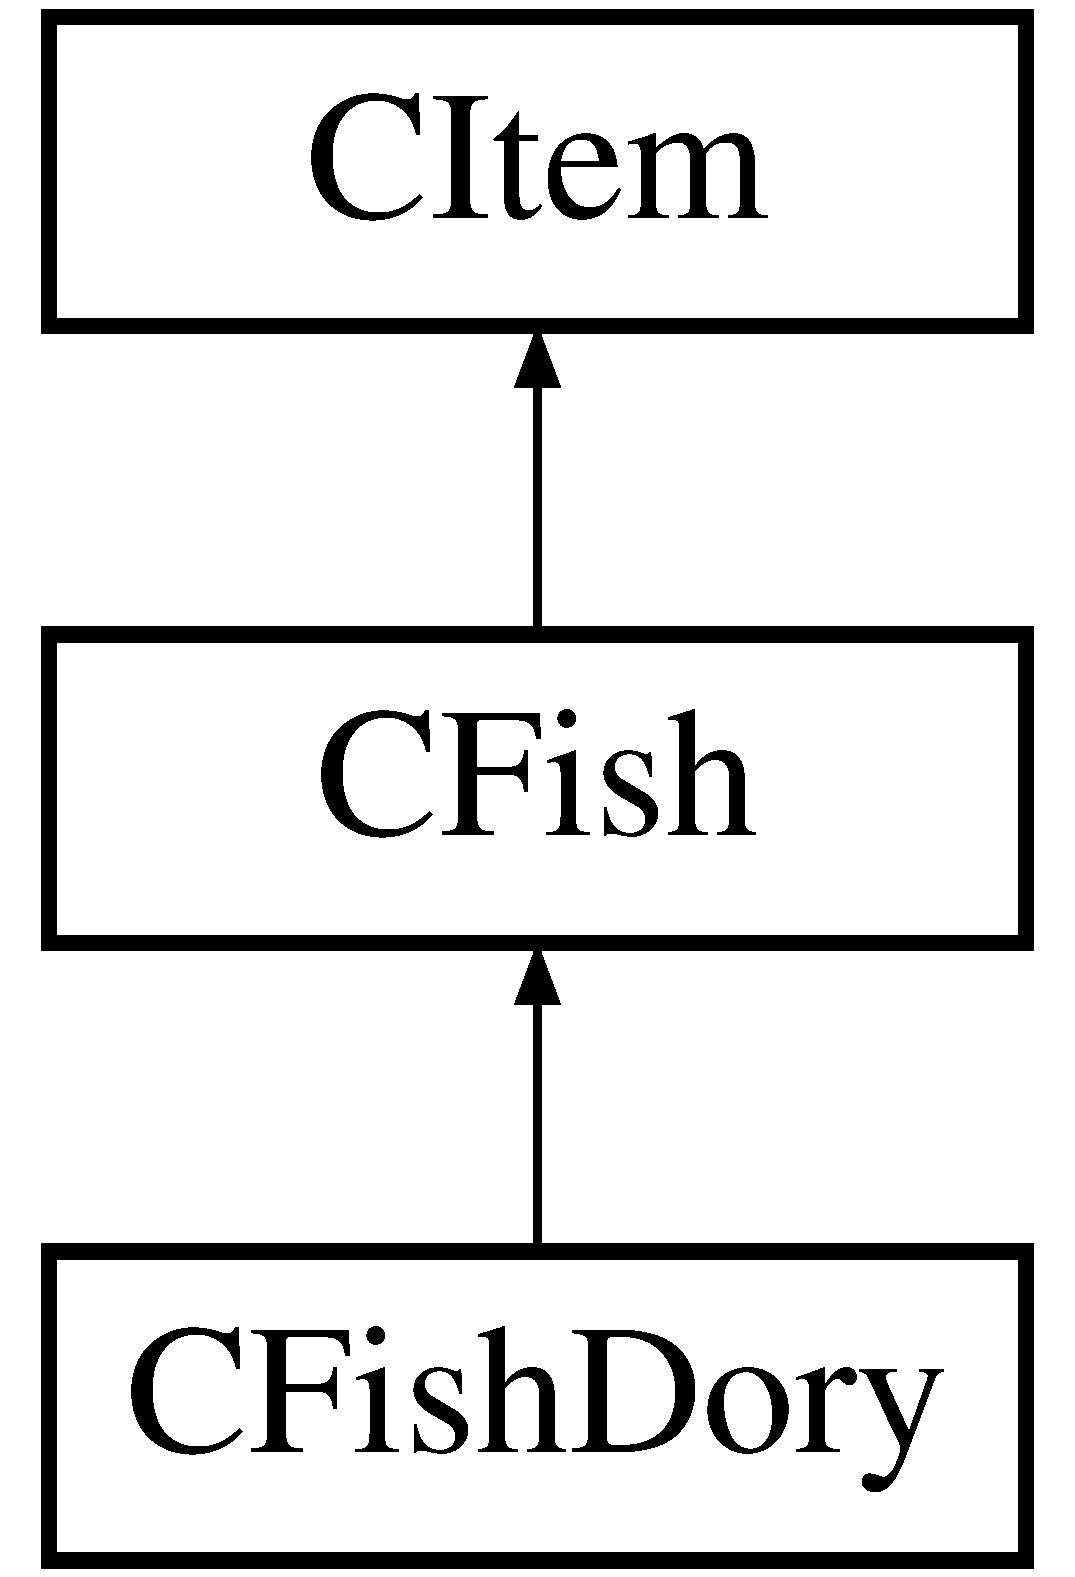
\includegraphics[height=3.000000cm]{class_c_fish_dory}
\end{center}
\end{figure}
\subsection*{Public Member Functions}
\begin{DoxyCompactItemize}
\item 
\mbox{\hyperlink{class_c_fish_dory_a7ed7364e99765e9424fc30e8de6124d9}{C\+Fish\+Dory}} (\mbox{\hyperlink{class_c_aquarium}{C\+Aquarium}} $\ast$aquarium)
\item 
\mbox{\Hypertarget{class_c_fish_dory_a4be4a33a09b36bbf4a5d5a9fa2130d99}\label{class_c_fish_dory_a4be4a33a09b36bbf4a5d5a9fa2130d99}} 
\mbox{\hyperlink{class_c_fish_dory_a4be4a33a09b36bbf4a5d5a9fa2130d99}{C\+Fish\+Dory}} ()=delete
\begin{DoxyCompactList}\small\item\em Default constructor (disabled) \end{DoxyCompactList}\item 
\mbox{\Hypertarget{class_c_fish_dory_a5db32b267a3553013bd9c15620a88b24}\label{class_c_fish_dory_a5db32b267a3553013bd9c15620a88b24}} 
\mbox{\hyperlink{class_c_fish_dory_a5db32b267a3553013bd9c15620a88b24}{C\+Fish\+Dory}} (const \mbox{\hyperlink{class_c_fish_dory}{C\+Fish\+Dory}} \&)=delete
\begin{DoxyCompactList}\small\item\em Copy constructor (disabled) \end{DoxyCompactList}\item 
virtual std\+::shared\+\_\+ptr$<$ \mbox{\hyperlink{classxmlnode_1_1_c_xml_node}{xmlnode\+::\+C\+Xml\+Node}} $>$ \mbox{\hyperlink{class_c_fish_dory_ac906b7f952cdbc52a72d1e87c9228ad9}{Xml\+Save}} (const std\+::shared\+\_\+ptr$<$ \mbox{\hyperlink{classxmlnode_1_1_c_xml_node}{xmlnode\+::\+C\+Xml\+Node}} $>$ \&node) override
\item 
virtual \mbox{\hyperlink{class_c_fish_dory_abe5cd45721286d8a67aacbe5e3cdc580}{$\sim$\+C\+Fish\+Dory}} ()
\end{DoxyCompactItemize}
\subsection*{Additional Inherited Members}


\subsection{Detailed Description}
Implements a Dory fish 

\subsection{Constructor \& Destructor Documentation}
\mbox{\Hypertarget{class_c_fish_dory_a7ed7364e99765e9424fc30e8de6124d9}\label{class_c_fish_dory_a7ed7364e99765e9424fc30e8de6124d9}} 
\index{C\+Fish\+Dory@{C\+Fish\+Dory}!C\+Fish\+Dory@{C\+Fish\+Dory}}
\index{C\+Fish\+Dory@{C\+Fish\+Dory}!C\+Fish\+Dory@{C\+Fish\+Dory}}
\subsubsection{\texorpdfstring{C\+Fish\+Dory()}{CFishDory()}}
{\footnotesize\ttfamily C\+Fish\+Dory\+::\+C\+Fish\+Dory (\begin{DoxyParamCaption}\item[{\mbox{\hyperlink{class_c_aquarium}{C\+Aquarium}} $\ast$}]{aquarium }\end{DoxyParamCaption})}

Constructor 
\begin{DoxyParams}{Parameters}
{\em aquarium} & The aquarium this is a member of \\
\hline
\end{DoxyParams}
\mbox{\Hypertarget{class_c_fish_dory_abe5cd45721286d8a67aacbe5e3cdc580}\label{class_c_fish_dory_abe5cd45721286d8a67aacbe5e3cdc580}} 
\index{C\+Fish\+Dory@{C\+Fish\+Dory}!````~C\+Fish\+Dory@{$\sim$\+C\+Fish\+Dory}}
\index{````~C\+Fish\+Dory@{$\sim$\+C\+Fish\+Dory}!C\+Fish\+Dory@{C\+Fish\+Dory}}
\subsubsection{\texorpdfstring{$\sim$\+C\+Fish\+Dory()}{~CFishDory()}}
{\footnotesize\ttfamily C\+Fish\+Dory\+::$\sim$\+C\+Fish\+Dory (\begin{DoxyParamCaption}{ }\end{DoxyParamCaption})\hspace{0.3cm}{\ttfamily [virtual]}}

Destructor 

\subsection{Member Function Documentation}
\mbox{\Hypertarget{class_c_fish_dory_ac906b7f952cdbc52a72d1e87c9228ad9}\label{class_c_fish_dory_ac906b7f952cdbc52a72d1e87c9228ad9}} 
\index{C\+Fish\+Dory@{C\+Fish\+Dory}!Xml\+Save@{Xml\+Save}}
\index{Xml\+Save@{Xml\+Save}!C\+Fish\+Dory@{C\+Fish\+Dory}}
\subsubsection{\texorpdfstring{Xml\+Save()}{XmlSave()}}
{\footnotesize\ttfamily std\+::shared\+\_\+ptr$<$ \mbox{\hyperlink{classxmlnode_1_1_c_xml_node}{xmlnode\+::\+C\+Xml\+Node}} $>$ C\+Fish\+Dory\+::\+Xml\+Save (\begin{DoxyParamCaption}\item[{const std\+::shared\+\_\+ptr$<$ \mbox{\hyperlink{classxmlnode_1_1_c_xml_node}{xmlnode\+::\+C\+Xml\+Node}} $>$ \&}]{node }\end{DoxyParamCaption})\hspace{0.3cm}{\ttfamily [override]}, {\ttfamily [virtual]}}

Save this item to an X\+ML node 
\begin{DoxyParams}{Parameters}
{\em node} & The node we are going to be a child of \\
\hline
\end{DoxyParams}


Reimplemented from \mbox{\hyperlink{class_c_fish_abfc997d2d755be8f94069c57e75a854b}{C\+Fish}}.



The documentation for this class was generated from the following files\+:\begin{DoxyCompactItemize}
\item 
Fish\+Dory.\+h\item 
\mbox{\hyperlink{_fish_dory_8cpp}{Fish\+Dory.\+cpp}}\end{DoxyCompactItemize}

\hypertarget{class_c_fish_karp}{}\section{C\+Fish\+Karp Class Reference}
\label{class_c_fish_karp}\index{C\+Fish\+Karp@{C\+Fish\+Karp}}


{\ttfamily \#include $<$Fish\+Karp.\+h$>$}

Inheritance diagram for C\+Fish\+Karp\+:\begin{figure}[H]
\begin{center}
\leavevmode
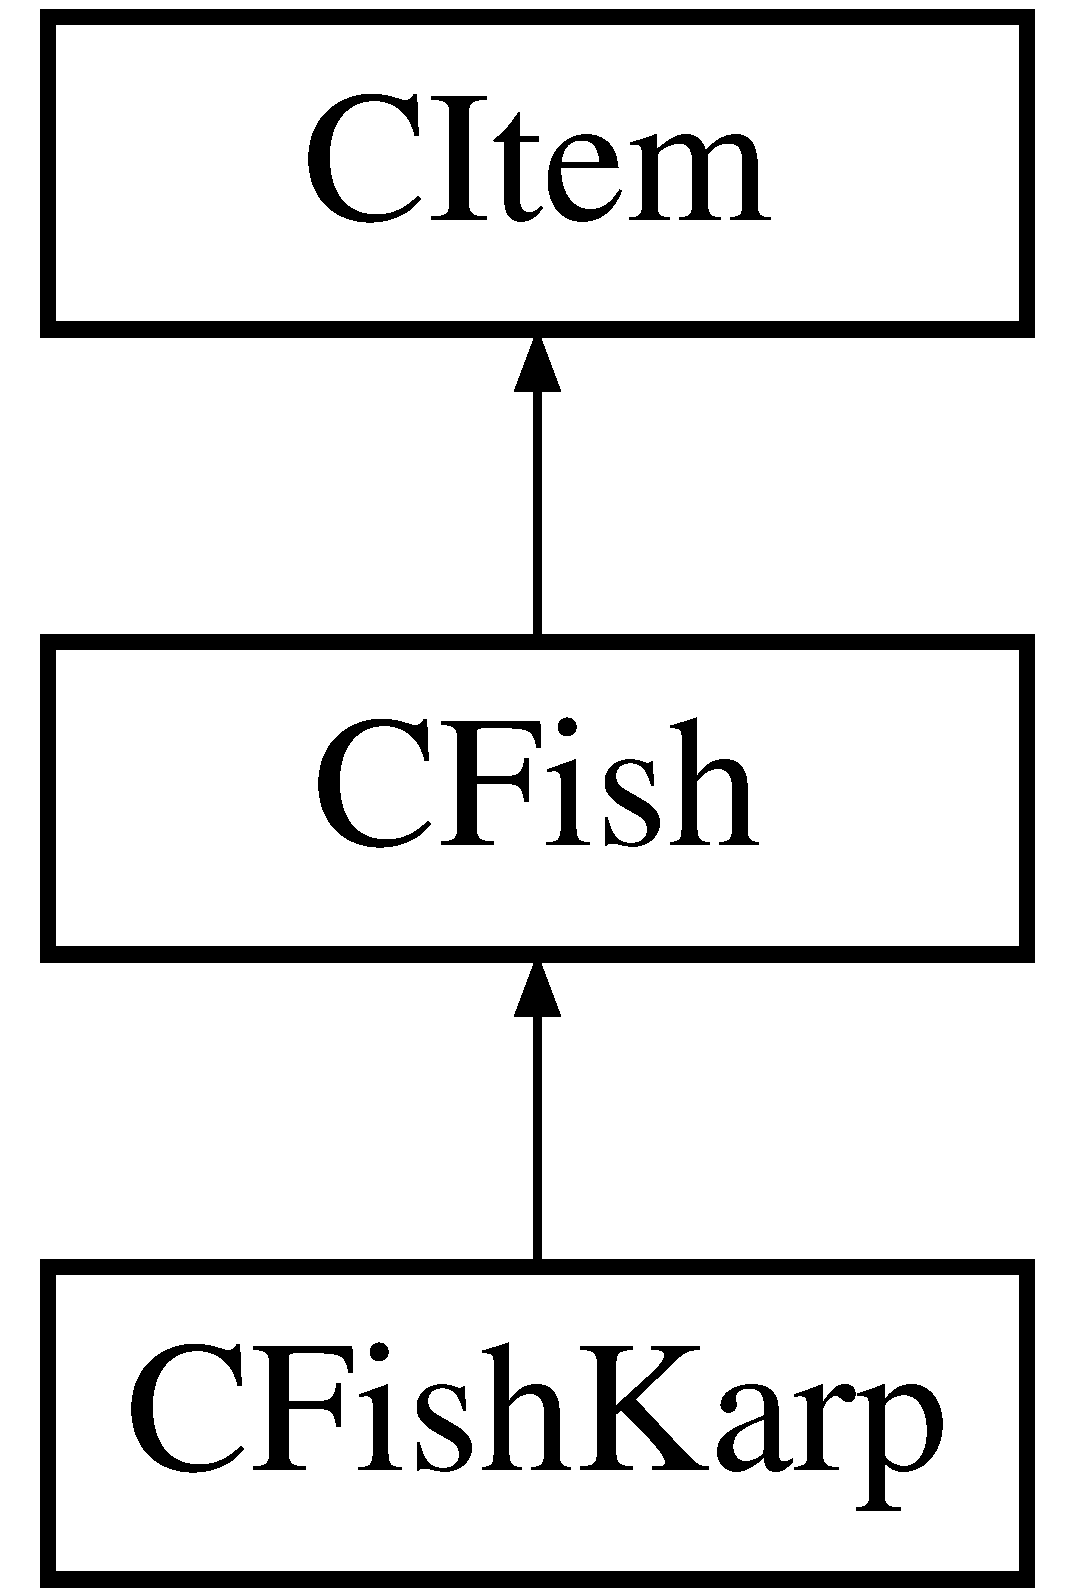
\includegraphics[height=3.000000cm]{class_c_fish_karp}
\end{center}
\end{figure}
\subsection*{Public Member Functions}
\begin{DoxyCompactItemize}
\item 
\mbox{\hyperlink{class_c_fish_karp_a6852207eec4ed8fa617409cb2dff4681}{C\+Fish\+Karp}} (\mbox{\hyperlink{class_c_aquarium}{C\+Aquarium}} $\ast$aquarium)
\item 
\mbox{\Hypertarget{class_c_fish_karp_a23fe85d81e982ce2c4346ed58b2bb60e}\label{class_c_fish_karp_a23fe85d81e982ce2c4346ed58b2bb60e}} 
\mbox{\hyperlink{class_c_fish_karp_a23fe85d81e982ce2c4346ed58b2bb60e}{C\+Fish\+Karp}} ()=delete
\begin{DoxyCompactList}\small\item\em Default constructor (disabled) \end{DoxyCompactList}\item 
\mbox{\Hypertarget{class_c_fish_karp_a252e6c2d527dc7697ffa21514742c2e2}\label{class_c_fish_karp_a252e6c2d527dc7697ffa21514742c2e2}} 
\mbox{\hyperlink{class_c_fish_karp_a252e6c2d527dc7697ffa21514742c2e2}{C\+Fish\+Karp}} (const \mbox{\hyperlink{class_c_fish_karp}{C\+Fish\+Karp}} \&)=delete
\begin{DoxyCompactList}\small\item\em Copy constructor (disabled) \end{DoxyCompactList}\item 
virtual std\+::shared\+\_\+ptr$<$ \mbox{\hyperlink{classxmlnode_1_1_c_xml_node}{xmlnode\+::\+C\+Xml\+Node}} $>$ \mbox{\hyperlink{class_c_fish_karp_a182d8cce606be73a981bd140aca64ba8}{Xml\+Save}} (const std\+::shared\+\_\+ptr$<$ \mbox{\hyperlink{classxmlnode_1_1_c_xml_node}{xmlnode\+::\+C\+Xml\+Node}} $>$ \&node) override
\item 
virtual \mbox{\hyperlink{class_c_fish_karp_a8e89f8df98a055864179326657919755}{$\sim$\+C\+Fish\+Karp}} ()
\item 
virtual void \mbox{\hyperlink{class_c_fish_karp_ad16715dc334ff9bbb96906463c67efe1}{Set\+Location}} (double x, double y)
\end{DoxyCompactItemize}
\subsection*{Additional Inherited Members}


\subsection{Detailed Description}
Implements a Karp fish 

\subsection{Constructor \& Destructor Documentation}
\mbox{\Hypertarget{class_c_fish_karp_a6852207eec4ed8fa617409cb2dff4681}\label{class_c_fish_karp_a6852207eec4ed8fa617409cb2dff4681}} 
\index{C\+Fish\+Karp@{C\+Fish\+Karp}!C\+Fish\+Karp@{C\+Fish\+Karp}}
\index{C\+Fish\+Karp@{C\+Fish\+Karp}!C\+Fish\+Karp@{C\+Fish\+Karp}}
\subsubsection{\texorpdfstring{C\+Fish\+Karp()}{CFishKarp()}}
{\footnotesize\ttfamily C\+Fish\+Karp\+::\+C\+Fish\+Karp (\begin{DoxyParamCaption}\item[{\mbox{\hyperlink{class_c_aquarium}{C\+Aquarium}} $\ast$}]{aquarium }\end{DoxyParamCaption})}

Constructor 
\begin{DoxyParams}{Parameters}
{\em aquarium} & The aquarium this is a member of \\
\hline
\end{DoxyParams}
\mbox{\Hypertarget{class_c_fish_karp_a8e89f8df98a055864179326657919755}\label{class_c_fish_karp_a8e89f8df98a055864179326657919755}} 
\index{C\+Fish\+Karp@{C\+Fish\+Karp}!````~C\+Fish\+Karp@{$\sim$\+C\+Fish\+Karp}}
\index{````~C\+Fish\+Karp@{$\sim$\+C\+Fish\+Karp}!C\+Fish\+Karp@{C\+Fish\+Karp}}
\subsubsection{\texorpdfstring{$\sim$\+C\+Fish\+Karp()}{~CFishKarp()}}
{\footnotesize\ttfamily C\+Fish\+Karp\+::$\sim$\+C\+Fish\+Karp (\begin{DoxyParamCaption}{ }\end{DoxyParamCaption})\hspace{0.3cm}{\ttfamily [virtual]}}

Destructor 

\subsection{Member Function Documentation}
\mbox{\Hypertarget{class_c_fish_karp_ad16715dc334ff9bbb96906463c67efe1}\label{class_c_fish_karp_ad16715dc334ff9bbb96906463c67efe1}} 
\index{C\+Fish\+Karp@{C\+Fish\+Karp}!Set\+Location@{Set\+Location}}
\index{Set\+Location@{Set\+Location}!C\+Fish\+Karp@{C\+Fish\+Karp}}
\subsubsection{\texorpdfstring{Set\+Location()}{SetLocation()}}
{\footnotesize\ttfamily void C\+Fish\+Karp\+::\+Set\+Location (\begin{DoxyParamCaption}\item[{double}]{x,  }\item[{double}]{y }\end{DoxyParamCaption})\hspace{0.3cm}{\ttfamily [virtual]}}

Gets location of killer karp and kills 
\begin{DoxyParams}{Parameters}
{\em x} & \\
\hline
{\em y} & \\
\hline
\end{DoxyParams}
\mbox{\Hypertarget{class_c_fish_karp_a182d8cce606be73a981bd140aca64ba8}\label{class_c_fish_karp_a182d8cce606be73a981bd140aca64ba8}} 
\index{C\+Fish\+Karp@{C\+Fish\+Karp}!Xml\+Save@{Xml\+Save}}
\index{Xml\+Save@{Xml\+Save}!C\+Fish\+Karp@{C\+Fish\+Karp}}
\subsubsection{\texorpdfstring{Xml\+Save()}{XmlSave()}}
{\footnotesize\ttfamily std\+::shared\+\_\+ptr$<$ \mbox{\hyperlink{classxmlnode_1_1_c_xml_node}{xmlnode\+::\+C\+Xml\+Node}} $>$ C\+Fish\+Karp\+::\+Xml\+Save (\begin{DoxyParamCaption}\item[{const std\+::shared\+\_\+ptr$<$ \mbox{\hyperlink{classxmlnode_1_1_c_xml_node}{xmlnode\+::\+C\+Xml\+Node}} $>$ \&}]{node }\end{DoxyParamCaption})\hspace{0.3cm}{\ttfamily [override]}, {\ttfamily [virtual]}}

Save this item to an X\+ML node 
\begin{DoxyParams}{Parameters}
{\em node} & The node we are going to be a child of \\
\hline
\end{DoxyParams}


Reimplemented from \mbox{\hyperlink{class_c_fish_abfc997d2d755be8f94069c57e75a854b}{C\+Fish}}.



The documentation for this class was generated from the following files\+:\begin{DoxyCompactItemize}
\item 
\mbox{\hyperlink{_fish_karp_8h}{Fish\+Karp.\+h}}\item 
\mbox{\hyperlink{_fish_karp_8cpp}{Fish\+Karp.\+cpp}}\end{DoxyCompactItemize}

\hypertarget{class_c_fish_nemo}{}\section{C\+Fish\+Nemo Class Reference}
\label{class_c_fish_nemo}\index{C\+Fish\+Nemo@{C\+Fish\+Nemo}}


{\ttfamily \#include $<$Fish\+Nemo.\+h$>$}

Inheritance diagram for C\+Fish\+Nemo\+:\begin{figure}[H]
\begin{center}
\leavevmode
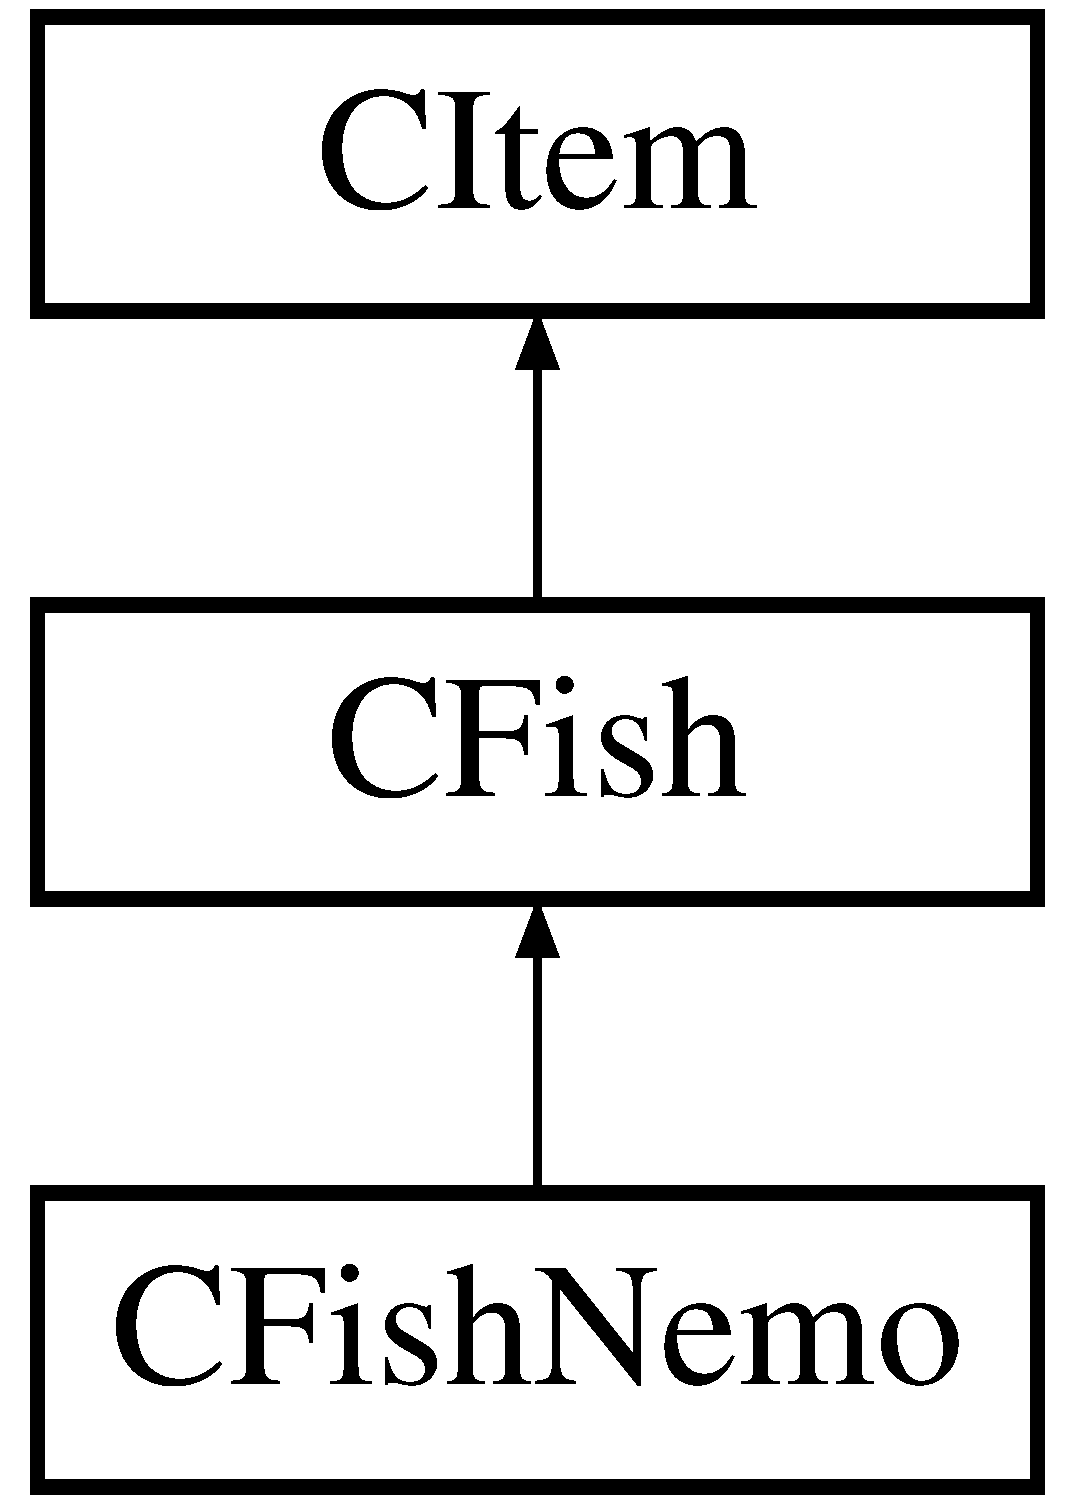
\includegraphics[height=3.000000cm]{class_c_fish_nemo}
\end{center}
\end{figure}
\subsection*{Public Member Functions}
\begin{DoxyCompactItemize}
\item 
\mbox{\hyperlink{class_c_fish_nemo_ab5cc8d119b0c9d8dc62a0e2b6f6e731d}{C\+Fish\+Nemo}} (\mbox{\hyperlink{class_c_aquarium}{C\+Aquarium}} $\ast$aquarium)
\item 
\mbox{\Hypertarget{class_c_fish_nemo_abb741271acb8aeb31fea93f5048d171e}\label{class_c_fish_nemo_abb741271acb8aeb31fea93f5048d171e}} 
\mbox{\hyperlink{class_c_fish_nemo_abb741271acb8aeb31fea93f5048d171e}{C\+Fish\+Nemo}} ()=delete
\begin{DoxyCompactList}\small\item\em Default constructor (disabled) \end{DoxyCompactList}\item 
\mbox{\Hypertarget{class_c_fish_nemo_a354e7fcb47bbf51c30c148c77dfbb59b}\label{class_c_fish_nemo_a354e7fcb47bbf51c30c148c77dfbb59b}} 
\mbox{\hyperlink{class_c_fish_nemo_a354e7fcb47bbf51c30c148c77dfbb59b}{C\+Fish\+Nemo}} (const \mbox{\hyperlink{class_c_fish_nemo}{C\+Fish\+Nemo}} \&)=delete
\begin{DoxyCompactList}\small\item\em Copy constructor (disabled) \end{DoxyCompactList}\item 
virtual std\+::shared\+\_\+ptr$<$ \mbox{\hyperlink{classxmlnode_1_1_c_xml_node}{xmlnode\+::\+C\+Xml\+Node}} $>$ \mbox{\hyperlink{class_c_fish_nemo_ae9fd9446cd4852c9d9a78831bec0f32f}{Xml\+Save}} (const std\+::shared\+\_\+ptr$<$ \mbox{\hyperlink{classxmlnode_1_1_c_xml_node}{xmlnode\+::\+C\+Xml\+Node}} $>$ \&node) override
\item 
virtual \mbox{\hyperlink{class_c_fish_nemo_ac37da91b4738144d3b47674450861b26}{$\sim$\+C\+Fish\+Nemo}} ()
\end{DoxyCompactItemize}
\subsection*{Additional Inherited Members}


\subsection{Detailed Description}
Implements a Nemo fish 

\subsection{Constructor \& Destructor Documentation}
\mbox{\Hypertarget{class_c_fish_nemo_ab5cc8d119b0c9d8dc62a0e2b6f6e731d}\label{class_c_fish_nemo_ab5cc8d119b0c9d8dc62a0e2b6f6e731d}} 
\index{C\+Fish\+Nemo@{C\+Fish\+Nemo}!C\+Fish\+Nemo@{C\+Fish\+Nemo}}
\index{C\+Fish\+Nemo@{C\+Fish\+Nemo}!C\+Fish\+Nemo@{C\+Fish\+Nemo}}
\subsubsection{\texorpdfstring{C\+Fish\+Nemo()}{CFishNemo()}}
{\footnotesize\ttfamily C\+Fish\+Nemo\+::\+C\+Fish\+Nemo (\begin{DoxyParamCaption}\item[{\mbox{\hyperlink{class_c_aquarium}{C\+Aquarium}} $\ast$}]{aquarium }\end{DoxyParamCaption})}

Constructor 
\begin{DoxyParams}{Parameters}
{\em aquarium} & The aquarium this is a member of \\
\hline
\end{DoxyParams}
\mbox{\Hypertarget{class_c_fish_nemo_ac37da91b4738144d3b47674450861b26}\label{class_c_fish_nemo_ac37da91b4738144d3b47674450861b26}} 
\index{C\+Fish\+Nemo@{C\+Fish\+Nemo}!````~C\+Fish\+Nemo@{$\sim$\+C\+Fish\+Nemo}}
\index{````~C\+Fish\+Nemo@{$\sim$\+C\+Fish\+Nemo}!C\+Fish\+Nemo@{C\+Fish\+Nemo}}
\subsubsection{\texorpdfstring{$\sim$\+C\+Fish\+Nemo()}{~CFishNemo()}}
{\footnotesize\ttfamily C\+Fish\+Nemo\+::$\sim$\+C\+Fish\+Nemo (\begin{DoxyParamCaption}{ }\end{DoxyParamCaption})\hspace{0.3cm}{\ttfamily [virtual]}}

Destructor 

\subsection{Member Function Documentation}
\mbox{\Hypertarget{class_c_fish_nemo_ae9fd9446cd4852c9d9a78831bec0f32f}\label{class_c_fish_nemo_ae9fd9446cd4852c9d9a78831bec0f32f}} 
\index{C\+Fish\+Nemo@{C\+Fish\+Nemo}!Xml\+Save@{Xml\+Save}}
\index{Xml\+Save@{Xml\+Save}!C\+Fish\+Nemo@{C\+Fish\+Nemo}}
\subsubsection{\texorpdfstring{Xml\+Save()}{XmlSave()}}
{\footnotesize\ttfamily std\+::shared\+\_\+ptr$<$ \mbox{\hyperlink{classxmlnode_1_1_c_xml_node}{xmlnode\+::\+C\+Xml\+Node}} $>$ C\+Fish\+Nemo\+::\+Xml\+Save (\begin{DoxyParamCaption}\item[{const std\+::shared\+\_\+ptr$<$ \mbox{\hyperlink{classxmlnode_1_1_c_xml_node}{xmlnode\+::\+C\+Xml\+Node}} $>$ \&}]{node }\end{DoxyParamCaption})\hspace{0.3cm}{\ttfamily [override]}, {\ttfamily [virtual]}}

Save this item to an X\+ML node 
\begin{DoxyParams}{Parameters}
{\em node} & The node we are going to be a child of \\
\hline
\end{DoxyParams}


Reimplemented from \mbox{\hyperlink{class_c_fish_abfc997d2d755be8f94069c57e75a854b}{C\+Fish}}.



The documentation for this class was generated from the following files\+:\begin{DoxyCompactItemize}
\item 
\mbox{\hyperlink{_fish_nemo_8h}{Fish\+Nemo.\+h}}\item 
\mbox{\hyperlink{_fish_nemo_8cpp}{Fish\+Nemo.\+cpp}}\end{DoxyCompactItemize}

\hypertarget{classxmlnode_1_1_c_xml_node_1_1_children}{}\section{xmlnode\+:\+:C\+Xml\+Node\+:\+:Children Class Reference}
\label{classxmlnode_1_1_c_xml_node_1_1_children}\index{xmlnode\+::\+C\+Xml\+Node\+::\+Children@{xmlnode\+::\+C\+Xml\+Node\+::\+Children}}


Representation of children to support iteration.  




{\ttfamily \#include $<$Xml\+Node.\+h$>$}

\subsection*{Public Member Functions}
\begin{DoxyCompactItemize}
\item 
\mbox{\hyperlink{classxmlnode_1_1_c_xml_node_1_1_iterator}{Iterator}} \mbox{\hyperlink{classxmlnode_1_1_c_xml_node_1_1_children_a8f0cac16fdda64bbf10cb08eba606dd1}{begin}} ()
\begin{DoxyCompactList}\small\item\em Get the beginning of the child node collection. \end{DoxyCompactList}\item 
\mbox{\hyperlink{classxmlnode_1_1_c_xml_node_1_1_iterator}{Iterator}} \mbox{\hyperlink{classxmlnode_1_1_c_xml_node_1_1_children_a3fe6fb9e62c63d6a9ea46653608d42e8}{end}} ()
\begin{DoxyCompactList}\small\item\em Get the end of the child node collection. \end{DoxyCompactList}\end{DoxyCompactItemize}
\subsection*{Friends}
\begin{DoxyCompactItemize}
\item 
\mbox{\Hypertarget{classxmlnode_1_1_c_xml_node_1_1_children_a9830fc407400559db7e7783cc10a9394}\label{classxmlnode_1_1_c_xml_node_1_1_children_a9830fc407400559db7e7783cc10a9394}} 
class \mbox{\hyperlink{classxmlnode_1_1_c_xml_node_1_1_children_a9830fc407400559db7e7783cc10a9394}{Iterator}}
\begin{DoxyCompactList}\small\item\em Friend class. \end{DoxyCompactList}\item 
\mbox{\Hypertarget{classxmlnode_1_1_c_xml_node_1_1_children_a770307dc9d4e2e7005bcf200bae3066a}\label{classxmlnode_1_1_c_xml_node_1_1_children_a770307dc9d4e2e7005bcf200bae3066a}} 
class \mbox{\hyperlink{classxmlnode_1_1_c_xml_node_1_1_children_a770307dc9d4e2e7005bcf200bae3066a}{C\+Xml\+Node}}
\begin{DoxyCompactList}\small\item\em Friend class. \end{DoxyCompactList}\end{DoxyCompactItemize}


\subsection{Detailed Description}
Representation of children to support iteration. 

\subsection{Member Function Documentation}
\mbox{\Hypertarget{classxmlnode_1_1_c_xml_node_1_1_children_a8f0cac16fdda64bbf10cb08eba606dd1}\label{classxmlnode_1_1_c_xml_node_1_1_children_a8f0cac16fdda64bbf10cb08eba606dd1}} 
\index{xmlnode\+::\+C\+Xml\+Node\+::\+Children@{xmlnode\+::\+C\+Xml\+Node\+::\+Children}!begin@{begin}}
\index{begin@{begin}!xmlnode\+::\+C\+Xml\+Node\+::\+Children@{xmlnode\+::\+C\+Xml\+Node\+::\+Children}}
\subsubsection{\texorpdfstring{begin()}{begin()}}
{\footnotesize\ttfamily \mbox{\hyperlink{classxmlnode_1_1_c_xml_node_1_1_iterator}{C\+Xml\+Node\+::\+Iterator}} C\+Xml\+Node\+::\+Children\+::begin (\begin{DoxyParamCaption}{ }\end{DoxyParamCaption})}



Get the beginning of the child node collection. 

\begin{DoxyReturn}{Returns}
\mbox{\hyperlink{classxmlnode_1_1_c_xml_node_1_1_iterator}{Iterator}} at beginning of collection. 
\end{DoxyReturn}
\mbox{\Hypertarget{classxmlnode_1_1_c_xml_node_1_1_children_a3fe6fb9e62c63d6a9ea46653608d42e8}\label{classxmlnode_1_1_c_xml_node_1_1_children_a3fe6fb9e62c63d6a9ea46653608d42e8}} 
\index{xmlnode\+::\+C\+Xml\+Node\+::\+Children@{xmlnode\+::\+C\+Xml\+Node\+::\+Children}!end@{end}}
\index{end@{end}!xmlnode\+::\+C\+Xml\+Node\+::\+Children@{xmlnode\+::\+C\+Xml\+Node\+::\+Children}}
\subsubsection{\texorpdfstring{end()}{end()}}
{\footnotesize\ttfamily \mbox{\hyperlink{classxmlnode_1_1_c_xml_node_1_1_iterator}{C\+Xml\+Node\+::\+Iterator}} C\+Xml\+Node\+::\+Children\+::end (\begin{DoxyParamCaption}{ }\end{DoxyParamCaption})}



Get the end of the child node collection. 

\begin{DoxyReturn}{Returns}
\mbox{\hyperlink{classxmlnode_1_1_c_xml_node_1_1_iterator}{Iterator}} at end of collection. 
\end{DoxyReturn}


The documentation for this class was generated from the following files\+:\begin{DoxyCompactItemize}
\item 
\mbox{\hyperlink{_xml_node_8h}{Xml\+Node.\+h}}\item 
\mbox{\hyperlink{_xml_node_8cpp}{Xml\+Node.\+cpp}}\end{DoxyCompactItemize}

\hypertarget{class_c_item}{}\section{C\+Item Class Reference}
\label{class_c_item}\index{C\+Item@{C\+Item}}


{\ttfamily \#include $<$Item.\+h$>$}

Inheritance diagram for C\+Item\+:\begin{figure}[H]
\begin{center}
\leavevmode
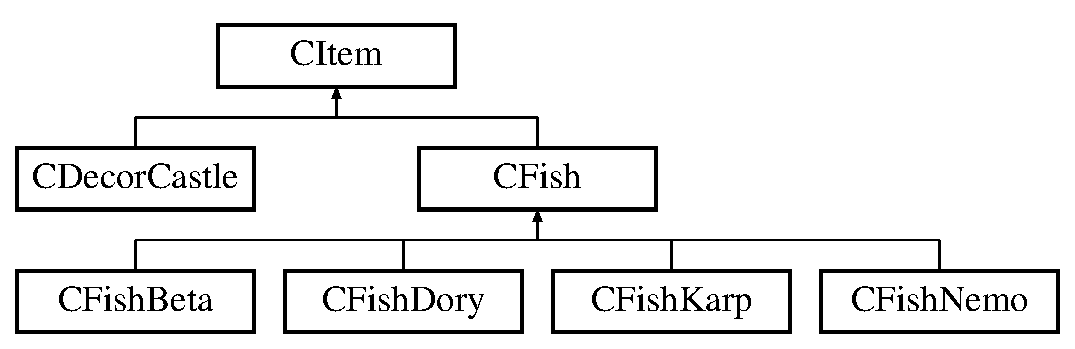
\includegraphics[height=2.000000cm]{class_c_item}
\end{center}
\end{figure}
\subsection*{Public Member Functions}
\begin{DoxyCompactItemize}
\item 
\mbox{\Hypertarget{class_c_item_ac2ea847c008cf8d1de92c870c8f8262f}\label{class_c_item_ac2ea847c008cf8d1de92c870c8f8262f}} 
\mbox{\hyperlink{class_c_item_ac2ea847c008cf8d1de92c870c8f8262f}{C\+Item}} ()=delete
\begin{DoxyCompactList}\small\item\em Default constructor (disabled) \end{DoxyCompactList}\item 
\mbox{\Hypertarget{class_c_item_a7d6042bbb9a571d2dc1d1f89016a97c8}\label{class_c_item_a7d6042bbb9a571d2dc1d1f89016a97c8}} 
\mbox{\hyperlink{class_c_item_a7d6042bbb9a571d2dc1d1f89016a97c8}{C\+Item}} (const \mbox{\hyperlink{class_c_item}{C\+Item}} \&)=delete
\begin{DoxyCompactList}\small\item\em Copy constructor (disabled) \end{DoxyCompactList}\item 
virtual \mbox{\hyperlink{class_c_item_a2487c6e822ed0e850544f1745b43f584}{$\sim$\+C\+Item}} ()
\item 
virtual void \mbox{\hyperlink{class_c_item_a7ef8448d0c4bc53d0f1943a4dc817f6f}{Draw}} (Gdiplus\+::\+Graphics $\ast$graphics)=0
\item 
double \mbox{\hyperlink{class_c_item_a394d38a058fc53f0e958ca52248560c8}{GetX}} () const
\item 
double \mbox{\hyperlink{class_c_item_ac0fe6be80f8ef19854d7f41b4803f658}{GetY}} () const
\item 
void \mbox{\hyperlink{class_c_item_a9c194f3f08e515853600cecca3e6d319}{Set\+Location}} (double x, double y)
\end{DoxyCompactItemize}
\subsection*{Protected Member Functions}
\begin{DoxyCompactItemize}
\item 
\mbox{\hyperlink{class_c_item_a665b3fa4628b43e69b1d7f2b9529882b}{C\+Item}} (\mbox{\hyperlink{class_c_aquarium}{C\+Aquarium}} $\ast$aquarium)
\end{DoxyCompactItemize}


\subsection{Detailed Description}
Instantiation of \mbox{\hyperlink{class_c_item}{C\+Item}} class. Responsible for detecting item movement to pull from. 

\subsection{Constructor \& Destructor Documentation}
\mbox{\Hypertarget{class_c_item_a2487c6e822ed0e850544f1745b43f584}\label{class_c_item_a2487c6e822ed0e850544f1745b43f584}} 
\index{C\+Item@{C\+Item}!````~C\+Item@{$\sim$\+C\+Item}}
\index{````~C\+Item@{$\sim$\+C\+Item}!C\+Item@{C\+Item}}
\subsubsection{\texorpdfstring{$\sim$\+C\+Item()}{~CItem()}}
{\footnotesize\ttfamily C\+Item\+::$\sim$\+C\+Item (\begin{DoxyParamCaption}{ }\end{DoxyParamCaption})\hspace{0.3cm}{\ttfamily [virtual]}}

Destructor \mbox{\Hypertarget{class_c_item_a665b3fa4628b43e69b1d7f2b9529882b}\label{class_c_item_a665b3fa4628b43e69b1d7f2b9529882b}} 
\index{C\+Item@{C\+Item}!C\+Item@{C\+Item}}
\index{C\+Item@{C\+Item}!C\+Item@{C\+Item}}
\subsubsection{\texorpdfstring{C\+Item()}{CItem()}}
{\footnotesize\ttfamily C\+Item\+::\+C\+Item (\begin{DoxyParamCaption}\item[{\mbox{\hyperlink{class_c_aquarium}{C\+Aquarium}} $\ast$}]{aquarium }\end{DoxyParamCaption})\hspace{0.3cm}{\ttfamily [protected]}}

Constructor 
\begin{DoxyParams}{Parameters}
{\em aquarium} & The aquarium that this item is a member of \\
\hline
\end{DoxyParams}


\subsection{Member Function Documentation}
\mbox{\Hypertarget{class_c_item_a7ef8448d0c4bc53d0f1943a4dc817f6f}\label{class_c_item_a7ef8448d0c4bc53d0f1943a4dc817f6f}} 
\index{C\+Item@{C\+Item}!Draw@{Draw}}
\index{Draw@{Draw}!C\+Item@{C\+Item}}
\subsubsection{\texorpdfstring{Draw()}{Draw()}}
{\footnotesize\ttfamily virtual void C\+Item\+::\+Draw (\begin{DoxyParamCaption}\item[{Gdiplus\+::\+Graphics $\ast$}]{graphics }\end{DoxyParamCaption})\hspace{0.3cm}{\ttfamily [pure virtual]}}

Draw this item 
\begin{DoxyParams}{Parameters}
{\em graphics} & Graphics device to draw on \\
\hline
\end{DoxyParams}


Implemented in \mbox{\hyperlink{class_c_fish_beta_ae2effbff7b98bb3cd6e1070d61d5366e}{C\+Fish\+Beta}}.

\mbox{\Hypertarget{class_c_item_a394d38a058fc53f0e958ca52248560c8}\label{class_c_item_a394d38a058fc53f0e958ca52248560c8}} 
\index{C\+Item@{C\+Item}!GetX@{GetX}}
\index{GetX@{GetX}!C\+Item@{C\+Item}}
\subsubsection{\texorpdfstring{Get\+X()}{GetX()}}
{\footnotesize\ttfamily double C\+Item\+::\+GetX (\begin{DoxyParamCaption}{ }\end{DoxyParamCaption}) const\hspace{0.3cm}{\ttfamily [inline]}}

The X location of the item \begin{DoxyReturn}{Returns}
X location in pixels 
\end{DoxyReturn}
\mbox{\Hypertarget{class_c_item_ac0fe6be80f8ef19854d7f41b4803f658}\label{class_c_item_ac0fe6be80f8ef19854d7f41b4803f658}} 
\index{C\+Item@{C\+Item}!GetY@{GetY}}
\index{GetY@{GetY}!C\+Item@{C\+Item}}
\subsubsection{\texorpdfstring{Get\+Y()}{GetY()}}
{\footnotesize\ttfamily double C\+Item\+::\+GetY (\begin{DoxyParamCaption}{ }\end{DoxyParamCaption}) const\hspace{0.3cm}{\ttfamily [inline]}}

The Y location of the item \begin{DoxyReturn}{Returns}
Y location in pixels 
\end{DoxyReturn}
\mbox{\Hypertarget{class_c_item_a9c194f3f08e515853600cecca3e6d319}\label{class_c_item_a9c194f3f08e515853600cecca3e6d319}} 
\index{C\+Item@{C\+Item}!Set\+Location@{Set\+Location}}
\index{Set\+Location@{Set\+Location}!C\+Item@{C\+Item}}
\subsubsection{\texorpdfstring{Set\+Location()}{SetLocation()}}
{\footnotesize\ttfamily void C\+Item\+::\+Set\+Location (\begin{DoxyParamCaption}\item[{double}]{x,  }\item[{double}]{y }\end{DoxyParamCaption})\hspace{0.3cm}{\ttfamily [inline]}}

Set the item location 
\begin{DoxyParams}{Parameters}
{\em x} & X location \\
\hline
{\em y} & Y location \\
\hline
\end{DoxyParams}


The documentation for this class was generated from the following files\+:\begin{DoxyCompactItemize}
\item 
\mbox{\hyperlink{_item_8h}{Item.\+h}}\item 
\mbox{\hyperlink{_item_8cpp}{Item.\+cpp}}\end{DoxyCompactItemize}

\hypertarget{class_c_main_frame}{}\section{C\+Main\+Frame Class Reference}
\label{class_c_main_frame}\index{C\+Main\+Frame@{C\+Main\+Frame}}
Inheritance diagram for C\+Main\+Frame\+:\begin{figure}[H]
\begin{center}
\leavevmode
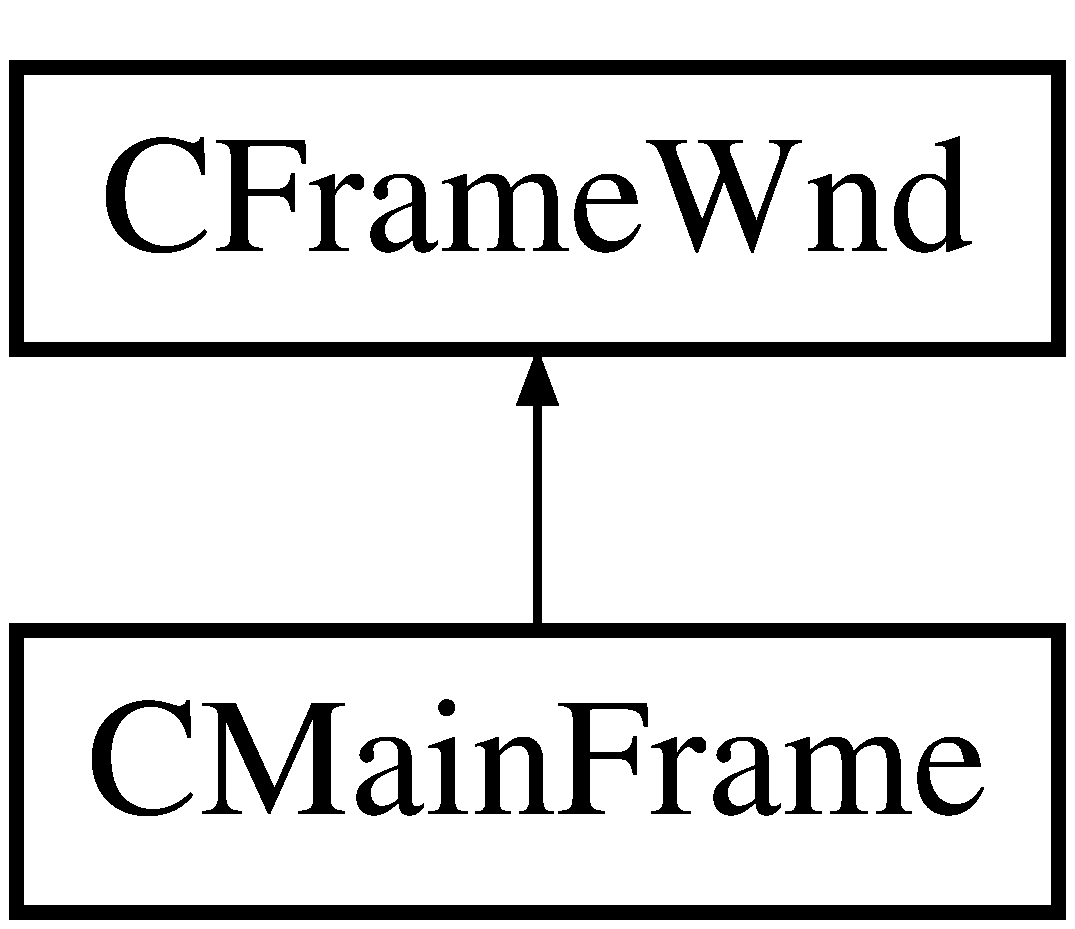
\includegraphics[height=2.000000cm]{class_c_main_frame}
\end{center}
\end{figure}
\subsection*{Public Member Functions}
\begin{DoxyCompactItemize}
\item 
virtual B\+O\+OL \mbox{\hyperlink{class_c_main_frame_a549bf677c955c2898c3c683321633c16}{Pre\+Create\+Window}} (C\+R\+E\+A\+T\+E\+S\+T\+R\+U\+CT \&cs)
\item 
virtual B\+O\+OL \mbox{\hyperlink{class_c_main_frame_ade959eb0bab719bf06bb9b18ee407101}{On\+Cmd\+Msg}} (U\+I\+NT n\+ID, int n\+Code, void $\ast$p\+Extra, A\+F\+X\+\_\+\+C\+M\+D\+H\+A\+N\+D\+L\+E\+R\+I\+N\+FO $\ast$p\+Handler\+Info)
\end{DoxyCompactItemize}
\subsection*{Protected Member Functions}
\begin{DoxyCompactItemize}
\item 
afx\+\_\+msg int \mbox{\hyperlink{class_c_main_frame_a48666466fd37412fcaeff75c3b12e0ed}{On\+Create}} (L\+P\+C\+R\+E\+A\+T\+E\+S\+T\+R\+U\+CT lp\+Create\+Struct)
\item 
afx\+\_\+msg void \mbox{\hyperlink{class_c_main_frame_adc353a3d1fc497fbc009b6d9e6914a82}{On\+Set\+Focus}} (C\+Wnd $\ast$p\+Old\+Wnd)
\end{DoxyCompactItemize}
\subsection*{Protected Attributes}
\begin{DoxyCompactItemize}
\item 
\mbox{\Hypertarget{class_c_main_frame_a73024d794dce2fe918f6b117371c25fc}\label{class_c_main_frame_a73024d794dce2fe918f6b117371c25fc}} 
C\+Tool\+Bar {\bfseries m\+\_\+wnd\+Tool\+Bar}
\item 
\mbox{\Hypertarget{class_c_main_frame_ac01bafc03aee69cf982e6f029b4db6b0}\label{class_c_main_frame_ac01bafc03aee69cf982e6f029b4db6b0}} 
C\+Status\+Bar {\bfseries m\+\_\+wnd\+Status\+Bar}
\item 
\mbox{\Hypertarget{class_c_main_frame_a7c3af9327c496f8c807d578f7a4ef4c5}\label{class_c_main_frame_a7c3af9327c496f8c807d578f7a4ef4c5}} 
\mbox{\hyperlink{class_c_child_view}{C\+Child\+View}} {\bfseries m\+\_\+wnd\+View}
\end{DoxyCompactItemize}


\subsection{Member Function Documentation}
\mbox{\Hypertarget{class_c_main_frame_ade959eb0bab719bf06bb9b18ee407101}\label{class_c_main_frame_ade959eb0bab719bf06bb9b18ee407101}} 
\index{C\+Main\+Frame@{C\+Main\+Frame}!On\+Cmd\+Msg@{On\+Cmd\+Msg}}
\index{On\+Cmd\+Msg@{On\+Cmd\+Msg}!C\+Main\+Frame@{C\+Main\+Frame}}
\subsubsection{\texorpdfstring{On\+Cmd\+Msg()}{OnCmdMsg()}}
{\footnotesize\ttfamily B\+O\+OL C\+Main\+Frame\+::\+On\+Cmd\+Msg (\begin{DoxyParamCaption}\item[{U\+I\+NT}]{n\+ID,  }\item[{int}]{n\+Code,  }\item[{void $\ast$}]{p\+Extra,  }\item[{A\+F\+X\+\_\+\+C\+M\+D\+H\+A\+N\+D\+L\+E\+R\+I\+N\+FO $\ast$}]{p\+Handler\+Info }\end{DoxyParamCaption})\hspace{0.3cm}{\ttfamily [virtual]}}

Checking for command messages 
\begin{DoxyParams}{Parameters}
{\em n\+ID} & \\
\hline
{\em n\+Code} & \\
\hline
{\em p\+Extra} & \\
\hline
{\em p\+Handler\+Info} & \\
\hline
\end{DoxyParams}
\begin{DoxyReturn}{Returns}

\end{DoxyReturn}
\mbox{\Hypertarget{class_c_main_frame_a48666466fd37412fcaeff75c3b12e0ed}\label{class_c_main_frame_a48666466fd37412fcaeff75c3b12e0ed}} 
\index{C\+Main\+Frame@{C\+Main\+Frame}!On\+Create@{On\+Create}}
\index{On\+Create@{On\+Create}!C\+Main\+Frame@{C\+Main\+Frame}}
\subsubsection{\texorpdfstring{On\+Create()}{OnCreate()}}
{\footnotesize\ttfamily int C\+Main\+Frame\+::\+On\+Create (\begin{DoxyParamCaption}\item[{L\+P\+C\+R\+E\+A\+T\+E\+S\+T\+R\+U\+CT}]{lp\+Create\+Struct }\end{DoxyParamCaption})\hspace{0.3cm}{\ttfamily [protected]}}

Creation of Mainframe window 
\begin{DoxyParams}{Parameters}
{\em lp\+Create\+Struct} & \\
\hline
\end{DoxyParams}
\begin{DoxyReturn}{Returns}

\end{DoxyReturn}
\mbox{\Hypertarget{class_c_main_frame_adc353a3d1fc497fbc009b6d9e6914a82}\label{class_c_main_frame_adc353a3d1fc497fbc009b6d9e6914a82}} 
\index{C\+Main\+Frame@{C\+Main\+Frame}!On\+Set\+Focus@{On\+Set\+Focus}}
\index{On\+Set\+Focus@{On\+Set\+Focus}!C\+Main\+Frame@{C\+Main\+Frame}}
\subsubsection{\texorpdfstring{On\+Set\+Focus()}{OnSetFocus()}}
{\footnotesize\ttfamily void C\+Main\+Frame\+::\+On\+Set\+Focus (\begin{DoxyParamCaption}\item[{C\+Wnd $\ast$}]{p\+Old\+Wnd }\end{DoxyParamCaption})\hspace{0.3cm}{\ttfamily [protected]}}

Setting the focus of the mainframe window \mbox{\hyperlink{class_c_main_frame}{C\+Main\+Frame}} message handlers 
\begin{DoxyParams}{Parameters}
{\em } & \\
\hline
\end{DoxyParams}
\mbox{\Hypertarget{class_c_main_frame_a549bf677c955c2898c3c683321633c16}\label{class_c_main_frame_a549bf677c955c2898c3c683321633c16}} 
\index{C\+Main\+Frame@{C\+Main\+Frame}!Pre\+Create\+Window@{Pre\+Create\+Window}}
\index{Pre\+Create\+Window@{Pre\+Create\+Window}!C\+Main\+Frame@{C\+Main\+Frame}}
\subsubsection{\texorpdfstring{Pre\+Create\+Window()}{PreCreateWindow()}}
{\footnotesize\ttfamily B\+O\+OL C\+Main\+Frame\+::\+Pre\+Create\+Window (\begin{DoxyParamCaption}\item[{C\+R\+E\+A\+T\+E\+S\+T\+R\+U\+CT \&}]{cs }\end{DoxyParamCaption})\hspace{0.3cm}{\ttfamily [virtual]}}

Pre\+Creation of Main\+Frame Window for Aquarium 
\begin{DoxyParams}{Parameters}
{\em cs} & \\
\hline
\end{DoxyParams}
\begin{DoxyReturn}{Returns}

\end{DoxyReturn}


The documentation for this class was generated from the following files\+:\begin{DoxyCompactItemize}
\item 
Main\+Frm.\+h\item 
Main\+Frm.\+cpp\end{DoxyCompactItemize}

\hypertarget{class_c_step2_app}{}\section{C\+Step2\+App Class Reference}
\label{class_c_step2_app}\index{C\+Step2\+App@{C\+Step2\+App}}
Inheritance diagram for C\+Step2\+App\+:\begin{figure}[H]
\begin{center}
\leavevmode
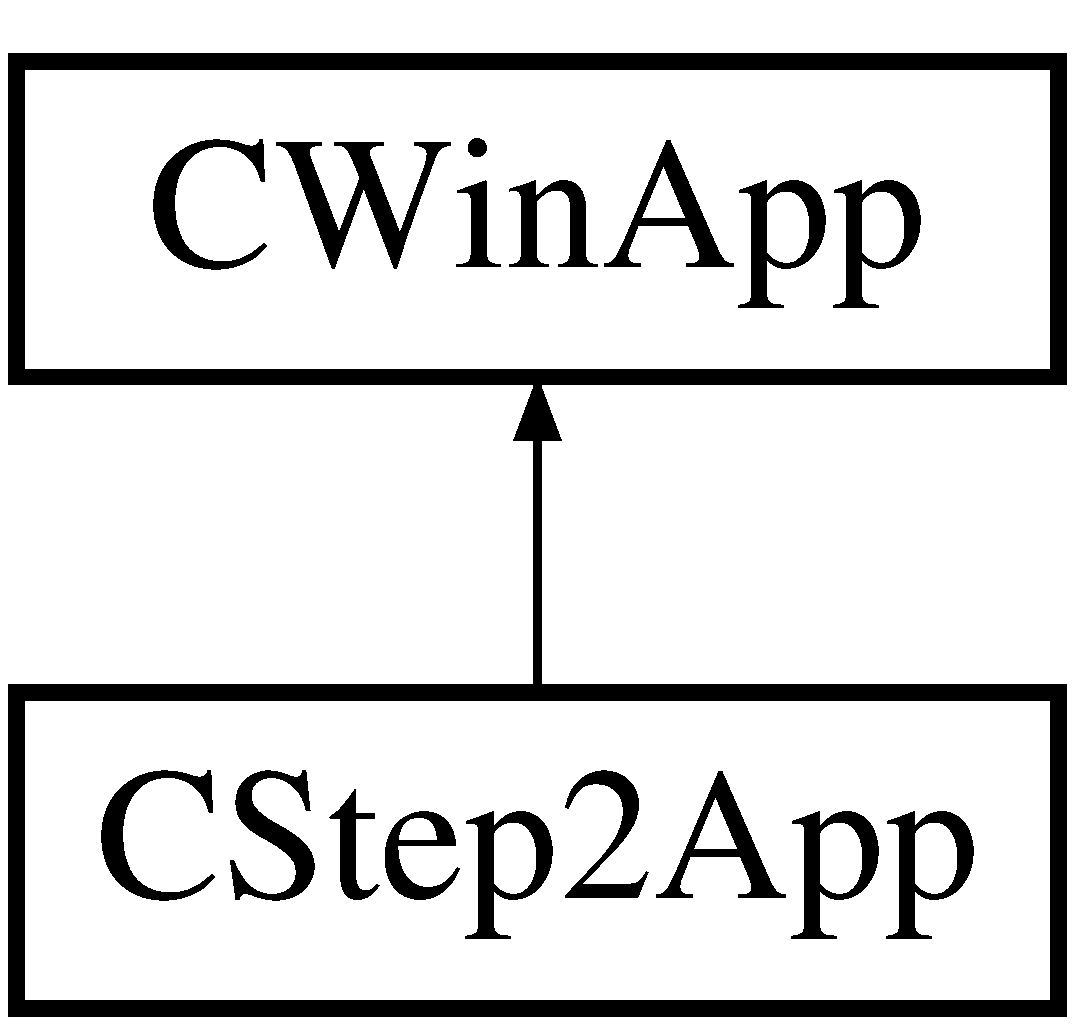
\includegraphics[height=2.000000cm]{class_c_step2_app}
\end{center}
\end{figure}
\subsection*{Public Member Functions}
\begin{DoxyCompactItemize}
\item 
\mbox{\Hypertarget{class_c_step2_app_a4152bf861e6e520eaa173c41a3d9f73d}\label{class_c_step2_app_a4152bf861e6e520eaa173c41a3d9f73d}} 
virtual B\+O\+OL {\bfseries Init\+Instance} ()
\item 
\mbox{\Hypertarget{class_c_step2_app_aad455705e63bb9ae0642be6ca2d2b684}\label{class_c_step2_app_aad455705e63bb9ae0642be6ca2d2b684}} 
virtual int {\bfseries Exit\+Instance} ()
\item 
\mbox{\Hypertarget{class_c_step2_app_a7407f02b1d0628458512c9f35ab2bb50}\label{class_c_step2_app_a7407f02b1d0628458512c9f35ab2bb50}} 
afx\+\_\+msg void {\bfseries On\+App\+About} ()
\end{DoxyCompactItemize}


The documentation for this class was generated from the following files\+:\begin{DoxyCompactItemize}
\item 
Step2.\+h\item 
Step2.\+cpp\end{DoxyCompactItemize}

\hypertarget{classxmlnode_1_1_c_xml_node}{}\section{xmlnode\+:\+:C\+Xml\+Node Class Reference}
\label{classxmlnode_1_1_c_xml_node}\index{xmlnode\+::\+C\+Xml\+Node@{xmlnode\+::\+C\+Xml\+Node}}


A wrapper for msxml nodes.  




{\ttfamily \#include $<$Xml\+Node.\+h$>$}

\subsection*{Classes}
\begin{DoxyCompactItemize}
\item 
class \mbox{\hyperlink{classxmlnode_1_1_c_xml_node_1_1_children}{Children}}
\begin{DoxyCompactList}\small\item\em Representation of children to support iteration. \end{DoxyCompactList}\item 
class \mbox{\hyperlink{classxmlnode_1_1_c_xml_node_1_1_exception}{Exception}}
\begin{DoxyCompactList}\small\item\em Exceptions for \mbox{\hyperlink{classxmlnode_1_1_c_xml_node}{C\+Xml\+Node}}. \end{DoxyCompactList}\item 
class \mbox{\hyperlink{classxmlnode_1_1_c_xml_node_1_1_iterator}{Iterator}}
\begin{DoxyCompactList}\small\item\em Support for iterating over the children of a node. \end{DoxyCompactList}\end{DoxyCompactItemize}
\subsection*{Public Member Functions}
\begin{DoxyCompactItemize}
\item 
\mbox{\hyperlink{classxmlnode_1_1_c_xml_node_a0f05b63e034bb5620609a2020c591d55}{C\+Xml\+Node}} ()
\begin{DoxyCompactList}\small\item\em Constructor. \end{DoxyCompactList}\item 
\mbox{\Hypertarget{classxmlnode_1_1_c_xml_node_ad3e072fa0d46c534c08f013405e051ae}\label{classxmlnode_1_1_c_xml_node_ad3e072fa0d46c534c08f013405e051ae}} 
virtual \mbox{\hyperlink{classxmlnode_1_1_c_xml_node_ad3e072fa0d46c534c08f013405e051ae}{$\sim$\+C\+Xml\+Node}} ()
\begin{DoxyCompactList}\small\item\em Destructor. \end{DoxyCompactList}\item 
void \mbox{\hyperlink{classxmlnode_1_1_c_xml_node_abfd7b791490e58aac7091b78e36bd24b}{Open}} (const std\+::wstring \&filename)
\begin{DoxyCompactList}\small\item\em Open a file as an X\+ML document. \end{DoxyCompactList}\item 
void \mbox{\hyperlink{classxmlnode_1_1_c_xml_node_a7f4a7dee5a7de490507b9d0ed78dbab7}{Create}} (const std\+::wstring \&rootname)
\begin{DoxyCompactList}\small\item\em Create an empty X\+ML document in this node. \end{DoxyCompactList}\item 
void \mbox{\hyperlink{classxmlnode_1_1_c_xml_node_a0f83eef381fe59726503e0fcb854661d}{Save}} (const std\+::wstring \&filename)
\begin{DoxyCompactList}\small\item\em Save X\+ML document to a file. \end{DoxyCompactList}\item 
std\+::wstring \mbox{\hyperlink{classxmlnode_1_1_c_xml_node_a700c3de386529eab05b185c38b17fd51}{Get\+X\+ML}} ()
\begin{DoxyCompactList}\small\item\em Obtain the created X\+ML as a string. \end{DoxyCompactList}\item 
std\+::wstring \mbox{\hyperlink{classxmlnode_1_1_c_xml_node_a84d2553bd71bde08ee2a65fb1eedf3a4}{Get\+Name}} () const
\begin{DoxyCompactList}\small\item\em The node name. \end{DoxyCompactList}\item 
D\+O\+M\+Node\+Type \mbox{\hyperlink{classxmlnode_1_1_c_xml_node_ac6a20070f4679d4b7e4e69b844692214}{Get\+Type}} () const
\begin{DoxyCompactList}\small\item\em The node type. \end{DoxyCompactList}\item 
std\+::wstring \mbox{\hyperlink{classxmlnode_1_1_c_xml_node_ac0593ce9fc62dd3e9777506c0c3a84bf}{Get\+Value}} () const
\begin{DoxyCompactList}\small\item\em Get the node value. \end{DoxyCompactList}\item 
int \mbox{\hyperlink{classxmlnode_1_1_c_xml_node_a436c9299f0a8d8ce57d42545cdc4c693}{Get\+Int\+Value}} () const
\begin{DoxyCompactList}\small\item\em Get the node value. \end{DoxyCompactList}\item 
double \mbox{\hyperlink{classxmlnode_1_1_c_xml_node_a8a2b2726257dc82a35fd2f7810c6ccf7}{Get\+Double\+Value}} () const
\begin{DoxyCompactList}\small\item\em Get the node value. \end{DoxyCompactList}\item 
std\+::shared\+\_\+ptr$<$ \mbox{\hyperlink{classxmlnode_1_1_c_xml_node}{C\+Xml\+Node}} $>$ \mbox{\hyperlink{classxmlnode_1_1_c_xml_node_aa571e6a48132a260420a077dde31168f}{Get\+Attribute}} (const std\+::wstring \&name)
\begin{DoxyCompactList}\small\item\em Get an attribute. \end{DoxyCompactList}\item 
std\+::wstring \mbox{\hyperlink{classxmlnode_1_1_c_xml_node_ac4b635b102a0ba6c0f64d047fd27f2a1}{Get\+Attribute\+Value}} (const std\+::wstring \&name, const std\+::wstring \&def)
\begin{DoxyCompactList}\small\item\em Get the value of an attribute. \end{DoxyCompactList}\item 
int \mbox{\hyperlink{classxmlnode_1_1_c_xml_node_a870618bd8862b8f3834613f469e56d25}{Get\+Attribute\+Int\+Value}} (const std\+::wstring \&name, int def)
\begin{DoxyCompactList}\small\item\em Get the value of an attribute. \end{DoxyCompactList}\item 
double \mbox{\hyperlink{classxmlnode_1_1_c_xml_node_a69fcfbe75f19450db6fe72908ce7c52e}{Get\+Attribute\+Double\+Value}} (const std\+::wstring \&name, double def)
\begin{DoxyCompactList}\small\item\em Get the value of an attribute. \end{DoxyCompactList}\item 
void \mbox{\hyperlink{classxmlnode_1_1_c_xml_node_ac2543c8908d29642f70c9ce437475bf1}{Set\+Attribute}} (const std\+::wstring \&name, const std\+::wstring \&val)
\begin{DoxyCompactList}\small\item\em Set an attribute on this node. \end{DoxyCompactList}\item 
void \mbox{\hyperlink{classxmlnode_1_1_c_xml_node_a6771d1de541ffefcf8a4fcd809b12b62}{Set\+Attribute}} (const std\+::wstring \&name, int val)
\begin{DoxyCompactList}\small\item\em Set an attribute on this node. \end{DoxyCompactList}\item 
void \mbox{\hyperlink{classxmlnode_1_1_c_xml_node_a1bfd97eb8de5e6f769b5ed29039b91ea}{Set\+Attribute}} (const std\+::wstring \&name, double val)
\begin{DoxyCompactList}\small\item\em Set an attribute on this node. \end{DoxyCompactList}\item 
std\+::shared\+\_\+ptr$<$ \mbox{\hyperlink{classxmlnode_1_1_c_xml_node}{C\+Xml\+Node}} $>$ \mbox{\hyperlink{classxmlnode_1_1_c_xml_node_ac5700bda1faebcbe5bb042e043ea60be}{Get\+Child}} (int n)
\begin{DoxyCompactList}\small\item\em Get a child node of this node by index. \end{DoxyCompactList}\item 
\mbox{\hyperlink{classxmlnode_1_1_c_xml_node_1_1_children}{Children}} \mbox{\hyperlink{classxmlnode_1_1_c_xml_node_a03f86570ca40d4cc09c3e1841939a9d0}{Get\+Children}} ()
\begin{DoxyCompactList}\small\item\em Get the children of this node. \end{DoxyCompactList}\item 
int \mbox{\hyperlink{classxmlnode_1_1_c_xml_node_ab455bd55e7f3dbd550e81d7fe293d146}{Get\+Num\+Children}} ()
\begin{DoxyCompactList}\small\item\em Number of children of this node. \end{DoxyCompactList}\item 
std\+::shared\+\_\+ptr$<$ \mbox{\hyperlink{classxmlnode_1_1_c_xml_node}{C\+Xml\+Node}} $>$ \mbox{\hyperlink{classxmlnode_1_1_c_xml_node_a7227a654358ffb87a2a57c165dee509c}{Add\+Child}} (const std\+::wstring \&name)
\begin{DoxyCompactList}\small\item\em Add a child node to this node. \end{DoxyCompactList}\end{DoxyCompactItemize}
\subsection*{Static Public Member Functions}
\begin{DoxyCompactItemize}
\item 
static std\+::shared\+\_\+ptr$<$ \mbox{\hyperlink{classxmlnode_1_1_c_xml_node}{C\+Xml\+Node}} $>$ \mbox{\hyperlink{classxmlnode_1_1_c_xml_node_ad71ff87937ae943a9c11f5891d53d93b}{Open\+Document}} (const std\+::wstring \&filename)
\begin{DoxyCompactList}\small\item\em Open an X\+ML document and return the document root node. \end{DoxyCompactList}\item 
static std\+::shared\+\_\+ptr$<$ \mbox{\hyperlink{classxmlnode_1_1_c_xml_node}{C\+Xml\+Node}} $>$ \mbox{\hyperlink{classxmlnode_1_1_c_xml_node_ae50a4482c4ea73492001f91788945bb1}{Create\+Document}} (const std\+::wstring \&rootname)
\begin{DoxyCompactList}\small\item\em Create an empty X\+ML document and return the document root node. \end{DoxyCompactList}\end{DoxyCompactItemize}


\subsection{Detailed Description}
A wrapper for msxml nodes. 

M\+S\+X\+ML was designed to be used by a variety of languages, including C++, C\#, and Visual Basic. Consequently, it is a compromise that is very cumbersome to use. This class is designed to simplify the process considerably.

All an X\+ML document is a tree of nodes. This class represents nodes in that tree and the root node represents that underlying document. This class can be used to both create and load X\+ML documents.

\begin{DoxyVersion}{Version}
1.\+01 07-\/16-\/2014 Initial development 

1.\+02 07-\/17-\/2014 Namespace, added Get\+X\+ML, added tests 

1.\+03 07-\/17-\/2014 Exceptions 
\end{DoxyVersion}


\subsection{Constructor \& Destructor Documentation}
\mbox{\Hypertarget{classxmlnode_1_1_c_xml_node_a0f05b63e034bb5620609a2020c591d55}\label{classxmlnode_1_1_c_xml_node_a0f05b63e034bb5620609a2020c591d55}} 
\index{xmlnode\+::\+C\+Xml\+Node@{xmlnode\+::\+C\+Xml\+Node}!C\+Xml\+Node@{C\+Xml\+Node}}
\index{C\+Xml\+Node@{C\+Xml\+Node}!xmlnode\+::\+C\+Xml\+Node@{xmlnode\+::\+C\+Xml\+Node}}
\subsubsection{\texorpdfstring{C\+Xml\+Node()}{CXmlNode()}}
{\footnotesize\ttfamily C\+Xml\+Node\+::\+C\+Xml\+Node (\begin{DoxyParamCaption}{ }\end{DoxyParamCaption})}



Constructor. 

Creates an empty \mbox{\hyperlink{classxmlnode_1_1_c_xml_node}{C\+Xml\+Node}} with no attached X\+ML document. You can then call either Open or Create on the node. However, the preferred method is to use the static member functions Open\+Document and Create\+Document. 

\subsection{Member Function Documentation}
\mbox{\Hypertarget{classxmlnode_1_1_c_xml_node_a7227a654358ffb87a2a57c165dee509c}\label{classxmlnode_1_1_c_xml_node_a7227a654358ffb87a2a57c165dee509c}} 
\index{xmlnode\+::\+C\+Xml\+Node@{xmlnode\+::\+C\+Xml\+Node}!Add\+Child@{Add\+Child}}
\index{Add\+Child@{Add\+Child}!xmlnode\+::\+C\+Xml\+Node@{xmlnode\+::\+C\+Xml\+Node}}
\subsubsection{\texorpdfstring{Add\+Child()}{AddChild()}}
{\footnotesize\ttfamily std\+::shared\+\_\+ptr$<$ \mbox{\hyperlink{classxmlnode_1_1_c_xml_node}{C\+Xml\+Node}} $>$ C\+Xml\+Node\+::\+Add\+Child (\begin{DoxyParamCaption}\item[{const std\+::wstring \&}]{name }\end{DoxyParamCaption})}



Add a child node to this node. 


\begin{DoxyParams}{Parameters}
{\em name} & Name of the child node. \\
\hline
\end{DoxyParams}
\begin{DoxyReturn}{Returns}
\mbox{\hyperlink{classxmlnode_1_1_c_xml_node}{C\+Xml\+Node}} object for the child node. 
\end{DoxyReturn}
\mbox{\Hypertarget{classxmlnode_1_1_c_xml_node_a7f4a7dee5a7de490507b9d0ed78dbab7}\label{classxmlnode_1_1_c_xml_node_a7f4a7dee5a7de490507b9d0ed78dbab7}} 
\index{xmlnode\+::\+C\+Xml\+Node@{xmlnode\+::\+C\+Xml\+Node}!Create@{Create}}
\index{Create@{Create}!xmlnode\+::\+C\+Xml\+Node@{xmlnode\+::\+C\+Xml\+Node}}
\subsubsection{\texorpdfstring{Create()}{Create()}}
{\footnotesize\ttfamily void C\+Xml\+Node\+::\+Create (\begin{DoxyParamCaption}\item[{const std\+::wstring \&}]{rootname }\end{DoxyParamCaption})}



Create an empty X\+ML document in this node. 


\begin{DoxyParams}{Parameters}
{\em rootname} & The name for the root node. \\
\hline
\end{DoxyParams}
\mbox{\Hypertarget{classxmlnode_1_1_c_xml_node_ae50a4482c4ea73492001f91788945bb1}\label{classxmlnode_1_1_c_xml_node_ae50a4482c4ea73492001f91788945bb1}} 
\index{xmlnode\+::\+C\+Xml\+Node@{xmlnode\+::\+C\+Xml\+Node}!Create\+Document@{Create\+Document}}
\index{Create\+Document@{Create\+Document}!xmlnode\+::\+C\+Xml\+Node@{xmlnode\+::\+C\+Xml\+Node}}
\subsubsection{\texorpdfstring{Create\+Document()}{CreateDocument()}}
{\footnotesize\ttfamily std\+::shared\+\_\+ptr$<$ \mbox{\hyperlink{classxmlnode_1_1_c_xml_node}{C\+Xml\+Node}} $>$ C\+Xml\+Node\+::\+Create\+Document (\begin{DoxyParamCaption}\item[{const std\+::wstring \&}]{rootname }\end{DoxyParamCaption})\hspace{0.3cm}{\ttfamily [static]}}



Create an empty X\+ML document and return the document root node. 


\begin{DoxyParams}{Parameters}
{\em rootname} & The name for the root node. \\
\hline
\end{DoxyParams}
\begin{DoxyReturn}{Returns}
Document root node 
\end{DoxyReturn}
\mbox{\Hypertarget{classxmlnode_1_1_c_xml_node_aa571e6a48132a260420a077dde31168f}\label{classxmlnode_1_1_c_xml_node_aa571e6a48132a260420a077dde31168f}} 
\index{xmlnode\+::\+C\+Xml\+Node@{xmlnode\+::\+C\+Xml\+Node}!Get\+Attribute@{Get\+Attribute}}
\index{Get\+Attribute@{Get\+Attribute}!xmlnode\+::\+C\+Xml\+Node@{xmlnode\+::\+C\+Xml\+Node}}
\subsubsection{\texorpdfstring{Get\+Attribute()}{GetAttribute()}}
{\footnotesize\ttfamily std\+::shared\+\_\+ptr$<$ \mbox{\hyperlink{classxmlnode_1_1_c_xml_node}{C\+Xml\+Node}} $>$ C\+Xml\+Node\+::\+Get\+Attribute (\begin{DoxyParamCaption}\item[{const std\+::wstring \&}]{name }\end{DoxyParamCaption})}



Get an attribute. 

This returns a \mbox{\hyperlink{classxmlnode_1_1_c_xml_node}{C\+Xml\+Node}} object that is the attribute. You an then use the Get\+Value function to get the value of the attribute.

Calls to this function create a \mbox{\hyperlink{classxmlnode_1_1_c_xml_node}{C\+Xml\+Node}} object as a wrapper for the underlying attribute. Subsequent calls for the same attribute will return a different object.


\begin{DoxyParams}{Parameters}
{\em name} & Attribute name \\
\hline
\end{DoxyParams}
\begin{DoxyReturn}{Returns}
Attribute as a \mbox{\hyperlink{classxmlnode_1_1_c_xml_node}{C\+Xml\+Node}} object or null if attribute does not exist. 
\end{DoxyReturn}
\mbox{\Hypertarget{classxmlnode_1_1_c_xml_node_a69fcfbe75f19450db6fe72908ce7c52e}\label{classxmlnode_1_1_c_xml_node_a69fcfbe75f19450db6fe72908ce7c52e}} 
\index{xmlnode\+::\+C\+Xml\+Node@{xmlnode\+::\+C\+Xml\+Node}!Get\+Attribute\+Double\+Value@{Get\+Attribute\+Double\+Value}}
\index{Get\+Attribute\+Double\+Value@{Get\+Attribute\+Double\+Value}!xmlnode\+::\+C\+Xml\+Node@{xmlnode\+::\+C\+Xml\+Node}}
\subsubsection{\texorpdfstring{Get\+Attribute\+Double\+Value()}{GetAttributeDoubleValue()}}
{\footnotesize\ttfamily double C\+Xml\+Node\+::\+Get\+Attribute\+Double\+Value (\begin{DoxyParamCaption}\item[{const std\+::wstring \&}]{name,  }\item[{double}]{def }\end{DoxyParamCaption})}



Get the value of an attribute. 


\begin{DoxyParams}{Parameters}
{\em name} & Name of the attribute \\
\hline
{\em def} & Default value to return if attribute does not exist. \\
\hline
\end{DoxyParams}
\begin{DoxyReturn}{Returns}
Attribute value as a double or the default if does not exist. 
\end{DoxyReturn}

\begin{DoxyExceptions}{Exceptions}
{\em std\+::invalid\+\_\+argument} & if no conversion could be performed \\
\hline
{\em std\+::out\+\_\+of\+\_\+range} & if the converted value would fall out of the range of the result type or if the underlying function \\
\hline
\end{DoxyExceptions}
\mbox{\Hypertarget{classxmlnode_1_1_c_xml_node_a870618bd8862b8f3834613f469e56d25}\label{classxmlnode_1_1_c_xml_node_a870618bd8862b8f3834613f469e56d25}} 
\index{xmlnode\+::\+C\+Xml\+Node@{xmlnode\+::\+C\+Xml\+Node}!Get\+Attribute\+Int\+Value@{Get\+Attribute\+Int\+Value}}
\index{Get\+Attribute\+Int\+Value@{Get\+Attribute\+Int\+Value}!xmlnode\+::\+C\+Xml\+Node@{xmlnode\+::\+C\+Xml\+Node}}
\subsubsection{\texorpdfstring{Get\+Attribute\+Int\+Value()}{GetAttributeIntValue()}}
{\footnotesize\ttfamily int C\+Xml\+Node\+::\+Get\+Attribute\+Int\+Value (\begin{DoxyParamCaption}\item[{const std\+::wstring \&}]{name,  }\item[{int}]{def }\end{DoxyParamCaption})}



Get the value of an attribute. 


\begin{DoxyParams}{Parameters}
{\em name} & Name of the attribute \\
\hline
{\em def} & Default value to return if attribute does not exist. \\
\hline
\end{DoxyParams}
\begin{DoxyReturn}{Returns}
Attribute value as an int or the default if does not exist. 
\end{DoxyReturn}

\begin{DoxyExceptions}{Exceptions}
{\em std\+::invalid\+\_\+argument} & if no conversion could be performed \\
\hline
{\em std\+::out\+\_\+of\+\_\+range} & if the converted value would fall out of the range of the result type or if the underlying function \\
\hline
\end{DoxyExceptions}
\mbox{\Hypertarget{classxmlnode_1_1_c_xml_node_ac4b635b102a0ba6c0f64d047fd27f2a1}\label{classxmlnode_1_1_c_xml_node_ac4b635b102a0ba6c0f64d047fd27f2a1}} 
\index{xmlnode\+::\+C\+Xml\+Node@{xmlnode\+::\+C\+Xml\+Node}!Get\+Attribute\+Value@{Get\+Attribute\+Value}}
\index{Get\+Attribute\+Value@{Get\+Attribute\+Value}!xmlnode\+::\+C\+Xml\+Node@{xmlnode\+::\+C\+Xml\+Node}}
\subsubsection{\texorpdfstring{Get\+Attribute\+Value()}{GetAttributeValue()}}
{\footnotesize\ttfamily std\+::wstring C\+Xml\+Node\+::\+Get\+Attribute\+Value (\begin{DoxyParamCaption}\item[{const std\+::wstring \&}]{name,  }\item[{const std\+::wstring \&}]{def }\end{DoxyParamCaption})}



Get the value of an attribute. 


\begin{DoxyParams}{Parameters}
{\em name} & Name of the attribute \\
\hline
{\em def} & Default value to return if attribute does not exist. \\
\hline
\end{DoxyParams}
\begin{DoxyReturn}{Returns}
Attribute value as a string or the default if does not exist. 
\end{DoxyReturn}
\mbox{\Hypertarget{classxmlnode_1_1_c_xml_node_ac5700bda1faebcbe5bb042e043ea60be}\label{classxmlnode_1_1_c_xml_node_ac5700bda1faebcbe5bb042e043ea60be}} 
\index{xmlnode\+::\+C\+Xml\+Node@{xmlnode\+::\+C\+Xml\+Node}!Get\+Child@{Get\+Child}}
\index{Get\+Child@{Get\+Child}!xmlnode\+::\+C\+Xml\+Node@{xmlnode\+::\+C\+Xml\+Node}}
\subsubsection{\texorpdfstring{Get\+Child()}{GetChild()}}
{\footnotesize\ttfamily std\+::shared\+\_\+ptr$<$ \mbox{\hyperlink{classxmlnode_1_1_c_xml_node}{C\+Xml\+Node}} $>$ C\+Xml\+Node\+::\+Get\+Child (\begin{DoxyParamCaption}\item[{int}]{n }\end{DoxyParamCaption})}



Get a child node of this node by index. 


\begin{DoxyParams}{Parameters}
{\em n} & Index into the child nodes \\
\hline
\end{DoxyParams}
\begin{DoxyReturn}{Returns}
The child node as a shared pointer 
\end{DoxyReturn}
\mbox{\Hypertarget{classxmlnode_1_1_c_xml_node_a03f86570ca40d4cc09c3e1841939a9d0}\label{classxmlnode_1_1_c_xml_node_a03f86570ca40d4cc09c3e1841939a9d0}} 
\index{xmlnode\+::\+C\+Xml\+Node@{xmlnode\+::\+C\+Xml\+Node}!Get\+Children@{Get\+Children}}
\index{Get\+Children@{Get\+Children}!xmlnode\+::\+C\+Xml\+Node@{xmlnode\+::\+C\+Xml\+Node}}
\subsubsection{\texorpdfstring{Get\+Children()}{GetChildren()}}
{\footnotesize\ttfamily \mbox{\hyperlink{classxmlnode_1_1_c_xml_node_1_1_children}{C\+Xml\+Node\+::\+Children}} C\+Xml\+Node\+::\+Get\+Children (\begin{DoxyParamCaption}{ }\end{DoxyParamCaption})}



Get the children of this node. 

This allows the children to be iterated over easily using C++ 11 range for loops\+: 
\begin{DoxyCode}
\textcolor{keywordflow}{for}(\textcolor{keyword}{auto} child : node->GetChildren())
\{
    child->...
\}
\end{DoxyCode}
 \begin{DoxyReturn}{Returns}
\mbox{\hyperlink{classxmlnode_1_1_c_xml_node_1_1_children}{C\+Xml\+Node\+::\+Children}} object suitable to use as an iterator. 
\end{DoxyReturn}
\mbox{\Hypertarget{classxmlnode_1_1_c_xml_node_a8a2b2726257dc82a35fd2f7810c6ccf7}\label{classxmlnode_1_1_c_xml_node_a8a2b2726257dc82a35fd2f7810c6ccf7}} 
\index{xmlnode\+::\+C\+Xml\+Node@{xmlnode\+::\+C\+Xml\+Node}!Get\+Double\+Value@{Get\+Double\+Value}}
\index{Get\+Double\+Value@{Get\+Double\+Value}!xmlnode\+::\+C\+Xml\+Node@{xmlnode\+::\+C\+Xml\+Node}}
\subsubsection{\texorpdfstring{Get\+Double\+Value()}{GetDoubleValue()}}
{\footnotesize\ttfamily double C\+Xml\+Node\+::\+Get\+Double\+Value (\begin{DoxyParamCaption}{ }\end{DoxyParamCaption}) const}



Get the node value. 

This is most useful for text and attributes. \begin{DoxyReturn}{Returns}
The node value as a double 
\end{DoxyReturn}

\begin{DoxyExceptions}{Exceptions}
{\em std\+::invalid\+\_\+argument} & if no conversion could be performed \\
\hline
{\em std\+::out\+\_\+of\+\_\+range} & if the converted value would fall out of the range of the result type or if the underlying function \\
\hline
\end{DoxyExceptions}
\mbox{\Hypertarget{classxmlnode_1_1_c_xml_node_a436c9299f0a8d8ce57d42545cdc4c693}\label{classxmlnode_1_1_c_xml_node_a436c9299f0a8d8ce57d42545cdc4c693}} 
\index{xmlnode\+::\+C\+Xml\+Node@{xmlnode\+::\+C\+Xml\+Node}!Get\+Int\+Value@{Get\+Int\+Value}}
\index{Get\+Int\+Value@{Get\+Int\+Value}!xmlnode\+::\+C\+Xml\+Node@{xmlnode\+::\+C\+Xml\+Node}}
\subsubsection{\texorpdfstring{Get\+Int\+Value()}{GetIntValue()}}
{\footnotesize\ttfamily int C\+Xml\+Node\+::\+Get\+Int\+Value (\begin{DoxyParamCaption}{ }\end{DoxyParamCaption}) const}



Get the node value. 

This is most useful for text and attributes. \begin{DoxyReturn}{Returns}
The node value as an integer 
\end{DoxyReturn}

\begin{DoxyExceptions}{Exceptions}
{\em std\+::invalid\+\_\+argument} & if no conversion could be performed \\
\hline
{\em std\+::out\+\_\+of\+\_\+range} & if the converted value would fall out of the range of the result type or if the underlying function \\
\hline
\end{DoxyExceptions}
\mbox{\Hypertarget{classxmlnode_1_1_c_xml_node_a84d2553bd71bde08ee2a65fb1eedf3a4}\label{classxmlnode_1_1_c_xml_node_a84d2553bd71bde08ee2a65fb1eedf3a4}} 
\index{xmlnode\+::\+C\+Xml\+Node@{xmlnode\+::\+C\+Xml\+Node}!Get\+Name@{Get\+Name}}
\index{Get\+Name@{Get\+Name}!xmlnode\+::\+C\+Xml\+Node@{xmlnode\+::\+C\+Xml\+Node}}
\subsubsection{\texorpdfstring{Get\+Name()}{GetName()}}
{\footnotesize\ttfamily std\+::wstring C\+Xml\+Node\+::\+Get\+Name (\begin{DoxyParamCaption}{ }\end{DoxyParamCaption}) const}



The node name. 

\begin{DoxyReturn}{Returns}
Node name 
\end{DoxyReturn}
\mbox{\Hypertarget{classxmlnode_1_1_c_xml_node_ab455bd55e7f3dbd550e81d7fe293d146}\label{classxmlnode_1_1_c_xml_node_ab455bd55e7f3dbd550e81d7fe293d146}} 
\index{xmlnode\+::\+C\+Xml\+Node@{xmlnode\+::\+C\+Xml\+Node}!Get\+Num\+Children@{Get\+Num\+Children}}
\index{Get\+Num\+Children@{Get\+Num\+Children}!xmlnode\+::\+C\+Xml\+Node@{xmlnode\+::\+C\+Xml\+Node}}
\subsubsection{\texorpdfstring{Get\+Num\+Children()}{GetNumChildren()}}
{\footnotesize\ttfamily int C\+Xml\+Node\+::\+Get\+Num\+Children (\begin{DoxyParamCaption}{ }\end{DoxyParamCaption})}



Number of children of this node. 

\begin{DoxyReturn}{Returns}
Number of children 
\end{DoxyReturn}
\mbox{\Hypertarget{classxmlnode_1_1_c_xml_node_ac6a20070f4679d4b7e4e69b844692214}\label{classxmlnode_1_1_c_xml_node_ac6a20070f4679d4b7e4e69b844692214}} 
\index{xmlnode\+::\+C\+Xml\+Node@{xmlnode\+::\+C\+Xml\+Node}!Get\+Type@{Get\+Type}}
\index{Get\+Type@{Get\+Type}!xmlnode\+::\+C\+Xml\+Node@{xmlnode\+::\+C\+Xml\+Node}}
\subsubsection{\texorpdfstring{Get\+Type()}{GetType()}}
{\footnotesize\ttfamily D\+O\+M\+Node\+Type C\+Xml\+Node\+::\+Get\+Type (\begin{DoxyParamCaption}{ }\end{DoxyParamCaption}) const}



The node type. 

The possible node types are\+:
\begin{DoxyItemize}
\item N\+O\+D\+E\+\_\+\+I\+N\+V\+A\+L\+ID
\item N\+O\+D\+E\+\_\+\+E\+L\+E\+M\+E\+NT
\item N\+O\+D\+E\+\_\+\+A\+T\+T\+R\+I\+B\+U\+TE
\item N\+O\+D\+E\+\_\+\+T\+E\+XT
\item N\+O\+D\+E\+\_\+\+C\+D\+A\+T\+A\+\_\+\+S\+E\+C\+T\+I\+ON
\item N\+O\+D\+E\+\_\+\+E\+N\+T\+I\+T\+Y\+\_\+\+R\+E\+F\+E\+R\+E\+N\+CE
\item N\+O\+D\+E\+\_\+\+E\+N\+T\+I\+TY
\item N\+O\+D\+E\+\_\+\+P\+R\+O\+C\+E\+S\+S\+I\+N\+G\+\_\+\+I\+N\+S\+T\+R\+U\+C\+T\+I\+ON
\item N\+O\+D\+E\+\_\+\+C\+O\+M\+M\+E\+NT
\item N\+O\+D\+E\+\_\+\+D\+O\+C\+U\+M\+E\+NT
\item N\+O\+D\+E\+\_\+\+D\+O\+C\+U\+M\+E\+N\+T\+\_\+\+T\+Y\+PE
\item N\+O\+D\+E\+\_\+\+D\+O\+C\+U\+M\+E\+N\+T\+\_\+\+F\+R\+A\+G\+M\+E\+NT
\item N\+O\+D\+E\+\_\+\+N\+O\+T\+A\+T\+I\+ON
\end{DoxyItemize}

The types that are usually important are\+:
\begin{DoxyItemize}
\item N\+O\+D\+E\+\_\+\+E\+L\+E\+M\+E\+NT the X\+ML tags
\item N\+O\+D\+E\+\_\+\+T\+E\+XT text between tags
\end{DoxyItemize}

\begin{DoxyReturn}{Returns}
The node type 
\end{DoxyReturn}
\mbox{\Hypertarget{classxmlnode_1_1_c_xml_node_ac0593ce9fc62dd3e9777506c0c3a84bf}\label{classxmlnode_1_1_c_xml_node_ac0593ce9fc62dd3e9777506c0c3a84bf}} 
\index{xmlnode\+::\+C\+Xml\+Node@{xmlnode\+::\+C\+Xml\+Node}!Get\+Value@{Get\+Value}}
\index{Get\+Value@{Get\+Value}!xmlnode\+::\+C\+Xml\+Node@{xmlnode\+::\+C\+Xml\+Node}}
\subsubsection{\texorpdfstring{Get\+Value()}{GetValue()}}
{\footnotesize\ttfamily std\+::wstring C\+Xml\+Node\+::\+Get\+Value (\begin{DoxyParamCaption}{ }\end{DoxyParamCaption}) const}



Get the node value. 

This is most useful for text and attributes. \begin{DoxyReturn}{Returns}
The node value as a string 
\end{DoxyReturn}
\mbox{\Hypertarget{classxmlnode_1_1_c_xml_node_a700c3de386529eab05b185c38b17fd51}\label{classxmlnode_1_1_c_xml_node_a700c3de386529eab05b185c38b17fd51}} 
\index{xmlnode\+::\+C\+Xml\+Node@{xmlnode\+::\+C\+Xml\+Node}!Get\+X\+ML@{Get\+X\+ML}}
\index{Get\+X\+ML@{Get\+X\+ML}!xmlnode\+::\+C\+Xml\+Node@{xmlnode\+::\+C\+Xml\+Node}}
\subsubsection{\texorpdfstring{Get\+X\+M\+L()}{GetXML()}}
{\footnotesize\ttfamily std\+::wstring C\+Xml\+Node\+::\+Get\+X\+ML (\begin{DoxyParamCaption}{ }\end{DoxyParamCaption})}



Obtain the created X\+ML as a string. 

\begin{DoxyReturn}{Returns}
String containing created X\+ML 
\end{DoxyReturn}
\mbox{\Hypertarget{classxmlnode_1_1_c_xml_node_abfd7b791490e58aac7091b78e36bd24b}\label{classxmlnode_1_1_c_xml_node_abfd7b791490e58aac7091b78e36bd24b}} 
\index{xmlnode\+::\+C\+Xml\+Node@{xmlnode\+::\+C\+Xml\+Node}!Open@{Open}}
\index{Open@{Open}!xmlnode\+::\+C\+Xml\+Node@{xmlnode\+::\+C\+Xml\+Node}}
\subsubsection{\texorpdfstring{Open()}{Open()}}
{\footnotesize\ttfamily void C\+Xml\+Node\+::\+Open (\begin{DoxyParamCaption}\item[{const std\+::wstring \&}]{filename }\end{DoxyParamCaption})}



Open a file as an X\+ML document. 


\begin{DoxyParams}{Parameters}
{\em filename} & Filename to open \\
\hline
\end{DoxyParams}
\mbox{\Hypertarget{classxmlnode_1_1_c_xml_node_ad71ff87937ae943a9c11f5891d53d93b}\label{classxmlnode_1_1_c_xml_node_ad71ff87937ae943a9c11f5891d53d93b}} 
\index{xmlnode\+::\+C\+Xml\+Node@{xmlnode\+::\+C\+Xml\+Node}!Open\+Document@{Open\+Document}}
\index{Open\+Document@{Open\+Document}!xmlnode\+::\+C\+Xml\+Node@{xmlnode\+::\+C\+Xml\+Node}}
\subsubsection{\texorpdfstring{Open\+Document()}{OpenDocument()}}
{\footnotesize\ttfamily std\+::shared\+\_\+ptr$<$ \mbox{\hyperlink{classxmlnode_1_1_c_xml_node}{C\+Xml\+Node}} $>$ C\+Xml\+Node\+::\+Open\+Document (\begin{DoxyParamCaption}\item[{const std\+::wstring \&}]{filename }\end{DoxyParamCaption})\hspace{0.3cm}{\ttfamily [static]}}



Open an X\+ML document and return the document root node. 


\begin{DoxyParams}{Parameters}
{\em filename} & Filename to open \\
\hline
\end{DoxyParams}
\begin{DoxyReturn}{Returns}
Document root node 
\end{DoxyReturn}
\mbox{\Hypertarget{classxmlnode_1_1_c_xml_node_a0f83eef381fe59726503e0fcb854661d}\label{classxmlnode_1_1_c_xml_node_a0f83eef381fe59726503e0fcb854661d}} 
\index{xmlnode\+::\+C\+Xml\+Node@{xmlnode\+::\+C\+Xml\+Node}!Save@{Save}}
\index{Save@{Save}!xmlnode\+::\+C\+Xml\+Node@{xmlnode\+::\+C\+Xml\+Node}}
\subsubsection{\texorpdfstring{Save()}{Save()}}
{\footnotesize\ttfamily void C\+Xml\+Node\+::\+Save (\begin{DoxyParamCaption}\item[{const std\+::wstring \&}]{filename }\end{DoxyParamCaption})}



Save X\+ML document to a file. 


\begin{DoxyParams}{Parameters}
{\em filename} & File to save to \\
\hline
\end{DoxyParams}

\begin{DoxyExceptions}{Exceptions}
{\em \mbox{\hyperlink{classxmlnode_1_1_c_xml_node_1_1_exception}{C\+Xml\+Node\+::\+Exception}}} & If there are errors in saving \\
\hline
\end{DoxyExceptions}
\mbox{\Hypertarget{classxmlnode_1_1_c_xml_node_ac2543c8908d29642f70c9ce437475bf1}\label{classxmlnode_1_1_c_xml_node_ac2543c8908d29642f70c9ce437475bf1}} 
\index{xmlnode\+::\+C\+Xml\+Node@{xmlnode\+::\+C\+Xml\+Node}!Set\+Attribute@{Set\+Attribute}}
\index{Set\+Attribute@{Set\+Attribute}!xmlnode\+::\+C\+Xml\+Node@{xmlnode\+::\+C\+Xml\+Node}}
\subsubsection{\texorpdfstring{Set\+Attribute()}{SetAttribute()}\hspace{0.1cm}{\footnotesize\ttfamily [1/3]}}
{\footnotesize\ttfamily void C\+Xml\+Node\+::\+Set\+Attribute (\begin{DoxyParamCaption}\item[{const std\+::wstring \&}]{name,  }\item[{const std\+::wstring \&}]{val }\end{DoxyParamCaption})}



Set an attribute on this node. 


\begin{DoxyParams}{Parameters}
{\em name} & Name of the attribute to set \\
\hline
{\em val} & Value to set as a string \\
\hline
\end{DoxyParams}
\mbox{\Hypertarget{classxmlnode_1_1_c_xml_node_a6771d1de541ffefcf8a4fcd809b12b62}\label{classxmlnode_1_1_c_xml_node_a6771d1de541ffefcf8a4fcd809b12b62}} 
\index{xmlnode\+::\+C\+Xml\+Node@{xmlnode\+::\+C\+Xml\+Node}!Set\+Attribute@{Set\+Attribute}}
\index{Set\+Attribute@{Set\+Attribute}!xmlnode\+::\+C\+Xml\+Node@{xmlnode\+::\+C\+Xml\+Node}}
\subsubsection{\texorpdfstring{Set\+Attribute()}{SetAttribute()}\hspace{0.1cm}{\footnotesize\ttfamily [2/3]}}
{\footnotesize\ttfamily void C\+Xml\+Node\+::\+Set\+Attribute (\begin{DoxyParamCaption}\item[{const std\+::wstring \&}]{name,  }\item[{int}]{val }\end{DoxyParamCaption})}



Set an attribute on this node. 


\begin{DoxyParams}{Parameters}
{\em name} & Name of the attribute to set \\
\hline
{\em val} & Value to set as an integer \\
\hline
\end{DoxyParams}
\mbox{\Hypertarget{classxmlnode_1_1_c_xml_node_a1bfd97eb8de5e6f769b5ed29039b91ea}\label{classxmlnode_1_1_c_xml_node_a1bfd97eb8de5e6f769b5ed29039b91ea}} 
\index{xmlnode\+::\+C\+Xml\+Node@{xmlnode\+::\+C\+Xml\+Node}!Set\+Attribute@{Set\+Attribute}}
\index{Set\+Attribute@{Set\+Attribute}!xmlnode\+::\+C\+Xml\+Node@{xmlnode\+::\+C\+Xml\+Node}}
\subsubsection{\texorpdfstring{Set\+Attribute()}{SetAttribute()}\hspace{0.1cm}{\footnotesize\ttfamily [3/3]}}
{\footnotesize\ttfamily void C\+Xml\+Node\+::\+Set\+Attribute (\begin{DoxyParamCaption}\item[{const std\+::wstring \&}]{name,  }\item[{double}]{val }\end{DoxyParamCaption})}



Set an attribute on this node. 


\begin{DoxyParams}{Parameters}
{\em name} & Name of the attribute to set \\
\hline
{\em val} & Value to set as a double \\
\hline
\end{DoxyParams}


The documentation for this class was generated from the following files\+:\begin{DoxyCompactItemize}
\item 
\mbox{\hyperlink{_xml_node_8h}{Xml\+Node.\+h}}\item 
\mbox{\hyperlink{_xml_node_8cpp}{Xml\+Node.\+cpp}}\end{DoxyCompactItemize}

\hypertarget{classxmlnode_1_1_c_xml_node_1_1_exception}{}\section{xmlnode\+:\+:C\+Xml\+Node\+:\+:Exception Class Reference}
\label{classxmlnode_1_1_c_xml_node_1_1_exception}\index{xmlnode\+::\+C\+Xml\+Node\+::\+Exception@{xmlnode\+::\+C\+Xml\+Node\+::\+Exception}}


Exceptions for \mbox{\hyperlink{classxmlnode_1_1_c_xml_node}{C\+Xml\+Node}}.  




{\ttfamily \#include $<$Xml\+Node.\+h$>$}

Inheritance diagram for xmlnode\+:\+:C\+Xml\+Node\+:\+:Exception\+:\begin{figure}[H]
\begin{center}
\leavevmode
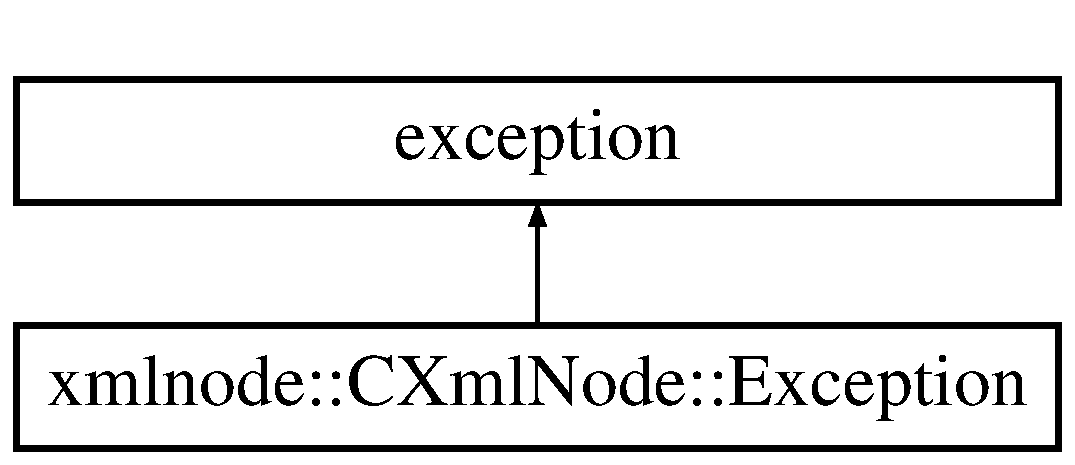
\includegraphics[height=2.000000cm]{classxmlnode_1_1_c_xml_node_1_1_exception}
\end{center}
\end{figure}
\subsection*{Public Types}
\begin{DoxyCompactItemize}
\item 
enum \mbox{\hyperlink{classxmlnode_1_1_c_xml_node_1_1_exception_abdbe07531ef4b19192f1fa2f819ed75f}{Types}} \{ \newline
\mbox{\hyperlink{classxmlnode_1_1_c_xml_node_1_1_exception_abdbe07531ef4b19192f1fa2f819ed75fa22036006e7862ed7f6fc42091f6a3bc8}{None}}, 
\mbox{\hyperlink{classxmlnode_1_1_c_xml_node_1_1_exception_abdbe07531ef4b19192f1fa2f819ed75fa725fdfe67e4fbd5539133a341a5e0a6e}{Unable\+To\+Open}}, 
\mbox{\hyperlink{classxmlnode_1_1_c_xml_node_1_1_exception_abdbe07531ef4b19192f1fa2f819ed75fab4da3fb6cf56910a8302ddb34b697295}{Unable\+To\+Write}}, 
\mbox{\hyperlink{classxmlnode_1_1_c_xml_node_1_1_exception_abdbe07531ef4b19192f1fa2f819ed75fa34828bed7772bc0588f97192c03ea4ad}{Unable\+To\+Create}}, 
\newline
\mbox{\hyperlink{classxmlnode_1_1_c_xml_node_1_1_exception_abdbe07531ef4b19192f1fa2f819ed75fa5e03a8ddc6c8873e07c6a34dc1d7a0e0}{No\+Root}}
 \}
\begin{DoxyCompactList}\small\item\em \mbox{\hyperlink{classxmlnode_1_1_c_xml_node_1_1_exception}{Exception}} types. \end{DoxyCompactList}\end{DoxyCompactItemize}
\subsection*{Public Member Functions}
\begin{DoxyCompactItemize}
\item 
\mbox{\Hypertarget{classxmlnode_1_1_c_xml_node_1_1_exception_ad3078912e0a640db79884170176cb0a8}\label{classxmlnode_1_1_c_xml_node_1_1_exception_ad3078912e0a640db79884170176cb0a8}} 
\mbox{\hyperlink{classxmlnode_1_1_c_xml_node_1_1_exception_ad3078912e0a640db79884170176cb0a8}{Exception}} ()
\begin{DoxyCompactList}\small\item\em Default Constructor. \end{DoxyCompactList}\item 
\mbox{\hyperlink{classxmlnode_1_1_c_xml_node_1_1_exception_aaefc2a485cf66513101ac27c2389c819}{Exception}} (const \mbox{\hyperlink{classxmlnode_1_1_c_xml_node_1_1_exception}{Exception}} \&other)
\begin{DoxyCompactList}\small\item\em Copy Constructor. \end{DoxyCompactList}\item 
\mbox{\hyperlink{classxmlnode_1_1_c_xml_node_1_1_exception}{Exception}} \& \mbox{\hyperlink{classxmlnode_1_1_c_xml_node_1_1_exception_a40c0f5e49e54cd97c4643c71fbc34014}{operator=}} (const \mbox{\hyperlink{classxmlnode_1_1_c_xml_node_1_1_exception}{Exception}} \&other)
\begin{DoxyCompactList}\small\item\em Assignment operator. \end{DoxyCompactList}\item 
\mbox{\hyperlink{classxmlnode_1_1_c_xml_node_1_1_exception_ad660bb87054a9483c0933efbaddfaa55}{Exception}} (\mbox{\hyperlink{classxmlnode_1_1_c_xml_node_1_1_exception_abdbe07531ef4b19192f1fa2f819ed75f}{Types}} type, const std\+::wstring \&msg)
\begin{DoxyCompactList}\small\item\em Constructor. \end{DoxyCompactList}\item 
\mbox{\Hypertarget{classxmlnode_1_1_c_xml_node_1_1_exception_ae22ca483e7821c057dec85f06a5e4d32}\label{classxmlnode_1_1_c_xml_node_1_1_exception_ae22ca483e7821c057dec85f06a5e4d32}} 
virtual \mbox{\hyperlink{classxmlnode_1_1_c_xml_node_1_1_exception_ae22ca483e7821c057dec85f06a5e4d32}{$\sim$\+Exception}} ()
\begin{DoxyCompactList}\small\item\em Destructor. \end{DoxyCompactList}\item 
virtual const char $\ast$ \mbox{\hyperlink{classxmlnode_1_1_c_xml_node_1_1_exception_a55ec16b50448dfa3be05f50051e5ea85}{what}} () const  throw ()
\begin{DoxyCompactList}\small\item\em \mbox{\hyperlink{classxmlnode_1_1_c_xml_node_1_1_exception}{Exception}} message. \end{DoxyCompactList}\item 
std\+::wstring \mbox{\hyperlink{classxmlnode_1_1_c_xml_node_1_1_exception_a29271ad0ec50958663200f60aaae97b2}{Message}} ()
\begin{DoxyCompactList}\small\item\em \mbox{\hyperlink{classxmlnode_1_1_c_xml_node_1_1_exception}{Exception}} message. \end{DoxyCompactList}\item 
\mbox{\hyperlink{classxmlnode_1_1_c_xml_node_1_1_exception_abdbe07531ef4b19192f1fa2f819ed75f}{Types}} \mbox{\hyperlink{classxmlnode_1_1_c_xml_node_1_1_exception_a872eb6da8739faf5424baf6515b43793}{Type}} ()
\begin{DoxyCompactList}\small\item\em \mbox{\hyperlink{classxmlnode_1_1_c_xml_node_1_1_exception}{Exception}} type. \end{DoxyCompactList}\end{DoxyCompactItemize}


\subsection{Detailed Description}
Exceptions for \mbox{\hyperlink{classxmlnode_1_1_c_xml_node}{C\+Xml\+Node}}. 

\subsection{Member Enumeration Documentation}
\mbox{\Hypertarget{classxmlnode_1_1_c_xml_node_1_1_exception_abdbe07531ef4b19192f1fa2f819ed75f}\label{classxmlnode_1_1_c_xml_node_1_1_exception_abdbe07531ef4b19192f1fa2f819ed75f}} 
\index{xmlnode\+::\+C\+Xml\+Node\+::\+Exception@{xmlnode\+::\+C\+Xml\+Node\+::\+Exception}!Types@{Types}}
\index{Types@{Types}!xmlnode\+::\+C\+Xml\+Node\+::\+Exception@{xmlnode\+::\+C\+Xml\+Node\+::\+Exception}}
\subsubsection{\texorpdfstring{Types}{Types}}
{\footnotesize\ttfamily enum \mbox{\hyperlink{classxmlnode_1_1_c_xml_node_1_1_exception_abdbe07531ef4b19192f1fa2f819ed75f}{xmlnode\+::\+C\+Xml\+Node\+::\+Exception\+::\+Types}}}



\mbox{\hyperlink{classxmlnode_1_1_c_xml_node_1_1_exception}{Exception}} types. 

\begin{DoxyEnumFields}{Enumerator}
\raisebox{\heightof{T}}[0pt][0pt]{\index{None@{None}!xmlnode\+::\+C\+Xml\+Node\+::\+Exception@{xmlnode\+::\+C\+Xml\+Node\+::\+Exception}}\index{xmlnode\+::\+C\+Xml\+Node\+::\+Exception@{xmlnode\+::\+C\+Xml\+Node\+::\+Exception}!None@{None}}}\mbox{\Hypertarget{classxmlnode_1_1_c_xml_node_1_1_exception_abdbe07531ef4b19192f1fa2f819ed75fa22036006e7862ed7f6fc42091f6a3bc8}\label{classxmlnode_1_1_c_xml_node_1_1_exception_abdbe07531ef4b19192f1fa2f819ed75fa22036006e7862ed7f6fc42091f6a3bc8}} 
None&No exception type indicated. \\
\hline

\raisebox{\heightof{T}}[0pt][0pt]{\index{Unable\+To\+Open@{Unable\+To\+Open}!xmlnode\+::\+C\+Xml\+Node\+::\+Exception@{xmlnode\+::\+C\+Xml\+Node\+::\+Exception}}\index{xmlnode\+::\+C\+Xml\+Node\+::\+Exception@{xmlnode\+::\+C\+Xml\+Node\+::\+Exception}!Unable\+To\+Open@{Unable\+To\+Open}}}\mbox{\Hypertarget{classxmlnode_1_1_c_xml_node_1_1_exception_abdbe07531ef4b19192f1fa2f819ed75fa725fdfe67e4fbd5539133a341a5e0a6e}\label{classxmlnode_1_1_c_xml_node_1_1_exception_abdbe07531ef4b19192f1fa2f819ed75fa725fdfe67e4fbd5539133a341a5e0a6e}} 
Unable\+To\+Open&Unable to open file to read. \\
\hline

\raisebox{\heightof{T}}[0pt][0pt]{\index{Unable\+To\+Write@{Unable\+To\+Write}!xmlnode\+::\+C\+Xml\+Node\+::\+Exception@{xmlnode\+::\+C\+Xml\+Node\+::\+Exception}}\index{xmlnode\+::\+C\+Xml\+Node\+::\+Exception@{xmlnode\+::\+C\+Xml\+Node\+::\+Exception}!Unable\+To\+Write@{Unable\+To\+Write}}}\mbox{\Hypertarget{classxmlnode_1_1_c_xml_node_1_1_exception_abdbe07531ef4b19192f1fa2f819ed75fab4da3fb6cf56910a8302ddb34b697295}\label{classxmlnode_1_1_c_xml_node_1_1_exception_abdbe07531ef4b19192f1fa2f819ed75fab4da3fb6cf56910a8302ddb34b697295}} 
Unable\+To\+Write&Unable to open file to write. \\
\hline

\raisebox{\heightof{T}}[0pt][0pt]{\index{Unable\+To\+Create@{Unable\+To\+Create}!xmlnode\+::\+C\+Xml\+Node\+::\+Exception@{xmlnode\+::\+C\+Xml\+Node\+::\+Exception}}\index{xmlnode\+::\+C\+Xml\+Node\+::\+Exception@{xmlnode\+::\+C\+Xml\+Node\+::\+Exception}!Unable\+To\+Create@{Unable\+To\+Create}}}\mbox{\Hypertarget{classxmlnode_1_1_c_xml_node_1_1_exception_abdbe07531ef4b19192f1fa2f819ed75fa34828bed7772bc0588f97192c03ea4ad}\label{classxmlnode_1_1_c_xml_node_1_1_exception_abdbe07531ef4b19192f1fa2f819ed75fa34828bed7772bc0588f97192c03ea4ad}} 
Unable\+To\+Create&Unable to create X\+ML document. \\
\hline

\raisebox{\heightof{T}}[0pt][0pt]{\index{No\+Root@{No\+Root}!xmlnode\+::\+C\+Xml\+Node\+::\+Exception@{xmlnode\+::\+C\+Xml\+Node\+::\+Exception}}\index{xmlnode\+::\+C\+Xml\+Node\+::\+Exception@{xmlnode\+::\+C\+Xml\+Node\+::\+Exception}!No\+Root@{No\+Root}}}\mbox{\Hypertarget{classxmlnode_1_1_c_xml_node_1_1_exception_abdbe07531ef4b19192f1fa2f819ed75fa5e03a8ddc6c8873e07c6a34dc1d7a0e0}\label{classxmlnode_1_1_c_xml_node_1_1_exception_abdbe07531ef4b19192f1fa2f819ed75fa5e03a8ddc6c8873e07c6a34dc1d7a0e0}} 
No\+Root&Not X\+ML document root node. \\
\hline

\end{DoxyEnumFields}


\subsection{Constructor \& Destructor Documentation}
\mbox{\Hypertarget{classxmlnode_1_1_c_xml_node_1_1_exception_aaefc2a485cf66513101ac27c2389c819}\label{classxmlnode_1_1_c_xml_node_1_1_exception_aaefc2a485cf66513101ac27c2389c819}} 
\index{xmlnode\+::\+C\+Xml\+Node\+::\+Exception@{xmlnode\+::\+C\+Xml\+Node\+::\+Exception}!Exception@{Exception}}
\index{Exception@{Exception}!xmlnode\+::\+C\+Xml\+Node\+::\+Exception@{xmlnode\+::\+C\+Xml\+Node\+::\+Exception}}
\subsubsection{\texorpdfstring{Exception()}{Exception()}\hspace{0.1cm}{\footnotesize\ttfamily [1/2]}}
{\footnotesize\ttfamily xmlnode\+::\+C\+Xml\+Node\+::\+Exception\+::\+Exception (\begin{DoxyParamCaption}\item[{const \mbox{\hyperlink{classxmlnode_1_1_c_xml_node_1_1_exception}{Exception}} \&}]{other }\end{DoxyParamCaption})\hspace{0.3cm}{\ttfamily [inline]}}



Copy Constructor. 


\begin{DoxyParams}{Parameters}
{\em other} & Object to copy \\
\hline
\end{DoxyParams}
\mbox{\Hypertarget{classxmlnode_1_1_c_xml_node_1_1_exception_ad660bb87054a9483c0933efbaddfaa55}\label{classxmlnode_1_1_c_xml_node_1_1_exception_ad660bb87054a9483c0933efbaddfaa55}} 
\index{xmlnode\+::\+C\+Xml\+Node\+::\+Exception@{xmlnode\+::\+C\+Xml\+Node\+::\+Exception}!Exception@{Exception}}
\index{Exception@{Exception}!xmlnode\+::\+C\+Xml\+Node\+::\+Exception@{xmlnode\+::\+C\+Xml\+Node\+::\+Exception}}
\subsubsection{\texorpdfstring{Exception()}{Exception()}\hspace{0.1cm}{\footnotesize\ttfamily [2/2]}}
{\footnotesize\ttfamily xmlnode\+::\+C\+Xml\+Node\+::\+Exception\+::\+Exception (\begin{DoxyParamCaption}\item[{\mbox{\hyperlink{classxmlnode_1_1_c_xml_node_1_1_exception_abdbe07531ef4b19192f1fa2f819ed75f}{Types}}}]{type,  }\item[{const std\+::wstring \&}]{msg }\end{DoxyParamCaption})\hspace{0.3cm}{\ttfamily [inline]}}



Constructor. 


\begin{DoxyParams}{Parameters}
{\em type} & \mbox{\hyperlink{classxmlnode_1_1_c_xml_node_1_1_exception}{Exception}} type \\
\hline
{\em msg} & Message associated with exception \\
\hline
\end{DoxyParams}


\subsection{Member Function Documentation}
\mbox{\Hypertarget{classxmlnode_1_1_c_xml_node_1_1_exception_a29271ad0ec50958663200f60aaae97b2}\label{classxmlnode_1_1_c_xml_node_1_1_exception_a29271ad0ec50958663200f60aaae97b2}} 
\index{xmlnode\+::\+C\+Xml\+Node\+::\+Exception@{xmlnode\+::\+C\+Xml\+Node\+::\+Exception}!Message@{Message}}
\index{Message@{Message}!xmlnode\+::\+C\+Xml\+Node\+::\+Exception@{xmlnode\+::\+C\+Xml\+Node\+::\+Exception}}
\subsubsection{\texorpdfstring{Message()}{Message()}}
{\footnotesize\ttfamily std\+::wstring xmlnode\+::\+C\+Xml\+Node\+::\+Exception\+::\+Message (\begin{DoxyParamCaption}{ }\end{DoxyParamCaption})\hspace{0.3cm}{\ttfamily [inline]}}



\mbox{\hyperlink{classxmlnode_1_1_c_xml_node_1_1_exception}{Exception}} message. 

\begin{DoxyReturn}{Returns}
\mbox{\hyperlink{classxmlnode_1_1_c_xml_node_1_1_exception}{Exception}} message 
\end{DoxyReturn}
\mbox{\Hypertarget{classxmlnode_1_1_c_xml_node_1_1_exception_a40c0f5e49e54cd97c4643c71fbc34014}\label{classxmlnode_1_1_c_xml_node_1_1_exception_a40c0f5e49e54cd97c4643c71fbc34014}} 
\index{xmlnode\+::\+C\+Xml\+Node\+::\+Exception@{xmlnode\+::\+C\+Xml\+Node\+::\+Exception}!operator=@{operator=}}
\index{operator=@{operator=}!xmlnode\+::\+C\+Xml\+Node\+::\+Exception@{xmlnode\+::\+C\+Xml\+Node\+::\+Exception}}
\subsubsection{\texorpdfstring{operator=()}{operator=()}}
{\footnotesize\ttfamily \mbox{\hyperlink{classxmlnode_1_1_c_xml_node_1_1_exception}{Exception}}\& xmlnode\+::\+C\+Xml\+Node\+::\+Exception\+::operator= (\begin{DoxyParamCaption}\item[{const \mbox{\hyperlink{classxmlnode_1_1_c_xml_node_1_1_exception}{Exception}} \&}]{other }\end{DoxyParamCaption})\hspace{0.3cm}{\ttfamily [inline]}}



Assignment operator. 


\begin{DoxyParams}{Parameters}
{\em other} & Object to copy \\
\hline
\end{DoxyParams}
\begin{DoxyReturn}{Returns}
Reference to this object 
\end{DoxyReturn}
\mbox{\Hypertarget{classxmlnode_1_1_c_xml_node_1_1_exception_a872eb6da8739faf5424baf6515b43793}\label{classxmlnode_1_1_c_xml_node_1_1_exception_a872eb6da8739faf5424baf6515b43793}} 
\index{xmlnode\+::\+C\+Xml\+Node\+::\+Exception@{xmlnode\+::\+C\+Xml\+Node\+::\+Exception}!Type@{Type}}
\index{Type@{Type}!xmlnode\+::\+C\+Xml\+Node\+::\+Exception@{xmlnode\+::\+C\+Xml\+Node\+::\+Exception}}
\subsubsection{\texorpdfstring{Type()}{Type()}}
{\footnotesize\ttfamily \mbox{\hyperlink{classxmlnode_1_1_c_xml_node_1_1_exception_abdbe07531ef4b19192f1fa2f819ed75f}{Types}} xmlnode\+::\+C\+Xml\+Node\+::\+Exception\+::\+Type (\begin{DoxyParamCaption}{ }\end{DoxyParamCaption})\hspace{0.3cm}{\ttfamily [inline]}}



\mbox{\hyperlink{classxmlnode_1_1_c_xml_node_1_1_exception}{Exception}} type. 

\begin{DoxyReturn}{Returns}
\mbox{\hyperlink{classxmlnode_1_1_c_xml_node_1_1_exception}{Exception}} type of type \mbox{\hyperlink{classxmlnode_1_1_c_xml_node_1_1_exception_abdbe07531ef4b19192f1fa2f819ed75f}{C\+Xml\+Node\+::\+Exception\+::\+Types}} 
\end{DoxyReturn}
\mbox{\Hypertarget{classxmlnode_1_1_c_xml_node_1_1_exception_a55ec16b50448dfa3be05f50051e5ea85}\label{classxmlnode_1_1_c_xml_node_1_1_exception_a55ec16b50448dfa3be05f50051e5ea85}} 
\index{xmlnode\+::\+C\+Xml\+Node\+::\+Exception@{xmlnode\+::\+C\+Xml\+Node\+::\+Exception}!what@{what}}
\index{what@{what}!xmlnode\+::\+C\+Xml\+Node\+::\+Exception@{xmlnode\+::\+C\+Xml\+Node\+::\+Exception}}
\subsubsection{\texorpdfstring{what()}{what()}}
{\footnotesize\ttfamily virtual const char$\ast$ xmlnode\+::\+C\+Xml\+Node\+::\+Exception\+::what (\begin{DoxyParamCaption}{ }\end{DoxyParamCaption}) const throw  ) \hspace{0.3cm}{\ttfamily [inline]}, {\ttfamily [virtual]}}



\mbox{\hyperlink{classxmlnode_1_1_c_xml_node_1_1_exception}{Exception}} message. 

More verbose exception messages are provided in Unicode as they should be by the \mbox{\hyperlink{classxmlnode_1_1_c_xml_node_1_1_exception_a29271ad0ec50958663200f60aaae97b2}{Message()}} function. \begin{DoxyReturn}{Returns}
\char`\"{}\+C\+Xml\+Node exception\char`\"{} 
\end{DoxyReturn}


The documentation for this class was generated from the following file\+:\begin{DoxyCompactItemize}
\item 
\mbox{\hyperlink{_xml_node_8h}{Xml\+Node.\+h}}\end{DoxyCompactItemize}

\hypertarget{classxmlnode_1_1_c_xml_node_1_1_iterator}{}\section{xmlnode\+:\+:C\+Xml\+Node\+:\+:Iterator Class Reference}
\label{classxmlnode_1_1_c_xml_node_1_1_iterator}\index{xmlnode\+::\+C\+Xml\+Node\+::\+Iterator@{xmlnode\+::\+C\+Xml\+Node\+::\+Iterator}}


Support for iterating over the children of a node.  




{\ttfamily \#include $<$Xml\+Node.\+h$>$}

\subsection*{Public Member Functions}
\begin{DoxyCompactItemize}
\item 
bool \mbox{\hyperlink{classxmlnode_1_1_c_xml_node_1_1_iterator_a55c86e64262a6ef16e253f2aef70578c}{operator!=}} (const \mbox{\hyperlink{classxmlnode_1_1_c_xml_node_1_1_iterator}{Iterator}} \&other) const
\begin{DoxyCompactList}\small\item\em Test to see if two iterator are at the same location. \end{DoxyCompactList}\item 
std\+::shared\+\_\+ptr$<$ \mbox{\hyperlink{classxmlnode_1_1_c_xml_node}{C\+Xml\+Node}} $>$ \mbox{\hyperlink{classxmlnode_1_1_c_xml_node_1_1_iterator_a6d255a513c60c7de55a01c5eb626bf6d}{operator$\ast$}} ()
\begin{DoxyCompactList}\small\item\em Operation $\ast$ for the iterator. \end{DoxyCompactList}\item 
const \mbox{\hyperlink{classxmlnode_1_1_c_xml_node_1_1_iterator}{Iterator}} \& \mbox{\hyperlink{classxmlnode_1_1_c_xml_node_1_1_iterator_aefa7392f7c198dcf907d8458fbf0db1a}{operator++}} ()
\begin{DoxyCompactList}\small\item\em Advance to the next item in the collection. \end{DoxyCompactList}\end{DoxyCompactItemize}
\subsection*{Friends}
\begin{DoxyCompactItemize}
\item 
\mbox{\Hypertarget{classxmlnode_1_1_c_xml_node_1_1_iterator_a770307dc9d4e2e7005bcf200bae3066a}\label{classxmlnode_1_1_c_xml_node_1_1_iterator_a770307dc9d4e2e7005bcf200bae3066a}} 
class \mbox{\hyperlink{classxmlnode_1_1_c_xml_node_1_1_iterator_a770307dc9d4e2e7005bcf200bae3066a}{C\+Xml\+Node}}
\begin{DoxyCompactList}\small\item\em Friend class. \end{DoxyCompactList}\end{DoxyCompactItemize}


\subsection{Detailed Description}
Support for iterating over the children of a node. 

\subsection{Member Function Documentation}
\mbox{\Hypertarget{classxmlnode_1_1_c_xml_node_1_1_iterator_a55c86e64262a6ef16e253f2aef70578c}\label{classxmlnode_1_1_c_xml_node_1_1_iterator_a55c86e64262a6ef16e253f2aef70578c}} 
\index{xmlnode\+::\+C\+Xml\+Node\+::\+Iterator@{xmlnode\+::\+C\+Xml\+Node\+::\+Iterator}!operator"!=@{operator"!=}}
\index{operator"!=@{operator"!=}!xmlnode\+::\+C\+Xml\+Node\+::\+Iterator@{xmlnode\+::\+C\+Xml\+Node\+::\+Iterator}}
\subsubsection{\texorpdfstring{operator"!=()}{operator!=()}}
{\footnotesize\ttfamily bool xmlnode\+::\+C\+Xml\+Node\+::\+Iterator\+::operator!= (\begin{DoxyParamCaption}\item[{const \mbox{\hyperlink{classxmlnode_1_1_c_xml_node_1_1_iterator}{Iterator}} \&}]{other }\end{DoxyParamCaption}) const\hspace{0.3cm}{\ttfamily [inline]}}



Test to see if two iterator are at the same location. 


\begin{DoxyParams}{Parameters}
{\em other} & The other object we are testing against \\
\hline
\end{DoxyParams}
\begin{DoxyReturn}{Returns}
true if they are equal. 
\end{DoxyReturn}
\mbox{\Hypertarget{classxmlnode_1_1_c_xml_node_1_1_iterator_a6d255a513c60c7de55a01c5eb626bf6d}\label{classxmlnode_1_1_c_xml_node_1_1_iterator_a6d255a513c60c7de55a01c5eb626bf6d}} 
\index{xmlnode\+::\+C\+Xml\+Node\+::\+Iterator@{xmlnode\+::\+C\+Xml\+Node\+::\+Iterator}!operator$\ast$@{operator$\ast$}}
\index{operator$\ast$@{operator$\ast$}!xmlnode\+::\+C\+Xml\+Node\+::\+Iterator@{xmlnode\+::\+C\+Xml\+Node\+::\+Iterator}}
\subsubsection{\texorpdfstring{operator$\ast$()}{operator*()}}
{\footnotesize\ttfamily std\+::shared\+\_\+ptr$<$ \mbox{\hyperlink{classxmlnode_1_1_c_xml_node}{C\+Xml\+Node}} $>$ C\+Xml\+Node\+::\+Iterator\+::operator$\ast$ (\begin{DoxyParamCaption}{ }\end{DoxyParamCaption})}



Operation $\ast$ for the iterator. 

Indiates the child that is the current iterator reference.

\begin{DoxyReturn}{Returns}
Pointer to child node. 
\end{DoxyReturn}
\mbox{\Hypertarget{classxmlnode_1_1_c_xml_node_1_1_iterator_aefa7392f7c198dcf907d8458fbf0db1a}\label{classxmlnode_1_1_c_xml_node_1_1_iterator_aefa7392f7c198dcf907d8458fbf0db1a}} 
\index{xmlnode\+::\+C\+Xml\+Node\+::\+Iterator@{xmlnode\+::\+C\+Xml\+Node\+::\+Iterator}!operator++@{operator++}}
\index{operator++@{operator++}!xmlnode\+::\+C\+Xml\+Node\+::\+Iterator@{xmlnode\+::\+C\+Xml\+Node\+::\+Iterator}}
\subsubsection{\texorpdfstring{operator++()}{operator++()}}
{\footnotesize\ttfamily const \mbox{\hyperlink{classxmlnode_1_1_c_xml_node_1_1_iterator}{Iterator}}\& xmlnode\+::\+C\+Xml\+Node\+::\+Iterator\+::operator++ (\begin{DoxyParamCaption}{ }\end{DoxyParamCaption})\hspace{0.3cm}{\ttfamily [inline]}}



Advance to the next item in the collection. 

\begin{DoxyReturn}{Returns}
Reference to this iterator. 
\end{DoxyReturn}


The documentation for this class was generated from the following files\+:\begin{DoxyCompactItemize}
\item 
\mbox{\hyperlink{_xml_node_8h}{Xml\+Node.\+h}}\item 
\mbox{\hyperlink{_xml_node_8cpp}{Xml\+Node.\+cpp}}\end{DoxyCompactItemize}

\chapter{File Documentation}
\hypertarget{_aquarium_8cpp}{}\section{Aquarium.\+cpp File Reference}
\label{_aquarium_8cpp}\index{Aquarium.\+cpp@{Aquarium.\+cpp}}
{\ttfamily \#include \char`\"{}stdafx.\+h\char`\"{}}\newline
{\ttfamily \#include \char`\"{}Aquarium.\+h\char`\"{}}\newline
{\ttfamily \#include $<$memory$>$}\newline


\subsection{Detailed Description}
\begin{DoxyAuthor}{Author}
Mark Maroki 
\end{DoxyAuthor}

\hypertarget{_aquarium_8h}{}\section{Aquarium.\+h File Reference}
\label{_aquarium_8h}\index{Aquarium.\+h@{Aquarium.\+h}}
{\ttfamily \#include $<$memory$>$}\newline
\subsection*{Classes}
\begin{DoxyCompactItemize}
\item 
class \mbox{\hyperlink{class_c_aquarium}{C\+Aquarium}}
\end{DoxyCompactItemize}


\subsection{Detailed Description}
\begin{DoxyAuthor}{Author}
Mark Maroki Class that implements the Aquarium window. 
\end{DoxyAuthor}

\hypertarget{_child_view_8cpp}{}\section{Child\+View.\+cpp File Reference}
\label{_child_view_8cpp}\index{Child\+View.\+cpp@{Child\+View.\+cpp}}
{\ttfamily \#include \char`\"{}stdafx.\+h\char`\"{}}\newline
{\ttfamily \#include \char`\"{}Step2.\+h\char`\"{}}\newline
{\ttfamily \#include \char`\"{}Child\+View.\+h\char`\"{}}\newline


\subsection{Detailed Description}
\begin{DoxyAuthor}{Author}
Mark Maroki 
\end{DoxyAuthor}

\hypertarget{_child_view_8h}{}\section{Child\+View.\+h File Reference}
\label{_child_view_8h}\index{Child\+View.\+h@{Child\+View.\+h}}
{\ttfamily \#include \char`\"{}Aquarium.\+h\char`\"{}}\newline
\subsection*{Classes}
\begin{DoxyCompactItemize}
\item 
class \mbox{\hyperlink{class_c_child_view}{C\+Child\+View}}
\end{DoxyCompactItemize}


\subsection{Detailed Description}
\begin{DoxyAuthor}{Author}
Mark Maroki
\end{DoxyAuthor}
Class that implements child window the program draws in.

The window is a child of the main frame, which holds the window, the menu bar, and the status bar. 
\hypertarget{_decor_castle_8h}{}\section{Decor\+Castle.\+h File Reference}
\label{_decor_castle_8h}\index{Decor\+Castle.\+h@{Decor\+Castle.\+h}}
{\ttfamily \#include $<$memory$>$}\newline
{\ttfamily \#include \char`\"{}Item.\+h\char`\"{}}\newline
\subsection*{Classes}
\begin{DoxyCompactItemize}
\item 
class \mbox{\hyperlink{class_c_decor_castle}{C\+Decor\+Castle}}
\end{DoxyCompactItemize}


\subsection{Detailed Description}
\begin{DoxyAuthor}{Author}
Mark Maroki
\end{DoxyAuthor}
Class that implements a Decor Castle. 
\hypertarget{_double_buffer_d_c_8h}{}\section{Double\+Buffer\+D\+C.\+h File Reference}
\label{_double_buffer_d_c_8h}\index{Double\+Buffer\+D\+C.\+h@{Double\+Buffer\+D\+C.\+h}}


Custom device context that supports double buffering.  




\subsection{Detailed Description}
Custom device context that supports double buffering. 


\hypertarget{_fish_8cpp}{}\section{Fish.\+cpp File Reference}
\label{_fish_8cpp}\index{Fish.\+cpp@{Fish.\+cpp}}
{\ttfamily \#include \char`\"{}stdafx.\+h\char`\"{}}\newline
{\ttfamily \#include \char`\"{}Fish.\+h\char`\"{}}\newline
{\ttfamily \#include \char`\"{}Xml\+Node.\+h\char`\"{}}\newline
\subsection*{Variables}
\begin{DoxyCompactItemize}
\item 
const double \mbox{\hyperlink{_fish_8cpp_a84803bf135ee6b4290f36716edeea269}{Max\+SpeedX}} = 50
\item 
const double \mbox{\hyperlink{_fish_8cpp_a0000b7225e39d6d459ab7e7ae20c49e1}{Max\+SpeedY}} = 50
\item 
const double \mbox{\hyperlink{_fish_8cpp_af1c1a50745fc8f450af923903963cb6e}{Min\+SpeedX}} = 1
\item 
const double \mbox{\hyperlink{_fish_8cpp_a2b4f51aa4f192839d41e84ce33e455b1}{Min\+SpeedY}} = 1
\item 
\mbox{\Hypertarget{_fish_8cpp_aef33146937ae35308e4b8526fb0b2579}\label{_fish_8cpp_aef33146937ae35308e4b8526fb0b2579}} 
const int \mbox{\hyperlink{_fish_8cpp_aef33146937ae35308e4b8526fb0b2579}{Background\+Distance}} = 10
\begin{DoxyCompactList}\small\item\em Distance of 25 pixels from end of background. \end{DoxyCompactList}\item 
\mbox{\Hypertarget{_fish_8cpp_a04df4f617e974c20844df36752d3d50c}\label{_fish_8cpp_a04df4f617e974c20844df36752d3d50c}} 
const double \mbox{\hyperlink{_fish_8cpp_a04df4f617e974c20844df36752d3d50c}{Aquarium\+Origin}} = 0
\begin{DoxyCompactList}\small\item\em Beginning of the aquarium for the x coordinate. \end{DoxyCompactList}\end{DoxyCompactItemize}


\subsection{Detailed Description}
Attributes and functionality for fish \begin{DoxyAuthor}{Author}
Mark Maroki 
\end{DoxyAuthor}


\subsection{Variable Documentation}
\mbox{\Hypertarget{_fish_8cpp_a84803bf135ee6b4290f36716edeea269}\label{_fish_8cpp_a84803bf135ee6b4290f36716edeea269}} 
\index{Fish.\+cpp@{Fish.\+cpp}!Max\+SpeedX@{Max\+SpeedX}}
\index{Max\+SpeedX@{Max\+SpeedX}!Fish.\+cpp@{Fish.\+cpp}}
\subsubsection{\texorpdfstring{Max\+SpeedX}{MaxSpeedX}}
{\footnotesize\ttfamily const double Max\+SpeedX = 50}

Maximum speed in the X direction in in pixels per second \mbox{\Hypertarget{_fish_8cpp_a0000b7225e39d6d459ab7e7ae20c49e1}\label{_fish_8cpp_a0000b7225e39d6d459ab7e7ae20c49e1}} 
\index{Fish.\+cpp@{Fish.\+cpp}!Max\+SpeedY@{Max\+SpeedY}}
\index{Max\+SpeedY@{Max\+SpeedY}!Fish.\+cpp@{Fish.\+cpp}}
\subsubsection{\texorpdfstring{Max\+SpeedY}{MaxSpeedY}}
{\footnotesize\ttfamily const double Max\+SpeedY = 50}

Maximum speed in the Y direction in in pixels per second \mbox{\Hypertarget{_fish_8cpp_af1c1a50745fc8f450af923903963cb6e}\label{_fish_8cpp_af1c1a50745fc8f450af923903963cb6e}} 
\index{Fish.\+cpp@{Fish.\+cpp}!Min\+SpeedX@{Min\+SpeedX}}
\index{Min\+SpeedX@{Min\+SpeedX}!Fish.\+cpp@{Fish.\+cpp}}
\subsubsection{\texorpdfstring{Min\+SpeedX}{MinSpeedX}}
{\footnotesize\ttfamily const double Min\+SpeedX = 1}

Minimum speed in the X direction in pixels per second \mbox{\Hypertarget{_fish_8cpp_a2b4f51aa4f192839d41e84ce33e455b1}\label{_fish_8cpp_a2b4f51aa4f192839d41e84ce33e455b1}} 
\index{Fish.\+cpp@{Fish.\+cpp}!Min\+SpeedY@{Min\+SpeedY}}
\index{Min\+SpeedY@{Min\+SpeedY}!Fish.\+cpp@{Fish.\+cpp}}
\subsubsection{\texorpdfstring{Min\+SpeedY}{MinSpeedY}}
{\footnotesize\ttfamily const double Min\+SpeedY = 1}

Minimum speed in the Y direction in pixels per second 
\hypertarget{_fish_beta_8cpp}{}\section{Fish\+Beta.\+cpp File Reference}
\label{_fish_beta_8cpp}\index{Fish\+Beta.\+cpp@{Fish\+Beta.\+cpp}}
{\ttfamily \#include \char`\"{}stdafx.\+h\char`\"{}}\newline
{\ttfamily \#include \char`\"{}Fish\+Beta.\+h\char`\"{}}\newline


\subsection{Detailed Description}
\begin{DoxyAuthor}{Author}
Mark Maroki 
\end{DoxyAuthor}

\hypertarget{_fish_beta_8h}{}\section{Fish\+Beta.\+h File Reference}
\label{_fish_beta_8h}\index{Fish\+Beta.\+h@{Fish\+Beta.\+h}}
{\ttfamily \#include \char`\"{}Item.\+h\char`\"{}}\newline
\subsection*{Classes}
\begin{DoxyCompactItemize}
\item 
class \mbox{\hyperlink{class_c_fish_beta}{C\+Fish\+Beta}}
\end{DoxyCompactItemize}


\subsection{Detailed Description}
\begin{DoxyAuthor}{Author}
Mark Maroki Beta Fish class derived from Items class. 
\end{DoxyAuthor}

\hypertarget{_fish_dory_8cpp}{}\section{Fish\+Dory.\+cpp File Reference}
\label{_fish_dory_8cpp}\index{Fish\+Dory.\+cpp@{Fish\+Dory.\+cpp}}
{\ttfamily \#include \char`\"{}stdafx.\+h\char`\"{}}\newline
{\ttfamily \#include \char`\"{}Fish\+Dory.\+h\char`\"{}}\newline
{\ttfamily \#include \char`\"{}Xml\+Node.\+h\char`\"{}}\newline
\subsection*{Variables}
\begin{DoxyCompactItemize}
\item 
\mbox{\Hypertarget{_fish_dory_8cpp_a81330bfdb7ff6eb8410e8a91bd99032c}\label{_fish_dory_8cpp_a81330bfdb7ff6eb8410e8a91bd99032c}} 
const wstring \mbox{\hyperlink{_fish_dory_8cpp_a81330bfdb7ff6eb8410e8a91bd99032c}{Fish\+Dory\+Image\+Name}} = L\char`\"{}images/dory.\+png\char`\"{}
\begin{DoxyCompactList}\small\item\em Fish filename. \end{DoxyCompactList}\end{DoxyCompactItemize}


\subsection{Detailed Description}
\begin{DoxyAuthor}{Author}
Mark Maroki 
\end{DoxyAuthor}

\hypertarget{_fish_karp_8cpp}{}\section{Fish\+Karp.\+cpp File Reference}
\label{_fish_karp_8cpp}\index{Fish\+Karp.\+cpp@{Fish\+Karp.\+cpp}}
{\ttfamily \#include \char`\"{}stdafx.\+h\char`\"{}}\newline
{\ttfamily \#include $<$string$>$}\newline
{\ttfamily \#include \char`\"{}Fish\+Karp.\+h\char`\"{}}\newline
{\ttfamily \#include \char`\"{}Aquarium.\+h\char`\"{}}\newline
\subsection*{Variables}
\begin{DoxyCompactItemize}
\item 
\mbox{\Hypertarget{_fish_karp_8cpp_a4ecd408816d32435929afba5e9772ce3}\label{_fish_karp_8cpp_a4ecd408816d32435929afba5e9772ce3}} 
const wstring \mbox{\hyperlink{_fish_karp_8cpp_a4ecd408816d32435929afba5e9772ce3}{Fish\+Karp\+Image\+Name}} = L\char`\"{}images/carp.\+png\char`\"{}
\begin{DoxyCompactList}\small\item\em Fish filename. \end{DoxyCompactList}\end{DoxyCompactItemize}


\subsection{Detailed Description}
\begin{DoxyAuthor}{Author}
Mark Maroki 
\end{DoxyAuthor}

\hypertarget{_fish_karp_8h}{}\section{Fish\+Karp.\+h File Reference}
\label{_fish_karp_8h}\index{Fish\+Karp.\+h@{Fish\+Karp.\+h}}
{\ttfamily \#include $<$memory$>$}\newline
{\ttfamily \#include \char`\"{}Xml\+Node.\+h\char`\"{}}\newline
{\ttfamily \#include \char`\"{}Item.\+h\char`\"{}}\newline
{\ttfamily \#include \char`\"{}Fish.\+h\char`\"{}}\newline
\subsection*{Classes}
\begin{DoxyCompactItemize}
\item 
class \mbox{\hyperlink{class_c_fish_karp}{C\+Fish\+Karp}}
\end{DoxyCompactItemize}


\subsection{Detailed Description}
\begin{DoxyAuthor}{Author}
Mark Maroki
\end{DoxyAuthor}
Class the implements a Karp fish 
\hypertarget{_fish_nemo_8cpp}{}\section{Fish\+Nemo.\+cpp File Reference}
\label{_fish_nemo_8cpp}\index{Fish\+Nemo.\+cpp@{Fish\+Nemo.\+cpp}}
{\ttfamily \#include \char`\"{}stdafx.\+h\char`\"{}}\newline
{\ttfamily \#include $<$string$>$}\newline
{\ttfamily \#include \char`\"{}Fish\+Nemo.\+h\char`\"{}}\newline
\subsection*{Variables}
\begin{DoxyCompactItemize}
\item 
\mbox{\Hypertarget{_fish_nemo_8cpp_a49911ce0d27ea7b0c3f516e747e0e7b3}\label{_fish_nemo_8cpp_a49911ce0d27ea7b0c3f516e747e0e7b3}} 
const wstring \mbox{\hyperlink{_fish_nemo_8cpp_a49911ce0d27ea7b0c3f516e747e0e7b3}{Fish\+Nemo\+Image\+Name}} = L\char`\"{}images/nemo.\+png\char`\"{}
\begin{DoxyCompactList}\small\item\em Fish filename. \end{DoxyCompactList}\end{DoxyCompactItemize}


\subsection{Detailed Description}
\begin{DoxyAuthor}{Author}
Mark Maroki 
\end{DoxyAuthor}

\hypertarget{_fish_nemo_8h}{}\section{Fish\+Nemo.\+h File Reference}
\label{_fish_nemo_8h}\index{Fish\+Nemo.\+h@{Fish\+Nemo.\+h}}
{\ttfamily \#include $<$memory$>$}\newline
{\ttfamily \#include \char`\"{}Xml\+Node.\+h\char`\"{}}\newline
{\ttfamily \#include \char`\"{}Item.\+h\char`\"{}}\newline
{\ttfamily \#include \char`\"{}Fish.\+h\char`\"{}}\newline
\subsection*{Classes}
\begin{DoxyCompactItemize}
\item 
class \mbox{\hyperlink{class_c_fish_nemo}{C\+Fish\+Nemo}}
\end{DoxyCompactItemize}


\subsection{Detailed Description}
\begin{DoxyAuthor}{Author}
Charles B. Owen
\end{DoxyAuthor}
Class the implements a Nemo fish 
\hypertarget{_item_8cpp}{}\section{Item.\+cpp File Reference}
\label{_item_8cpp}\index{Item.\+cpp@{Item.\+cpp}}
{\ttfamily \#include \char`\"{}stdafx.\+h\char`\"{}}\newline
{\ttfamily \#include \char`\"{}Item.\+h\char`\"{}}\newline
{\ttfamily \#include \char`\"{}Aquarium.\+h\char`\"{}}\newline


\subsection{Detailed Description}
\begin{DoxyAuthor}{Author}
Mark Maroki 
\end{DoxyAuthor}

\hypertarget{_item_8h}{}\section{Item.\+h File Reference}
\label{_item_8h}\index{Item.\+h@{Item.\+h}}
\subsection*{Classes}
\begin{DoxyCompactItemize}
\item 
class \mbox{\hyperlink{class_c_item}{C\+Item}}
\end{DoxyCompactItemize}


\subsection{Detailed Description}
Item Class is used to track the Items in the Aquarium. Therefore is a child? \begin{DoxyAuthor}{Author}
Mark Maroki 
\end{DoxyAuthor}

\hypertarget{_xml_node_8cpp}{}\section{Xml\+Node.\+cpp File Reference}
\label{_xml_node_8cpp}\index{Xml\+Node.\+cpp@{Xml\+Node.\+cpp}}


Class that implements a wrapper for msxml nodes.  


{\ttfamily \#include \char`\"{}stdafx.\+h\char`\"{}}\newline
{\ttfamily \#include \char`\"{}Xml\+Node.\+h\char`\"{}}\newline


\subsection{Detailed Description}
Class that implements a wrapper for msxml nodes. 

\begin{DoxyAuthor}{Author}
Charles B. Owen 
\end{DoxyAuthor}
\begin{DoxyVersion}{Version}
1.\+01 07-\/16-\/2014 

1.\+02 07-\/17-\/2014 

1.\+03 07-\/17-\/2014 
\end{DoxyVersion}

\hypertarget{_xml_node_8h}{}\section{Xml\+Node.\+h File Reference}
\label{_xml_node_8h}\index{Xml\+Node.\+h@{Xml\+Node.\+h}}


Class that implements a wrapper for msxml nodes.  


{\ttfamily \#include $<$Ms\+Xml6.\+h$>$}\newline
{\ttfamily \#include $<$memory$>$}\newline
{\ttfamily \#include $<$string$>$}\newline
{\ttfamily \#include $<$exception$>$}\newline
\subsection*{Classes}
\begin{DoxyCompactItemize}
\item 
class \mbox{\hyperlink{classxmlnode_1_1_c_xml_node}{xmlnode\+::\+C\+Xml\+Node}}
\begin{DoxyCompactList}\small\item\em A wrapper for msxml nodes. \end{DoxyCompactList}\item 
class \mbox{\hyperlink{classxmlnode_1_1_c_xml_node_1_1_iterator}{xmlnode\+::\+C\+Xml\+Node\+::\+Iterator}}
\begin{DoxyCompactList}\small\item\em Support for iterating over the children of a node. \end{DoxyCompactList}\item 
class \mbox{\hyperlink{classxmlnode_1_1_c_xml_node_1_1_children}{xmlnode\+::\+C\+Xml\+Node\+::\+Children}}
\begin{DoxyCompactList}\small\item\em Representation of children to support iteration. \end{DoxyCompactList}\item 
class \mbox{\hyperlink{classxmlnode_1_1_c_xml_node_1_1_exception}{xmlnode\+::\+C\+Xml\+Node\+::\+Exception}}
\begin{DoxyCompactList}\small\item\em Exceptions for \mbox{\hyperlink{classxmlnode_1_1_c_xml_node}{C\+Xml\+Node}}. \end{DoxyCompactList}\end{DoxyCompactItemize}


\subsection{Detailed Description}
Class that implements a wrapper for msxml nodes. 

\begin{DoxyAuthor}{Author}
Charles B. Owen 
\end{DoxyAuthor}

%--- End generated contents ---

% Index
\backmatter
\newpage
\phantomsection
\clearemptydoublepage
\addcontentsline{toc}{chapter}{Index}
\printindex

\end{document}
